\documentclass[12pt, letterpaper]{report}

% *** ESSENTIAL PACKAGES ***
\usepackage[utf8]{inputenc}
\usepackage[T1]{fontenc}
\usepackage[spanish]{babel}
\usepackage{amsmath, amsfonts}
\usepackage{svg}
\usepackage{csquotes}
\usepackage[backend=biber, style=ieee]{biblatex}
\addbibresource{references.bib}
\usepackage{url}
\usepackage{xurl}
% \usepackage{microtype}
\usepackage{graphicx}
\emergencystretch=3em

% *** MÁRGINS (Ajust) ***
\usepackage{geometry}
\geometry{top=2cm, bottom=2cm, left=3cm, right=2cm}

\graphicspath{{figures/}}
\usepackage{tcolorbox}

% *** Indent **
\usepackage{setspace}
\onehalfspacing
\setlength{\parindent}{1.25cm}
\setlength{\parskip}{0pt}
\setlength{\parskip}{\baselineskip}

% *** GRAFICS ***
\usepackage{tikz}
\usetikzlibrary{matrix, arrows.meta, calc, positioning}
\usepackage{pgfplots}
\pgfplotsset{compat=1.18} 
\AtBeginDocument{\pgfplotsset{/pgf/number format/use comma=false}}
\usepackage{smartparking} % *** MACROS PROPIAS DEL PROYECTO ***
\usepackage{subcaption}

% *** TABLES ***
\usepackage{tabularx}
\usepackage{booktabs}
\usepackage{float}
\usepackage{array}
\usepackage{makecell}
\usepackage{longtable}
\newcolumntype{P}[1]{>{\raggedright\arraybackslash}m{#1\dimexpr\textwidth\relax}}
\newcolumntype{Q}[1]{>{\raggedright\arraybackslash\ttfamily\small}m{#1\dimexpr\textwidth\relax}}

% *** COLOR & CODE CONFIGURATION ***
\usepackage[table]{xcolor}
\usepackage{listings}

\definecolor{matblue}{RGB}{0, 90, 140}
\definecolor{matgray}{RGB}{150, 150, 150}
\definecolor{codegreen}{rgb}{0,0.6,0}
\definecolor{codegray}{rgb}{0.5,0.5,0.5}
\definecolor{codepurple}{rgb}{0.58,0,0.82}
\definecolor{backcolour}{rgb}{0.95,0.95,0.92}
\definecolor{cielo}{HTML}{A8D8EA}
\definecolor{purpura}{HTML}{AA96DA}
\definecolor{rosa}{HTML}{FCBAD3}
\definecolor{yelloy}{HTML}{FFFFD2}

\lstdefinestyle{pythonstyle}{
    backgroundcolor=\color{backcolour},
    commentstyle=\color{codegreen},
    keywordstyle=\color{magenta},
    numberstyle=\tiny\color{codegray},
    stringstyle=\color{codepurple},
    basicstyle=\ttfamily\small,
    breaklines=true,
    numbers=left,
    numbersep=5pt
}
\lstset{style=pythonstyle}

% *** HYPERREF (SIEMPRE AL FINAL DEL PREÁMBULO) ***
\usepackage{hyperref}
\hypersetup{
    colorlinks=true,
    linkcolor=black,
    citecolor=black,
    urlcolor=black,
    pdftitle={Gestión inteligente de parqueaderos basada en visión artificial y aprendizaje profundo},
    pdfauthor={Nina Nuñez Marco}
}

\newcommand{\currentmonth}{%
    \ifcase\month
        \or enero%
        \or febrero%
        \or marzo%
        \or abril%
        \or mayo%
        \or junio%
        \or julio%
        \or agosto%
        \or septiembre%
        \or octubre%
        \or noviembre%
        \or diciembre%
    \fi
    \space \the\year
}

% **************
% MAIN DOCUMENT
% **************

\begin{document}

\begin{titlepage}
	\centering
	{\Large \textbf{UNIVERSIDAD TÉCNICA DE ORURO}\\}
	{\large \textbf{FACULTAD NACIONAL DE INGENIERÍA}\\}
	{\large \textbf{CARRERA INGENIERÍA INFORMÁTICA}}\\[1cm]

	% *** Logo ***
	\includesvg[width=0.45\textwidth]{LOGO_INF.svg}\\[1cm]

	% ***  Document Type ***
	{\large Proyecto de Grado para optar al título de:\\[0.2cm]
		\textbf{Licenciado en Ingeniería Informática}}\\[1cm]

	% *** Title ***
	{\Large \textbf{GESTIÓN INTELIGENTE DE PARQUEADEROS BASADA EN VISIÓN ARTIFICIAL Y APRENDIZAJE PROFUNDO}}\\[1.5cm]


	% *** Information Data (Alignead with Tabular) ***
	{\large \textbf{Postulante:} Univ. Nina Nuñez Marco}\\[0.5cm]

	\vfill
    {\large Oruro, \currentmonth}

\end{titlepage}

% *** FRONT MATTER ***
\pagenumbering{roman}
\setcounter{page}{2}
\section*{RESUMEN}
\addcontentsline{toc}{section}{RESUMEN}

Se desarrolló un sistema de gestión de acceso vehicular para un parqueadero de
Oruro con el fin de sustituir el registro manual de ingresos y salidas por un
proceso automatizado de visión artificial y aprendizaje profundo. El sistema se
apoyó en las cámaras existentes del recinto e integró un conjunto de datos propio,
modelos de detección y clasificación, un reconocedor de matrículas y una plataforma
web con base de datos, cola de tareas y notificación en tiempo real. Se verificaron
640 matrículas reales y se generaron 360,000 muestras sintéticas. La detección de
vehículos alcanzó un mAP@50 de 0.901; la de placas, una exhaustividad de 0.9714; la
clasificación de tipo, un F1 de 0.8887; y la de color, un F1 macro de 0.8124. El
reconocimiento de matrículas obtuvo 0.851 de exactitud por carácter y 52.6\,\% de
coincidencia exacta por recorte, ambos limitados por la resolución de captura. Dos
criterios quedaron por debajo del umbral fijado (el F1 de color y la exactitud
por carácter), la determinación de eventos quedó inconclusa por tamaño de
muestra y la latencia por evento no llegó a medirse; por ello se rechaza la
hipótesis de investigación y se acepta la hipótesis nula conforme al criterio
definido de antemano. La estimación económica arrojó 62 puntos de función y un
costo total de 33,170 bolivianos. El sistema está construido e integrado por
componentes, pero no satisface el conjunto de criterios de desempeño en su estado
actual.

\vspace{1em}
\noindent\textbf{Palabras clave:} visión artificial, aprendizaje profundo,
reconocimiento de matrículas, gestión de acceso, parqueadero.

\clearpage
\section*{ABSTRACT}
\addcontentsline{toc}{section}{ABSTRACT}

A vehicle access management system was developed for a parking facility in Oruro,
Bolivia, to replace the manual registration of entries and exits with an automated
process based on computer vision and deep learning. The system relied on the
facility's existing cameras and integrated a dedicated dataset, detection and
classification models, a license plate recognizer, and a web platform with a
database, a task queue, and real-time notification. A total of 640 real license
plates were verified and 360,000 synthetic samples were generated. Vehicle
detection reached 0.901 mAP@50; plate detection, 0.9714 recall; vehicle type
classification, 0.8887 F1; and color classification, 0.8124 macro F1. License
plate recognition obtained 0.851 character-level accuracy and 52.6\% per-crop
exact match, both limited by capture resolution. Two criteria fell below the
target threshold (color F1 and character accuracy), event determination
remained inconclusive because of sample size, and per-event latency was not
measured; the research hypothesis is therefore rejected and the null hypothesis is
accepted under the predefined criterion. The cost estimate yielded 62 function
points and a total cost of 33,170 bolivianos. The system is built and integrated
by components, but it does not meet the set of performance criteria in its current
state.

\vspace{1em}
\noindent\textbf{Keywords:} computer vision, deep learning, license plate
recognition, access management, parking.


% *** INDICES ***
\clearpage
\tableofcontents
\listoffigures
\listoftables
\clearpage
\section*{LISTA DE ABREVIATURAS}
\addcontentsline{toc}{section}{LISTA DE ABREVIATURAS}

\begin{longtable}{@{}p{0.14\textwidth}p{0.80\textwidth}@{}}
    \toprule
    \textbf{Abreviatura} & \textbf{Significado} \\
    \midrule
    \endfirsthead

    \toprule
    \textbf{Abreviatura} & \textbf{Significado} \\
    \midrule
    \endhead

    AP    & Average Precision (precisión media) \\
    API   & Application Programming Interface \\
    CER   & Character Error Rate \\
    CLAHE & Contrast Limited Adaptive Histogram Equalization \\
    CNN   & Convolutional Neural Network \\
    COCO  & Common Objects in Context \\
    CRNN  & Convolutional Recurrent Neural Network \\
    CTC   & Connectionist Temporal Classification \\
    DFL   & Distribution Focal Loss \\
    FPS   & Frames Per Second \\
    GPU   & Graphics Processing Unit \\
    HTTP  & Hypertext Transfer Protocol \\
    IDSW  & Identity Switch (cambio de identidad) \\
    INE   & Instituto Nacional de Estadística \\
    IoU   & Intersection over Union \\
    mAP   & Mean Average Precision \\
    MOT   & Multiple Object Tracking \\
    MOTA  & Multiple Object Tracking Accuracy \\
    MOTP  & Multiple Object Tracking Precision \\
    NMS   & Non-Maximum Suppression \\
    OCR   & Optical Character Recognition \\
    ONNX  & Open Neural Network Exchange \\
    REST  & Representational State Transfer \\
    RF    & Requerimiento funcional \\
    RNF   & Requerimiento no funcional \\
    RTSP  & Real Time Streaming Protocol \\
    RUAT  & Registro Único para la Administración Tributaria Municipal \\
    TFA   & Tamaño funcional ajustado \\
    UUID  & Universally Unique Identifier \\
    YOLO  & You Only Look Once \\
    \bottomrule
\end{longtable}

\clearpage

% *** CHAPTERS ***
\pagenumbering{arabic}
\renewcommand{\thechapter}{\Roman{chapter}}
\renewcommand{\thesection}{\arabic{chapter}.\arabic{section}}
\renewcommand{\thefigure}{\arabic{chapter}.\arabic{figure}}
\renewcommand{\theequation}{\arabic{chapter}.\arabic{equation}}
\renewcommand{\thetable}{\arabic{chapter}.\arabic{table}}
% *************
% INTRODUCCIÓN
% *************
\section*{INTRODUCCIÓN}
\addcontentsline{toc}{section}{INTRODUCCIÓN}

Los parqueaderos de vehículos en zonas urbanas son utilizados por la sociedad desde hace
muchos años, la creciente demanda de sistemas eficientes para la gestión de parqueaderos en
zonas urbanas ha impulsado el desarrollo de tecnologías avanzadas que optimicen el uso de los
espacios y mejoren la seguridad.

Actualmente, los métodos tradicionales, como las barreras automáticas o las cadenas de
seguridad, presentan limitaciones en términos de eficiencia, fiabilidad y personalización. Ante
esta problemática, surge la necesidad de implementar soluciones innovadoras que integren
tecnologías emergentes en los últimos años como la visión artificial y el aprendizaje profundo.

``El procesamiento de imágenes juega un papel vital en el reconocimiento de objetos y sus
características \cite{deshpande2020comparative}''.

``El seguimiento de vehículos con múltiples cámaras (MTMC) es esencial para el análisis
de tráfico y el mantenimiento de la seguridad \cite{tang2019cityflow}'', y junto con la
inteligencia artificial, permite una toma de decisiones más eficientes para favorecer
la gestión del establecimiento. Es decir, la automatización de la aplicación consigue
grandes beneficios, como en el ahorro de ciertos recursos económicos, cantidad y
calidad de los datos recolectados y permite una toma de decisiones efectiva.

Con este trabajo, se contribuye al desarrollo de tecnologías
inteligentes para la gestión de infraestructura urbana, brindando
soluciones eficientes, seguras y fáciles de implementar en el control de
acceso vehicular.

% *************
% ANTECEDENTES
% *************
\section*{ANTECEDENTES}
\addcontentsline{toc}{section}{ANTECEDENTES}

El crecimiento acelerado del parque automotor y la urbanización a nivel
mundial ha generado un aumento en la demanda de infraestructura idónea
para el estacionamiento de vehículos. Este fenómeno ha impulsado a
diversas ciudades y países a explorar soluciones tecnológicas
\cite{liu2023camera} que
permita gestionar de manera más eficiente los parqueaderos,
especialmente en zonas urbanas de mayor crecimiento. En este sentido,
los avances en visión artificial y aprendizaje profundo se han
posicionado como herramientas clave para automatizar y optimizar estos
procesos.

En Bolivia, la gestión de los parqueaderos ha sido un reto en
crecimiento, especialmente en la red troncal como La Paz, Cochabamba y
Santa Cruz, donde la expansión urbana ha generado una mayor demanda de
espacios de estacionamiento. Sin embargo, en comparación con otros
países de la región, Bolivia ha experimentado un desarrollo más limitado
en cuanto a la implementación de tecnologías avanzadas en este ámbito. A
nivel local, los sistemas de acceso y control vehicular siguen siendo
mayormente manuales o basados en tecnologías rudimentarios, como la
intervención humana.

En los últimos años, algunas empresas en el país han empezado a adoptar
tecnologías de reconocimiento de placas y cámaras de seguridad. Sin
embargo, se observa una limitada adopción documentada en el uso de aprendizaje
profundo para este propósito, lo que subraya la oportunidad de desarrollo e
innovación en este campo de la inteligencia artificial.

A nivel global, los sistemas inteligentes de control vehicular basados
en visión artificial y aprendizaje profundo han alcanzado un notable
grado de sofisticación, particularmente en países de Europa, Asia, y
Norteamérica. China y los Estados Unidos lideran la implementación de
estas tecnologías, para gestionar grandes volúmenes de tráfico y mejorar
la seguridad.
\subsection*{TRABAJOS DESARROLLADOS}
\addcontentsline{toc}{subsection}{TRABAJOS DESARROLLADOS}

\textbf{ANÁLISIS, DISEÑO E IMPLEMENTACIÓN DE UN SISTEMA DE CONTROL DE
INGRESO DE VEHÍCULOS BASADO EN VISIÓN ARTIFICIAL Y RECONOCIMIENTO DE
PLACAS EN EL PARQUEADERO DE LA UNIVERSIDAD POLITÉCNICA SALESIANA - SEDE
CUENCA}

Desarrollado por Alvares Duran Mayra Alejandra\cite{alvares2014control}, el presente
trabajo consiste en un sistema de reconocimiento de placas vehiculares
que utiliza algoritmos de Reconocimiento Óptico de Caracteres ROC o OCR,
mediante las librerías OpenCV, está desarrollado en lenguaje JAVA y se
encuentra basado en Inteligencia Artificial, esta herramienta recibe y
procesa las imágenes desde una cámara de video que se encuentra al
ingresar al parqueadero de la Universidad Politécnica Salesiana, sede
Cuenca.

\textbf{DISEÑO E IMPLEMENTACIÓN DE UNA METODOLOGÍA BASADA EN
INTELIGENCIA ARTIFICIAL CAPAZ DE CONTAR Y CLASIFICAR VEHÍCULOS EN LOS
ACCESO DE AEROPUERTOS Y DE RECONOCER VEHÍCULOS AEROPORTUARIOS}

Realizado por Martines Samper Aniceto José \cite{martines2022vehiculos} en la Universidad
Politécnica de Valencia (UPV), este proyecto se basa en realizar un
conteo y una clasificación automática de vehículos, capaz de
acoplarse a cualquier video de circulación. Particularizando un poco
más, este proyecto se va a centrar principalmente en la composición de
un algoritmo para el conteo y clasificación de vehículos en las entradas
de aeropuertos. Para efectuar este estudio, se ha trabajado con el
lenguaje de programación OpenCV. En este proceso, el programa irá evolucionando el programa
hasta poder conseguir un resultado óptimo, partiendo de una programación
más simple, pasando por métodos básicos de procesamiento de imagen y
finalizando en la implementación de redes neuronales (YOLO) para la
detección y clasificación de objetos.

\textbf{SISTEMA INTELIGENTE DE GESTIÓN DE TRÁFICO}

González Caballero Javier \cite{gonzalez2019sistema}, de la universidad
de Valladolid En este proyecto se propone un sistema alternativo capaz
de modificar en tiempo real la duración en verde o en rojo de los
semáforos según el flujo de vehículos y la presencia o no de peatones.
Para ello, se analiza la tecnología de control de los semáforos que
se emplea actualmente y las investigaciones realizadas.

\subsection*{INFORMACIÓN DOCUMENTAL Y ESTADÍSTICA}
\addcontentsline{toc}{subsection}{INFORMACIÓN DOCUMENTAL Y ESTADÍSTICA}

La información documental y estadística que sostiene el problema proviene de dos
fuentes verificables. La primera es el registro oficial del parque automotor que
publica el Instituto Nacional de Estadística (INE) a partir de los datos del
Registro Único para la Administración Tributaria Municipal (RUAT)
\cite{ine2026parqueautomotor}. La segunda es la campaña de grabación realizada en
el recinto de estudio, cuyos metadatos describen la cobertura temporal del material
analizado en este trabajo.

\textbf{Parque automotor.} El parque automotor registrado en Bolivia creció de
2,470,622 vehículos en 2023 a 2,583,319 en 2024 y 2,672,176 en 2025, con
variaciones anuales de $4{.}6$\,\% y $3{.}4$\,\% respectivamente. El departamento
de Oruro siguió la misma tendencia: 120,400 vehículos en 2023, 124,008 en 2024
y 127,285 en 2025 (Tabla~\ref{tab:parque_automotor}). El crecimiento sostenido
del parque vehicular aumenta la presión sobre los puntos de acceso de los
parqueaderos: un registro manual de placas atiende un vehículo por vez, de modo que
cada unidad adicional se traduce en espera en la barrera y en cola sobre la vía
pública.

\begin{table}[H]
    \centering
    \caption{Parque automotor registrado en Bolivia y en el departamento de Oruro.
    Fuente: INE, con base en el RUAT \cite{ine2026parqueautomotor}.}
    \label{tab:parque_automotor}
    \begin{tabular}{lrrr}
        \toprule
        \textbf{Año} & \textbf{Bolivia} & \textbf{Oruro} &
        \textbf{Variación anual en Oruro} \\
        \midrule
        2023 & 2,470,622 & 120,400 & --- \\
        2024 & 2,583,319 & 124,008 & $+3{.}0$\,\% \\
        2025 & 2,672,176 & 127,285 & $+2{.}6$\,\% \\*
        \multicolumn{3}{r}{\footnotesize\textit{Fuente: INE, con base en el RUAT}} \\*
        \bottomrule
    \end{tabular}
\end{table}

\textbf{Proyección.} Con tres observaciones anuales no se puede estimar un modelo
con intervalo de predicción defendible, pero sí una proyección mecánica que acote
el orden de magnitud. Aplicando la tasa de crecimiento anual compuesta del
departamento entre 2023 y 2025 ($2{.}82$\,\%) se obtienen 146,270 vehículos en
2030; aplicando la tasa nacional del mismo período ($4{.}0$\,\%) se obtienen
154,855. Una extrapolación lineal sobre los mismos datos arroja 144,498, dentro
del mismo orden. La Tabla~\ref{tab:proyeccion_parque} resume los dos escenarios.

\begin{table}[H]
    \centering
    \caption{Proyección del parque automotor de Oruro bajo dos escenarios de
    crecimiento. Elaboración propia a partir de la serie del INE
    \cite{ine2026parqueautomotor}. Es una extrapolación mecánica, no un
    pronóstico.}
    \label{tab:proyeccion_parque}
    \begin{tabular}{lrr}
        \toprule
        \textbf{Año} & \textbf{Escenario base ($2{.}82$\,\%)} &
        \textbf{Escenario alto ($4{.}0$\,\%)} \\
        \midrule
        2026 & 130,874 & 132,375 \\
        2027 & 134,564 & 137,669 \\
        2028 & 138,358 & 143,174 \\
        2029 & 142,259 & 148,900 \\
        2030 & 146,270 & 154,855 \\*
        \multicolumn{3}{r}{\footnotesize\textit{Fuente: Elaboración propia}} \\*
        \bottomrule
    \end{tabular}
\end{table}

Se trata de una proyección, no de un pronóstico: supone que la tasa reciente se
mantiene y no modela saturación del parque, cambios normativos ni crisis
económicas. Se incluye porque el orden de magnitud ---entre $144{,}000$ y $155{,}000$
vehículos en 2030--- es lo que importa para dimensionar un punto de acceso, no
porque permita predecir el valor exacto. La cifra observada sigue siendo la que
sostiene el problema; la proyección solo muestra hacia dónde crece.

\textbf{Campaña de grabación.} El material del estudio se recolectó en el recinto
entre el 16 de marzo y el 16 de mayo de 2026, con las cámaras de los accesos del
recinto.
La campaña comprende $276$ sesiones de una hora, una por hora grabada, distribuidas
en $39$ días. La Figura~\ref{fig:cobertura_grabacion} muestra las horas registradas
por día de la semana: la cobertura es pareja de lunes a sábado (entre $37$ y $52$
horas) y baja el domingo ($8$ horas). Esa distribución condiciona el alcance de los
resultados: las conclusiones sobre el domingo se limitan a la evidencia disponible
para ese día, mientras que el resto de la semana cuenta con material suficiente
para las mediciones que se reportan en el Capítulo~III. Ese capítulo detalla qué
subconjunto de este material se destinó a cada medición y qué horas quedaron fuera
de cada conjunto de prueba.

\begin{figure}[htbp]
    \centering
    \begin{tikzpicture}
        \begin{axis}[
            ybar,
            width=0.82\textwidth,
            height=5.8cm,
            ymin=0, ymax=60,
            ylabel={Horas grabadas},
            xlabel={Día de la semana},
            symbolic x coords={Lun, Mar, Mié, Jue, Vie, Sáb, Dom},
            xtick=data,
            nodes near coords,
            every node near coord/.append style={font=\scriptsize},
            bar width=16pt,
            enlarge x limits=0.10,
            axis lines=left,
            tick label style={font=\small},
            label style={font=\small},
        ]
            \addplot[fill=blue!55!cyan, draw=blue!40!black] coordinates {
                (Lun, 43) (Mar, 44) (Mié, 46) (Jue, 46) (Vie, 37) (Sáb, 52) (Dom, 8)
            };
        \end{axis}
    \end{tikzpicture}
    \caption{Horas de grabación por día de la semana en el recinto de estudio,
    entre el 16 de marzo y el 16 de mayo de 2026. Fuente: metadatos de las
    sesiones registradas por las cámaras del recinto.}
    \label{fig:cobertura_grabacion}
\end{figure}

% ***********************
% SITUACIÓN PROBLEMÁTICA
% ***********************
\section*{SITUACIÓN PROBLEMÁTICA}
\addcontentsline{toc}{section}{SITUACIÓN PROBLEMÁTICA}

En los parqueaderos urbanos, el control de ingreso y salida de vehículos
se realiza mediante procedimientos manuales o semiautomáticos que requieren
la intervención de operadores para registrar y verificar la información
correspondiente. Esta práctica genera tiempos de atención variables, errores
en el registro y dificultades para disponer de información confiable sobre
los vehículos que ingresan y salen del recinto.

En el parqueadero, la ausencia de un mecanismo automatizado
para identificar las características de los vehículos limita el registro
sistemático de información como el tipo de vehículo, el color predominante
y la placa de matrícula. Asimismo, la falta de un registro asociado a la
fecha, hora, punto de acceso y sentido del evento dificulta la trazabilidad
de los movimientos vehiculares y la generación posterior de información
estadística.

A lo anterior se suma una limitación en el control de acceso: la
identificación de los vehículos y la verificación de su autorización no se
realizan de manera automatizada, lo que dificulta la detección oportuna de
vehículos no autorizados y la disponibilidad de evidencia digital auditable.

A esto se suma que las condiciones de captura de las cámaras --variaciones
de iluminación, distancia, ángulo de observación, oclusiones parciales y
visibilidad de las placas-- pueden afectar la identificación automática de los
vehículos. Estas condiciones reales del entorno deben ser consideradas
durante la construcción y evaluación de los modelos de visión artificial.

Ante esta situación, se plantea el desarrollo de un sistema basado en visión
artificial y aprendizaje profundo que automatice la identificación de los
vehículos en los puntos de acceso, reconozca su tipo, color predominante y
placa de matrícula, registre los eventos de ingreso y salida, y almacene la
información generada para su consulta y análisis.

% ***************************
% PLANTEAMIENTO DEL PROBLEMA
% ***************************
\section*{PLANTEAMIENTO DEL PROBLEMA}
\addcontentsline{toc}{section}{PLANTEAMIENTO DEL PROBLEMA}

En el control de acceso vehicular de los parqueaderos, los procedimientos
manuales o semiautomáticos pueden generar errores de registro, dificultades para
ejecutar el seguimiento de los vehículos y limitaciones para disponer de
información confiable sobre los eventos de ingreso y salida. La ausencia de
mecanismos automatizados para identificar las características de los vehículos
también dificulta la revisión de los accesos y la generación de información
histórica para el análisis de la operación del recinto.

En el parqueadero, esta problemática se relaciona con la necesidad de
identificar automáticamente los vehículos considerando su tipo, color
predominante y placa de matrícula, registrar la fecha, hora, cámara y sentido
correspondiente al evento, y disponer de esta información para consulta,
seguimiento y análisis estadístico.

En este contexto, el desarrollo de técnicas de visión artificial y aprendizaje
profundo ofrece la posibilidad de automatizar parte del proceso de identificación
vehicular mediante el procesamiento de imágenes y video. Sin embargo, el
desempeño del sistema depende de factores como las condiciones de iluminación,
el ángulo y distancia de captura, las características de las placas y la calidad
de las imágenes obtenidas en el entorno de estudio.

Por tanto, el problema de investigación se centra en determinar en qué medida un
sistema basado en visión artificial y aprendizaje profundo puede automatizar la
identificación de vehículos y el registro de sus eventos de ingreso y salida,
manteniendo un desempeño adecuado bajo las condiciones de captura del parqueadero.

En este contexto, se formula la siguiente pregunta de investigación:
\begin{quote}
    ¿En qué medida un sistema basado en visión artificial y aprendizaje profundo
    puede automatizar la identificación de los vehículos, mediante el
    reconocimiento de su tipo, color predominante y placa de matrícula, así como
    el registro de sus eventos de ingreso y salida, bajo las condiciones de
    captura del parqueadero?
\end{quote}

\section*{OBJETO DE ESTUDIO}
\addcontentsline{toc}{section}{OBJETO DE ESTUDIO}

El proceso de control de acceso e identificación vehicular en parqueaderos urbanos.

\section*{OBJETIVOS}
\addcontentsline{toc}{section}{OBJETIVOS}

\subsection*{OBJETIVO GENERAL}
\addcontentsline{toc}{subsection}{OBJETIVO GENERAL}

Desarrollar un sistema inteligente para la gestión automatizada del control de
acceso vehicular en un parqueadero, mediante técnicas de visión artificial y
aprendizaje profundo, que permita identificar el tipo, color predominante y placas
de los vehículos, registrar los eventos de ingreso y salida y generar información 
para el seguimiento y análisis de la operación del recinto.

\subsection*{OBJETIVOS ESPECÍFICOS}
\addcontentsline{toc}{subsection}{OBJETIVOS ESPECÍFICOS}

\begin{itemize}
    \item
        Analizar las condiciones de operaciones del parqueadero, las características
        de los puntos de acceso y los requerimientos técnicos y funcionales del
        sistema, considerando las condiciones de captura de las cámaras,
        para establecer los criterios de diseño de la solución propuesta.
    \item
        Construir y preparar un conjunto de datos representativos de las condiciones
        reales del parqueadero, mediante la selección, extracción, organización y
        anotación de imágenes de vehículos, considerando sus categorías, color
        predominante y placas, para el entrenamiento y evaluación de los modelos
        de visión artificial.
    \item
        Adaptar y entrenar modelos de aprendizaje profundo para la detección
        e identificación del tipo y color predominante de los vehículos, así como
        para la localización de sus placas, utilizando el conjunto de datos
        construido y evaluando su desempeño mediante métricas apropiadas.
    \item
        Desarrollar y entrenar un modelo de reconocimiento óptico de caracteres orientado
        a la lectura de placas vehiculares, empleando datos correspondientes
        al formato de las matrículas presentes en el contexto del estudio, y
        evaluar su desempeño bajo diferentes condiciones de visibilidad.
    \item
        Integrar los modelos de visión artificial en un sistema de gestión
        que permita registrar los vehículos identificados y sus eventos de ingreso
        y salida, asociando la información obtenida con la fecha, hora y cámara
        correspondiente, y proporcionando mecanismos para su consulta y visualización.
    \item
        Evaluar el desempeño del sistema desarrollado mediante pruebas experimentales
        en condiciones representativas del entorno de estudio, considerando la
        precisión de la detección e identificación de vehículos y placas, la correcta
        determinación de los eventos de ingreso y salida y el rendimiento computacional
        del modelo antes y después de aplicar técnicas de optimización.
\end{itemize}

% ****************
% CAMPO DE ACCIÓN
% ****************
\section*{CAMPO DE ACCIÓN}
\addcontentsline{toc}{section}{CAMPO DE ACCIÓN}

La automatización del proceso de identificación y registro de vehículos en los
puntos de acceso de un parqueadero, mediante técnicas de visión computacional y
aprendizaje profundo, considerando el reconocimiento de su tipo, color
predominante y placa de matrícula, así como el registro de los eventos de
ingreso y salida.

% **********
% HIPÓTESIS
% **********
\section*{HIPÓTESIS}
\addcontentsline{toc}{section}{HIPÓTESIS}

\textbf{Hipótesis general ($H_1$):}

El sistema de gestión inteligente de parqueaderos basado en visión artificial y
aprendizaje profundo alcanza los criterios de desempeño establecidos para la
detección e identificación de vehículos, el reconocimiento de placas de
matrícula y la determinación de los eventos de ingreso y salida, bajo las
condiciones de captura del entorno de estudio.

\textbf{Hipótesis nula ($H_0$):}

El sistema de gestión inteligente de parqueaderos basado en visión artificial y
aprendizaje profundo no alcanza los criterios de desempeño establecidos para la
detección e identificación de vehículos, el reconocimiento de placas de
matrícula y la determinación de los eventos de ingreso y salida, bajo las
condiciones de captura del entorno de estudio.

$H_{1{.}1}$: El modelo de detección de vehículos alcanza un mAP@50 igual o superior
al 80 \% bajo las condiciones de captura del entorno de estudio.

$H_{0{.}1}$: El modelo de detección de vehículos no alcanza un mAP@50 del 80 \%
bajo las condiciones de captura del entorno de estudio.

$H_{1{.}2}$: El modelo de identificación del tipo de vehículo alcanza un F1-score
macro igual o superior al 85 \% bajo las condiciones de captura del entorno de
estudio.

$H_{0{.}2}$: El modelo de identificación del tipo de vehículo no alcanza un
F1-score macro del 85 \% bajo las condiciones de captura del entorno de estudio.

$H_{1{.}3}$: El modelo de identificación del color predominante alcanza un F1-score
macro igual o superior al 85 \% bajo las condiciones de captura del entorno de
estudio.

$H_{0{.}3}$: El modelo de identificación del color predominante no alcanza un
F1-score macro del 85 \% bajo las condiciones de captura del entorno de estudio.

$H_{1{.}4}$: El sistema de reconocimiento de placas alcanza simultáneamente un
Recall igual o superior al 90 \% en la detección de las placas y una exactitud
por carácter igual o superior al 90 \% en el reconocimiento de las matrículas,
bajo las condiciones de visibilidad del entorno de estudio.

$H_{0{.}4}$: El sistema de reconocimiento de placas no alcanza simultáneamente los
valores mínimos establecidos para la detección y el reconocimiento de las
matrículas bajo las condiciones de visibilidad del entorno de estudio.

$H_{1{.}5}$: El sistema determina correctamente los eventos de ingreso y salida de
los vehículos con una exactitud igual o superior al 90 \% bajo las condiciones
de operación del parqueadero.

$H_{0{.}5}$: El sistema no alcanza una exactitud del 90 \% en la determinación de
los eventos de ingreso y salida bajo las condiciones de operación del parqueadero.

\subsection*{CRITERIO DE EVALUACIÓN DE LA HIPÓTESIS}
\addcontentsline{toc}{subsection}{CRITERIO DE EVALUACIÓN DE LA HIPÓTESIS}


La contrastación de la hipótesis se realizó mediante pruebas experimentales
sobre un conjunto de datos de prueba independiente de los datos utilizados para
el entrenamiento de los modelos. El conjunto de prueba contiene muestras
representativas de las condiciones de captura del parqueadero, incluyendo
variaciones de iluminación, visibilidad, distancia, ángulo de captura y
oclusiones presentes en el entorno de estudio.

La evaluación se realizó de forma independiente para cada componente del
sistema. En todo el documento se emplean \emph{precisión} (\textit{precision}),
\emph{exhaustividad} (\textit{recall}) y \emph{exactitud} (\textit{accuracy});
cuando una métrica se cita con su nombre en inglés, corresponde al mismo
indicador. Los criterios aplicados son los siguientes:

\begin{itemize}
    \item \textbf{Detección de vehículos:} se utilizó como indicador principal
        el mAP@50, considerando como criterio mínimo de cumplimiento un valor
        igual o superior al 80\%. Adicionalmente, se reportan Precisión,
        Recall y mAP@50--95 para caracterizar el comportamiento del detector.

    \item \textbf{Identificación del tipo de vehículo:} se utilizó como
        indicador principal el F1-score macro, considerando como criterio mínimo
        un valor igual o superior al 85\%. Se complementa con Accuracy,
        Precision, Recall y matriz de confusión por clase.

    \item \textbf{Identificación del color predominante:} se utilizó como
        indicador principal el F1-score macro, considerando como criterio mínimo
        un valor igual o superior al 85\%. Se complementa con Accuracy y matriz
        de confusión por clase.

    \item \textbf{Detección de placas de matrícula:} se utilizó como indicador
        principal el Recall, considerando como criterio mínimo un valor igual o
        superior al 90\%. También se reportan Precision, IoU y mAP para evaluar
        la calidad de localización de las placas.

    \item \textbf{Reconocimiento óptico de caracteres:} se utilizó como indicador
        principal la exactitud a nivel de carácter, considerando como criterio
        mínimo un valor igual o superior al 90\%. Asimismo, se calculó el
        Character Error Rate (CER), cuyo valor debía ser igual o inferior al 10\%,
        y la proporción de recortes de placa reconocidos en su totalidad
        mediante Exact Match, considerando como referencia un valor igual o
        superior al 80\%.

    \item \textbf{Determinación de eventos de ingreso y salida:} se utilizó
        como indicador principal la Accuracy, considerando como criterio mínimo
        un valor igual o superior al 90\%. Se reportan adicionalmente
        Precision, Recall y F1-score.

    \item \textbf{Rendimiento computacional:} se evaluó mediante la latencia
        promedio por evento, FPS, tiempo de inferencia y consumo de recursos.
        Como criterio operacional de referencia se consideró una latencia
        promedio igual o inferior a un segundo por evento, bajo las condiciones
        y hardware definidos para las pruebas.
\end{itemize}

La hipótesis general se considera respaldada cuando el sistema desarrollado
cumple simultáneamente los criterios mínimos establecidos para el conjunto de
componentes del proceso de identificación y registro vehicular y demuestra que
puede ejecutar de forma automatizada las funciones definidas dentro del alcance
del proyecto. Por su forma conjuntiva, basta que un solo criterio no se cumpla
para que la hipótesis no se respalde.

La hipótesis nula se considera respaldada cuando el sistema no alcanza el
conjunto de criterios mínimos establecidos o cuando las deficiencias observadas
impiden realizar de manera confiable el proceso automatizado de identificación y
registro vehicular bajo las condiciones evaluadas. Al ser la negación de la
hipótesis general, no requiere que fallen todos los términos, sino que el
conjunto deje de cumplirse.

La regla anterior se operacionaliza como una prueba unilateral de intervalo. Para
cada criterio con umbral $\theta$ se contrasta $H_0:\pi\ge\theta$ frente a
$H_1:\pi<\theta$ con un nivel de significancia $\alpha=0{.}05$. La hipótesis
específica se respalda cuando el límite inferior del intervalo de confianza del
$95$\,\% supera $\theta$; se rechaza ---y se acepta la hipótesis nula en el sentido
de la decisión--- cuando el límite superior queda por debajo de $\theta$; y el
resultado se declara inconcluso cuando el intervalo contiene $\theta$. La
coincidencia exacta $\geq 80\%$ se declara en este criterio como referencia de
aceptación y no se incorpora con posterioridad a la medición. Aceptar la hipótesis
nula no prueba que el sistema no pueda alcanzar el umbral en toda condición: es la
decisión de que, bajo las condiciones evaluadas y con el riesgo declarado, el
desempeño queda por debajo
\cite{schuirmann1987comparison,lakens2017equivalence,neyman1933problem,fisher1935design}.

Los resultados se analizan además de manera desagregada por tipo de
vehículo, condición de iluminación y nivel de visibilidad, con el propósito de
identificar las condiciones en las que el sistema presenta mayores tasas de error.

% **************
% JUSTIFICACIÓN
% **************
\section*{JUSTIFICACIÓN}
\addcontentsline{toc}{section}{JUSTIFICACIÓN}

\subsection*{JUSTIFICACIÓN TÉCNICA}
\addcontentsline{toc}{subsection}{JUSTIFICACIÓN TÉCNICA}

El desarrollo del sistema se justifica técnicamente por la necesidad de
automatizar el proceso de identificación y registro de vehículos mediante
técnicas de visión artificial y aprendizaje profundo. La solución desarrollada
procesa imágenes obtenidas mediante cámaras ubicadas en los puntos de
acceso del parqueadero para detectar los vehículos, identificar su tipo y color
predominante y localizar sus placas de matrícula para su posterior reconocimiento.

La utilización de modelos de aprendizaje profundo permitió adaptar la solución
a las características visuales del entorno de estudio mediante datos obtenidos
del propio parqueadero. Asimismo, el procesamiento de imágenes permitió realizar
las etapas necesarias para mejorar la información utilizada por los modelos y
por el sistema de reconocimiento de placas.

La integración de los modelos con un sistema de gestión permitió asociar la
información visual obtenida con los eventos de ingreso y salida, generando
registros estructurados que puedan ser consultados posteriormente. De esta
manera, la solución no se limita al reconocimiento de vehículos, sino que
integra percepción visual, procesamiento, almacenamiento y gestión de información.

\subsection*{JUSTIFICACIÓN ECONÓMICA}
\addcontentsline{toc}{subsection}{JUSTIFICACIÓN ECONÓMICA}

El proyecto presenta una justificación económica relacionada con la
automatización de tareas asociadas al registro y control de acceso vehicular, lo
que puede reducir la necesidad de intervención manual en determinadas actividades
y favorecer un uso más eficiente de la información generada por el parqueadero.

Asimismo, la reutilización de infraestructura de captura existente, cuando sus
características técnicas sean adecuadas para el sistema, puede contribuir a
disminuir los requerimientos adicionales de equipamiento. La evaluación del
sistema permitirá determinar el comportamiento del modelo y sus requerimientos
computacionales, proporcionando información para analizar su viabilidad de
implementación en equipos con diferentes capacidades de procesamiento.

\subsection*{JUSTIFICACIÓN SOCIAL}
\addcontentsline{toc}{subsection}{JUSTIFICACIÓN SOCIAL}

El proyecto se justifica socialmente por su contribución al mejoramiento del
control y la trazabilidad de los vehículos que ingresan y salen del parqueadero.
El registro automatizado de información como la placa de matrícula, el tipo, el
color predominante, la fecha, la hora y el punto de acceso permitirá disponer de
evidencia digital asociada a los eventos vehiculares.

La disponibilidad de esta información puede facilitar la consulta ante incidentes
y aportar evidencia para el control de acceso, en tanto deja registro de cada
vehículo identificado con su fecha, hora y punto de acceso. De esta manera, la
propuesta busca contribuir a un proceso de control vehicular más organizado,
trazable y basado en información.

\section*{ALCANCES Y LIMITACIONES}
\addcontentsline{toc}{section}{ALCANCES Y LIMITACIONES}

\subsection*{ALCANCES}
\addcontentsline{toc}{subsection}{ALCANCES}

El sistema automatizado para el parqueadero
presenta los siguientes alcances

\begin{itemize}
    \item
        \textbf{Captura y procesamiento de imágenes:} utilización de las cámaras
        disponibles en los puntos de acceso seleccionados para obtener imágenes y
        video de los vehículos.
    \item
        \textbf{Detección e identificación vehicular:} detección de vehículos
        mediante modelos de aprendizaje profundo y reconocimiento de su tipo y
        color predominante.
    \item
        \textbf{Escalabilidad del sistema:} el diseño prevé la incorporación de
        nuevos puntos de acceso sin modificar el núcleo del subsistema de visión.
        El comportamiento bajo carga concurrente de múltiples cámaras no forma
        parte de la evaluación experimental de este trabajo.
    \item
        \textbf{Reconocimiento de placas:} localización de las placas de
        matrícula y desarrollo de un mecanismo de reconocimiento óptico de
        caracteres orientado al formato de las matrículas presentes en el
        contexto de estudio.
    \item
        \textbf{Determinación de eventos:} registro de los eventos de ingreso y
        salida asociados a los vehículos, considerando fecha, hora y cámara
        correspondiente.
    \item
        \textbf{Gestión de ocupación por aforo perimetral:} cálculo del nivel de
        ocupación del recinto y disponibilidad global en tiempo real a partir del
        balance continuo entre los eventos de ingreso y salida registrados en los
        puntos de acceso, en contraste con la capacidad nominal configurada.
    \item
        \textbf{Gestión de información:} almacenamiento estructurado de los
        datos obtenidos y disponibilidad de mecanismos de consulta y
        visualización mediante una aplicación web.
    \item
        \textbf{Generación de estadísticas:} elaboración de información
        estadística basada en los registros históricos, incluyendo afluencia
        vehicular, distribución temporal de ingresos y salidas y tiempos de
        permanencia cuando exista información suficiente para su cálculo.
    \item
        \textbf{Optimización del modelo:} evaluación de técnicas de optimización
        y cuantización con el propósito de analizar su impacto sobre el
        rendimiento computacional del sistema.
    \item
        \textbf{Evaluación experimental:} pruebas del sistema bajo condiciones
        representativas del entorno de estudio y comparación de su desempeño en
        las diferentes etapas del procesamiento.
\end{itemize}

\subsection*{LIMITACIONES}
\addcontentsline{toc}{subsection}{LIMITACIONES}

\begin{itemize}
    \item
        \textbf{Condiciones de captura:} el desempeño del sistema dependerá de la
        calidad de las imágenes obtenidas por las cámaras, pudiendo verse afectado
        por variaciones de iluminación, distancia, ángulo de observación, movimiento,
        oclusiones y condiciones de baja visibilidad.
    \item
        \textbf{Reconocimiento de placas:} el reconocimiento óptico de caracteres
        podrá presentar errores cuando la placa no sea suficientemente visible,
        presente obstrucción, reflejos, desenfoque o una resolución insuficiente.
    \item
        \textbf{Representatividad del conjunto de datos:} el desempeño obtenido
        estará condicionado por la diversidad y calidad de las imágenes utilizadas
        para el entrenamiento y evaluación de los modelos.
    \item
        \textbf{Control de acceso físico:} el sistema contrasta automáticamente
        la matrícula reconocida contra el padrón institucional de vehículos
        habilitados y clasifica el acceso emitiendo las alertas correspondientes;
        sin embargo, el accionamiento electromecánico de barreras físicas o
        talanqueras no forma parte del alcance implementado, dependiendo de la
        supervisión del operador en caseta.
    \item
        \textbf{Capacidad computacional:} el tiempo de inferencia y el rendimiento
        del sistema dependerán de las características del equipo usado para ejecutar
        los modelos.
    \item
        \textbf{Infraestructura de red:} la comunicación entre los componentes del
        sistema podrá verse afectada por la disponibilidad y estabilidad de la
        infraestructura de red.
    \item
        \textbf{Alcance de las cámaras y delimitación de aforo:} el sistema de
        visión artificial se concentra en los puntos perimetrales de acceso
        (ingreso y egreso). La determinación de la disponibilidad se realiza a
        nivel de aforo general del recinto; el monitoreo, seguimiento o guiado
        hacia plazas o cajones de estacionamiento individuales (\textit{bay monitoring}
        o \textit{parking guidance}) queda explícitamente fuera del alcance de este
        trabajo por requerir una red de cámaras cenitales internas o sensores IoT
        por cajón.
    \item
        \textbf{Privacidad y tratamiento de información:} el almacenamiento y
        procesamiento de placas y registros asociados deberá considerar las disposiciones
        aplicables al tratamiento de datos personales y la información generada durante
        la implementación.
\end{itemize}

\section*{APORTES}
\addcontentsline{toc}{section}{APORTES}

\subsection*{APORTE TEÓRICO}
\addcontentsline{toc}{subsection}{APORTE TEÓRICO}

El aporte teórico del proyecto consiste en la sistematización de fundamentos
relacionados con visión computacional, aprendizaje profundo, detección de
objetos, reconocimiento de matrículas y procesamiento de información vehicular,
orientados a su aplicación en un sistema de control de acceso de un parqueadero.
Asimismo, se establecerán criterios técnicos para la evaluación del desempeño de
los modelos en función de las condiciones del entorno de estudio.

\subsection*{APORTE PRÁCTICO}
\addcontentsline{toc}{subsection}{APORTE PRÁCTICO}

El aporte práctico consiste en el desarrollo de un pipeline integrado para la
detección e identificación de vehículos, localización y reconocimiento de placas
mediante OCR, registro de eventos de ingreso y salida y gestión de la información
generada por el sistema. El proyecto contempla además la construcción de un
conjunto de datos propio obtenido del entorno de estudio para el entrenamiento y
evaluación de los modelos.

\subsection*{APORTE ACADÉMICO}
\addcontentsline{toc}{subsection}{APORTE ACADÉMICO}

El aporte académico consiste en la generación de una experiencia documentada de
aplicación de visión computacional y aprendizaje profundo al control de acceso
vehicular, incluyendo la construcción de datos, entrenamiento, evaluación e
integración de modelos en un sistema informático. La documentación obtenida
podrá servir como referencia para futuros trabajos relacionados con inteligencia
artificial aplicada en la Carrera de Ingeniería Informática.

\subsection*{INGENIERÍA DEL PROYECTO}
\addcontentsline{toc}{subsection}{INGENIERÍA DEL PROYECTO}

\renewcommand{\arraystretch}{1.3}
\begin{longtable}{
        P{0.27}
        P{0.28}
        P{0.37}
    }
    \caption{Ingeniería del Proyecto}
    \label{tab:ingenieria_del_proyecto}\\
    
    \toprule
    \rowcolor{gray!20}
    \makecell{\textbf{OBJETIVOS}\\\textbf{ESPECÍFICOS}}
    &
    \makecell{\textbf{MÉTODOS,}\\\textbf {TÉCNICAS Y/O}\\\textbf{HERRAMIENTAS}}
    &
    \makecell{\textbf{ACTIVIDAD}} \\
    \midrule
    \endfirsthead

    \multicolumn{3}{c}{\textit{Continuación de la Tabla \ref{tab:ingenieria_del_proyecto}}} \\
    \toprule
    \rowcolor{gray!20}
    \makecell{\textbf{OBJETIVOS}\\\textbf{ESPECÍFICOS}}
    &
    \makecell{\textbf{MÉTODOS,}\\\textbf {TÉCNICAS Y/O}\\\textbf{HERRAMIENTAS}}
    &
    \makecell{\textbf{ACTIVIDAD}} \\
    \midrule
    \endhead

    Analizar las condiciones de operación del parqueadero, las características
    de los puntos de acceso y los requerimientos técnicos y funcionales del sistema.
    &
    Observación directa, inspección técnica, revisión documental, análisis
    de imágenes y videos, entrevistas cuando corresponda.
    &
    Analizar ubicación y características de las cámaras; identificar condiciones
    de iluminación, distancia y ángulo de captura; identificar tipos de vehículos
    presentes; determinar requerimientos funcionales y técnicos; establecer
    condiciones y restricciones del sistema.
    \\

    \midrule
    Construir y preparar un conjunto de datos representativo de las condiciones
    reales del parqueadero.
    & 
    Recolección de imágenes y videos, extracción de fotogramas, selección y
    depuración de datos, anotación y organización del conjunto de datos, OpenCV.
    &
    Seleccionar material audiovisual; extraer imágenes; eliminar redundancias y
    datos inadecuados; definir clases; realizar anotaciones; organizar los
    conjuntos de entrenamiento, validación y prueba; documentar las
    características del dataset.
    \\

    \midrule
    Adaptar y entrenar modelos de aprendizaje profundo para la detección e
    identificación de vehículos y localización de placas.
    &
    YOLO26, PyTorch, aprendizaje por transferencia, entrenamiento supervisado,
    ajuste de hiperparámetros y evaluación mediante métricas de detección y
    clasificación.
    &
    Preparar los datos; seleccionar el modelo; hacer entrenamiento y
    fine-tuning; experimentar con configuraciones; evaluar precisión, recall,
    F1, IoU y mAP según corresponda; seleccionar el modelo con mejor relación
    entre desempeño y costo computacional.
    \\

    \midrule
    Desarrollar y entrenar un modelo de reconocimiento óptico de caracteres
    orientado a placas de matrícula.
    &
    OpenCV, PyTorch, técnicas de preprocesamiento y OCR, aprendizaje supervisado
    y métricas específicas para reconocimiento de caracteres.
    &
    Extraer y preparar recortes de placas; normalizar y preprocesar las imágenes;
    construir el conjunto de datos para OCR; entrenar el modelo; evaluar
    caracteres y placas completas; analizar errores según condiciones de visibilidad.
    \\

    \midrule
    Integrar los modelos en un sistema de gestión para el registro y consulta de
    eventos vehiculares.
    &
    OpenCV, Python, FastAPI, React y PostgreSQL.
    &
    Diseñar la arquitectura del sistema; implementar el procesamiento de video;
    integrar los modelos; desarrollar la API; diseñar la base de datos;
    implementar el registro de vehículos y eventos; implementar consultas,
    control de acceso y visualización de información.
    \\

    \midrule
    Evaluar el desempeño del sistema y el impacto de técnicas de optimización.
    &
    Diseño experimental, pruebas de campo, métricas de desempeño, medición de
    latencia y FPS, evaluación comparativa y técnicas de cuantización/optimización.
    &
    Definir escenarios de prueba; ejecutar pruebas; medir desempeño de detección,
    identificación, OCR y eventos; medir latencia, FPS y consumo de recursos;
    aplicar optimización/cuantización; comparar modelo original y optimizado;
    analizar resultados y limitaciones.
    \\*
    \multicolumn{3}{r}{\footnotesize\textit{Fuente: Elaboración propia}} \\*
    \bottomrule
\end{longtable}

% **************************
% ORGANIZACIÓN DEL TRABAJO
% **************************
\section*{ORGANIZACIÓN DEL TRABAJO}
\addcontentsline{toc}{section}{ORGANIZACIÓN DEL TRABAJO}

El documento se organiza en cinco capítulos y un apartado de anexos. El
Capítulo~I establece el marco teórico: visión artificial, aprendizaje profundo,
detección de objetos, percepción y seguimiento vehicular, y las métricas de
evaluación y optimización que sostienen los criterios adoptados. El Capítulo~II
presenta el diseño del sistema: requerimientos, arquitectura general y diseño de
los subsistemas de visión y gestión, incluida la interfaz de usuario. El
Capítulo~III documenta la implementación: entorno tecnológico, construcción del
conjunto de datos, desarrollo de los modelos, integración del sistema de gestión,
optimización y despliegue, pruebas y resultados, y las interfaces construidas.
El Capítulo~IV estima el costo del proyecto mediante puntos de función y
equipamiento. El Capítulo~V cierra con el contraste de las hipótesis y los
objetivos, las conclusiones y las recomendaciones. Los anexos reúnen el manual de
operación, los protocolos de construcción y evaluación del conjunto de datos, y
los procedimientos de reproducibilidad.

\chapter{Marco Teórico}

\section{Introducción}

El diseño e implementación de un sistema autónomo para el control de acceso e
identificación vehicular en parqueaderos urbanos requiere una fundamentación 
teórica multidisciplinaria dentro de la visión por computadora y el aprendizaje
profundo. Este capítulo establece las bases conceptuales, los modelos
matemáticos y las evoluciones algorítmicas que sustentan el flujo de
procesamiento completo del proyecto: desde la captura del fotograma digital en
las barreras de ingreso hasta la determinación automatizada de los eventos de
acceso.

El desarrollo temático de este marco teórico sigue una estructura jerárquica
descendente (\textit{top-down}) organizada en seis secciones que avanzan desde
los fundamentos físicos de la percepción visual hasta la evaluación cuantitativa
del sistema.

La primera sección examina los principios de la \textbf{visión artificial clásica
y el procesamiento de imágenes}, abarcando las representaciones matriciales, los
espacios cromáticos, el filtrado espacial y las transformaciones morfológicas
orientadas al preprocesamiento de matrículas, así como sus limitaciones físicas
ante variaciones de iluminación, sombras y oclusiones en entornos no
controlados. La segunda establece los \textbf{fundamentos del aprendizaje
automático y profundo}, desde el paradigma supervisado y la partición de datos
hasta las redes neuronales convolucionales, el aprendizaje por transferencia y
las técnicas de aumento de datos.

Sobre esa base, la tercera sección aborda la \textbf{detección de objetos},
justificando la adopción de arquitecturas de una sola etapa ---como la familia
YOLO--- frente a las alternativas de dos etapas, y analizando los cuellos de
botella computacionales que condicionan la inferencia en tiempo real. La cuarta
se concentra en la \textbf{percepción vehicular y el reconocimiento de
matrículas}, cubriendo la clasificación de atributos, la localización de objetos
pequeños y los modelos de secuencia con alineación temporal. La quinta desarrolla
el \textbf{seguimiento vehicular y la determinación de eventos}, desde la
formulación del seguimiento multiobjeto hasta la interpretación de trayectorias.
Finalmente, la sexta sección cierra con la \textbf{evaluación y optimización de
los modelos}, definiendo las métricas de desempeño y las técnicas de compresión
que habilitan su despliegue en hardware de borde.

\section{Visión Artificial y Procesamiento de Imágenes}

\subsection{Modelo de la imagen digital y espacios de color (RGB, HSV) aplicados
al entorno}

Como establecen Gonzalez y Woods \cite{gonzalez2018digital} y Szeliski
\cite{szeliski2022computer}, una imagen digital bidimensional se representa
matemáticamente como una función de intensidad discreta $I(x, y)$, donde $(x, y)$
denotan las coordenadas espaciales en un plano cartesiano y el valor de $I$
corresponde a la amplitud o brillo en dicho punto (píxel). En imágenes multicanal
a color, cada posición espacial está definida por un vector tridimensional en un
espacio vectorial determinado.

El modelo de color predeterminado en los sensores de las cámaras de seguridad es
el espacio RGB (\textit{Red, Green, Blue}). Sin embargo, la representación RGB
acopla fuertemente la información cromática con la intensidad luminosa, haciendo
que variaciones en la luz ambiental alteren drásticamente los tres canales
simultáneamente \cite{gonzalez2018digital}. Para mitigar esta vulnerabilidad en
el parqueadero, el sistema transforma las capturas al espacio de color HSV
(\textit{Hue, Saturation, Value}), el cual desacopla el tono ($H$) y la
saturación ($S$) de la luminancia o brillo ($V$).

Esta separación es fundamental para la robustez del sistema durante la operación
nocturna. Como analizan Liu y Zeng \cite{liu2017vehiclecounting} y Auza Banegas
et al. \cite{auzabanegas2026blpr}, cuando un automóvil aproxima a la barrera de
acceso con los faros delanteros encendidos, se generan destellos directos y
reflexiones de alta intensidad sobre la calzada y la carrocería. Al aislar el
canal de luminancia $V$, el sistema puede aplicar umbralizaciones y análisis
cromáticos sobre las coordenadas de tono y saturación ($H, S$), permitiendo
clasificar el color real del vehículo y localizar la placa de matrícula sin
sufrir saturación ni cegueras provocadas por los haces de luz nocturnos.

\subsection{Filtrado espacial lineal y suavizado Gaussiano}

El filtrado espacial lineal consiste en la aplicación de una operación de
convolución discreta bidimensional entre la matriz de la imagen $I(x, y)$ y un
núcleo o filtro espacial $K(m, n)$ de dimensiones reducidas \cite{szeliski2022computer}:

\begin{equation}
    (I * K)(x, y)
    =
    \sum_{m=-k}^{k} \sum_{n=-k}^{k} I(x - m, y - n) \, K(m, n)
\end{equation}

Entre los filtros de suavizado pasabajo, el \textbf{Filtro Gaussiano} utiliza un
núcleo cuyos coeficientes están definidos por una distribución Gaussiana
bidimensional con desviación estándar $\sigma$. Su función principal es atenuar
los componentes de alta frecuencia espacial mientras preserva las estructuras de
los bordes principales de la escena \cite{gonzalez2018digital}.

En el punto de acceso al parqueadero, los sensores de video capturan
continuamente ruido de alta frecuencia introducido por factores climáticos y
térmicos. La presencia de textura rugosa en el asfalto mojado, el goteo de lluvia
cayendo frente a la lente o el grano fotométrico generado por el sensor en
condiciones de baja iluminación introducen artefactos aleatorios. La aplicación
del suavizado Gaussiano atenúa estos gradientes espaciales espurios,
homogeneizando las superficies antes de ejecutar algoritmos de extracción de
bordes o segmentación de vehículos.

\subsection{Morfología matemática (Top-Hat, Apertura) en el preprocesamiento de
matrículas}

La morfología matemática en procesamiento de imágenes grises se fundamenta en la
teoría de conjuntos y opera mediante la interacción entre la imagen de entrada y
un elemento estructurante $B$ de forma y tamaño definidos
\cite{soille2003morphological}. Las dos operaciones morfológicas no lineales
básicas son la \textit{Erosión} ($\epsilon_B$) y la \textit{Dilatación}
($\delta_B$), a partir de las cuales se construyen la \textit{Apertura}
($\gamma_B = \delta_B \circ \epsilon_B$) —que remueve pequeños brillantes— y el
\textit{Cierre} ($\phi_B = \epsilon_B \circ \delta_B$) —que rellena pequeñas
grietas oscuras—.

Para el realce de estructuras delgadas con iluminación desigual, Soille
\cite{soille2003morphological} formula la transformación \textbf{Top-Hat}
(o Sombrero de Copa):
\begin{itemize}
    \item \textbf{White Top-Hat ($\mathcal{T}_w$):} Diferencia entre la imagen
        original y su apertura ($\mathcal{T}_w(I) = I - \gamma_B(I)$), aislando
        elementos más brillantes que su entorno local.

    \item \textbf{Black Top-Hat / Bottom-Hat ($\mathcal{T}_b$):} Diferencia entre
        el cierre y la imagen original ($\mathcal{T}_b(I) = \phi_B(I) - I$),
        aislando elementos más oscuros que su entorno local.
\end{itemize}

Como destacan Anagnostopoulos et al. \cite{anagnostopoulos2008lpr} y Auza Banegas
et al. \cite{auzabanegas2026blpr}, el estándar de matrículas vehiculares (como el
boliviano) presenta caracteres alfanuméricos oscuros (azules o negros) estampados
sobre un fondo blanco reflectante. Cuando la cámara captura una placa bajo
sombras parciales proyectadas por el parachoques o con iluminación solar
heterogénea, la intensidad del fondo varía drásticamente. La aplicación de la
transformación \textit{Black Top-Hat} aisla y resalta específicamente los trazos
oscuros de las letras y números frente al fondo claro, corrigiendo el gradiente
de iluminación antes de pasar el recorte al motor de Reconocimiento Óptico de
Caracteres (OCR).

\subsection{Limitaciones del procesamiento clásico ante perturbaciones 
ambientales (sombras, oclusión)}

A pesar del rigor matemático del procesamiento digital de imágenes clásico, su
aplicación directa para el control de acceso en entornos no controlados presenta
severas limitaciones estructurales. Como demuestran las investigaciones de
Tatulea et al. \cite{tatulea2019image}, Chandrasekaran et al.
\cite{chandrasekaran2022parking} y Lee et al. \cite{lee2023systematic}, los
métodos deterministas (basados en umbrales estáticos de Otsu, substracción de
fondo o detectores de bordes de Canny) dependen de la suposición rígida de que
las condiciones ópticas de la escena permanecen constantes.

En la realidad operativa de un parqueadero al aire libre, esta premisa se rompe
continuamente por perturbaciones ambientales dinámicas \cite{rioalvarez2019effects}:
\begin{enumerate}
    \item \textbf{Sombras móviles y cambios de iluminación pasante:} El
        movimiento del sol a lo largo del día y la proyección de sombras de
        árboles, estructuras o de los propios vehículos alteran la distribución
        de histogramas de los píxeles, provocando que los algoritmos de
        substracción de fondo identifiquen las sombras como falsos vehículos.

    \item \textbf{Reflejos especulares y charcos en la calzada:} El agua
        acumulada en el pavimento tras una lluvia actúa como un espejo que
        refleja las luces de tráfico y el cielo, generando contornos ruidosos que
        distorsionan las máscaras de segmentación clásica.

    \item \textbf{Oclusiones parciales y variaciones de perspectiva:} Marcos de
        placa, enganches de remolque, acumulación de barro sobre el parachoques
        o ángulos de captura laterales agudos deforman la geometría de los
        objetos. Los métodos basados en plantillas fijas (\textit{template
        matching}) colapsan incapaces de adaptarse a estas deformaciones geométricas.
\end{enumerate}

Estas deficiencias físicas demuestran que las reglas heurísticas ajustadas
manualmente son insuficientes para garantizar la fiabilidad del sistema durante
las 24 horas del día. Esta barrera tecnológica justifica de manera categórica la
necesidad de adoptar modelos de \textbf{Aprendizaje Profundo} (\textit{Deep
Learning}), los cuales reemplazan los filtros diseñados a mano por
representaciones jerárquicas aprendidas directamente desde los datos, logrando
invariancia ante las perturbaciones del mundo real.

\section{Fundamentos de Aprendizaje Automático y Aprendizaje Profundo}

El desarrollo de sistemas modernos de gestión vehicular en estacionamientos ha
migrado desde métodos deterministas basados en procesamiento de imágenes clásico
hacia arquitecturas de aprendizaje profundo. Esta transición permite abordar la
alta variabilidad de los entornos de captura reales (como cambios de iluminación,
ángulos de inclinación de la cámara y oclusiones parciales) mediante modelos
capaces de extraer jerarquías de características discriminativas a partir de
grandes volúmenes de datos.

\subsection{El Paradigma del Aprendizaje Supervisado y Partición de Datos}

Como señalan Russell y Norvig \cite{russell2020artificial}, el aprendizaje
supervisado constituye un paradigma donde un algoritmo deduce una función de
mapeo a partir de pares de entrenamiento formados por muestras de entrada y sus
correspondientes etiquetas de referencia. En el ámbito del control de acceso
vehicular, cada entrada corresponde a un fotograma extraído de las cámaras
instaladas en las barreras del parqueadero, mientras que las etiquetas
representan el tipo de vehículo, la categoría de color o las coordenadas y
contenido alfanumérico de la matrícula.

Para garantizar que el modelo adquiera capacidad predictiva sobre instancias no
observadas previamente y no memorice las placas de los automóviles de
entrenamiento, Mohri et al. \cite{mohri2018foundations} y Goodfellow et al.
\cite{goodfellow2016deep} establecen la necesidad de aplicar una partición de
datos en tres conjuntos independientes:

\begin{itemize}
    \item \textbf{Conjunto de Entrenamiento (\textit{Training Set}):} Utilizado
        por el algoritmo para optimizar iterativamente los pesos internos del
        modelo a partir de miles de capturas de vehículos en el punto de acceso.

    \item \textbf{Conjunto de Validación (\textit{Validation Set}):} Destinado a
        monitorear el desempeño durante las etapas de entrenamiento, ajustar
        hiperparámetros (como la tasa de aprendizaje o el tamaño de filtro) y
        seleccionar la mejor arquitectura sin sesgar la evaluación.

    \item \textbf{Conjunto de Prueba (\textit{Test Set}):} Reservado
        estrictamente para medir la precisión final de generalización ante
        vehículos y matrículas nunca antes procesados por el sistema, simulando
        la operación real del estacionamiento.
\end{itemize}

\subsection{Arquitectura Base: Neuronas, Propagación y Activaciones no Lineales}

De acuerdo con Bishop y Bishop \cite{bishop2024deep}, las redes neuronales
alimentadas hacia adelante (\textit{feedforward networks}) procesan la
información de manera unidireccional a través de capas compuestas por unidades
computacionales (neuronas). En el nivel básico, cada neurona efectúa una
combinación lineal de las señales de entrada mediante pesos y sesgos, pasando el
resultado a través de una función de activación.

El propósito fundamental de incorporar funciones de activación no lineales (como
ReLU o SiLU) es romper la linealidad del sistema. Sin estas transformaciones,
una red de múltiples capas colapsaría matemáticamente en una simple
transformación afín, siendo incapaz de resolver fronteras de decisión complejas.
En la percepción vehicular, la no linealidad es la que permite al sistema
proyectar las intensidades de los píxeles hacia espacios abstractos donde sea
posible, por ejemplo, separar el color cromático de la carrocería de un
automóvil respecto a las sombras proyectadas en el pavimento o las reflexiones
del entorno.

\subsection{Optimización de Modelos: Descenso de Gradiente y Funciones de Pérdida}

El proceso de entrenamiento se formula como la minimización de una función de
pérdida, la cual cuantifica la discrepancia entre las predicciones emitidas por
el modelo y las anotaciones reales. Para ajustar los parámetros de la red, los
algoritmos de optimización —como el Descenso de Gradiente Estocástico (SGD) o
estimadores adaptativos como Adam \cite{goodfellow2016deep, bishop2024deep}—
calculan el gradiente de la función de pérdida con respecto a cada peso mediante
el algoritmo de retropropagación (\textit{backpropagation}), que aplica la regla
de la cadena en sentido inverso a través de la arquitectura.

En el control de acceso vehicular, el proceso de optimización persigue un
equilibrio operativo:

\begin{itemize}
    \item \textbf{Regresión de cajas delimitadoras:} Minimiza el error de
        localización geométrica entre la caja predicha por el detector y la
        posición real de la placa o del vehículo.

    \item \textbf{Minimización de falsos positivos:} Reduce la probabilidad de
        clasificar elementos del fondo (como rejas, sombras o señalética de
        tráfico) como vehículos autorizados o matrículas válidas.

\end{itemize}

\subsection{Generalización: Sesgo-Varianza, Sobreajuste y Regularización}

El desempeño de un modelo en producción está gobernado por el dilema entre el
sesgo (incapacidad del modelo para capturar la estructura subyacente de los
datos) y la varianza (sensibilidad excesiva del modelo a las fluctuaciones del
conjunto de entrenamiento). Un modelo con alto sesgo incurre en subajuste
(\textit{underfitting}), mientras que una varianza alta deriva en sobreajuste
(\textit{overfitting}).

En el contexto de la gestión de parqueaderos, el sobreajuste representa la
principal causa de falla: ocurre cuando la red neuronal ``memoriza'' las
condiciones particulares de la sesión de entrenamiento —por ejemplo, la
iluminación solar directa de la mañana o la orientación fija de un grupo de
vehículos locales—. Al desplegar el sistema en un entorno real dinámico, el
modelo sobreajustado colapsa al enfrentar cambios de iluminación pasante
(nubosidad o noche), lluvia sobre la calzada o variaciones en la trayectoria del
automóvil al aproximarse a la barrera.

Para mitigar este problema y asegurar una alta capacidad de generalización,
Srivastava et al. \cite{srivastava2014dropout} y LeCun et al. 
\cite{lecun2015deep} proponen técnicas de regularización estructurales y
estocásticas:

\begin{enumerate}
    \item \textbf{Dropout:} Desactiva aleatoriamente una fracción de neuronas
        durante cada iteración de entrenamiento, impidiendo la co-adaptación de
        características y obligando a la red a aprender representaciones
        redundantes y robustas \cite{srivastava2014dropout}.
        
    \item \textbf{Penalizaciones de Norma ($L_2$ / \textit{Weight Decay}):}
        Restringen la magnitud de los pesos ponderados, suavizando la función de
        decisión para que pequeñas variaciones en los píxeles de entrada no
        alteren drásticamente la predicción.

    \item \textbf{Normalización por Lotes (\textit{Batch Normalization}):}
        Estabiliza la distribución de las activaciones intermedias, acelerando la
        convergencia y actuando como un regularizador secundario.
\end{enumerate}

\subsection{Redes Neuronales Convolucionales (CNN) en la Percepción Visual}

Como establecen LeCun et al. \cite{lecun2015deep} y Szeliski
\cite{szeliski2022computer}, las Redes Neuronales Convolucionales (CNN) están
optimizadas para datos con topología en rejilla bidimensional mediante tres
mecanismos: campos receptivos locales, compartición de pesos y submuestreo
(\textit{pooling}). Estas propiedades otorgan invariancia a la traslación y
reducen radicalmente la cantidad de parámetros frente a capas densas
convencionales.

El procesamiento de una escena en el acceso al parqueadero se realiza mediante
la extracción jerárquica de características visuales:
\begin{equation}
    (I * K)(i, j) = \sum_{m} \sum_{n} I(i + m, j + n) K(m, n) \quad
\end{equation}
Donde $I$ es la imagen capturada por la cámara y $K$ es el filtro espacial.

\begin{itemize}
    \item \textbf{Capas Convolucionales Iniciales (Bajo Nivel):} Filtros
        espaciales pequeños reaccionan ante gradientes de intensidad y primitivas
        geométricas elementales, como los bordes metálicos de la carrocería, el
        contorno del parachoques o las líneas de alto contraste del marco de la
        placa de matrícula.

    \item \textbf{Capas Convolucionales Intermedias (Nivel Medio):} Los mapas de
        características agrupan las primitivas simples en estructuras compuestas,
        detectando la simetría rectangular de las placas, la forma circular de
        las ruedas o la textura de los faros.

    \item \textbf{Capas Convolucionales Profundas (Alto Nivel):} Sintetizan la
        información espacial en representaciones semánticas globales,
        permitiendo al sistema clasificar la silueta completa del vehículo 
        (sedán, camioneta, minibús o motocicleta) y distinguir la textura
        alfanumérica de los caracteres en la matrícula.

    \item \textbf{Capas de Submuestreo (\textit{Pooling}):} Reducen la resolución
        espacial de los mapas de características, reteniendo las respuestas más
        dominantes (\textit{Max-Pooling}) y otorgando tolerancia al sistema ante
        pequeñas variaciones en la posición del vehículo dentro del carril de
        ingreso.
\end{itemize}

\subsection{Aprendizaje por Transferencia (Transfer Learning), Fine-Tuning y
Aumento de Datos}

Entrenar un detector de objetos desde cero requiere millones de imágenes anotadas
y una enorme capacidad computacional. Para superar esta limitación en
aplicaciones del entorno real, Pan y Yang \cite{pan2010survey} formalizan el
Aprendizaje por Transferencia (\textit{Transfer Learning}), técnica que permite
transferir el conocimiento extraído de un dominio fuente masivo $\mathcal{D}_S$
(como los conjuntos de datos COCO u Objects365) hacia un dominio objetivo
$\mathcal{D}_T$.

Sustentado en las demostraciones empíricas de Yosinski et al.
\cite{yosinski2014transferable}, las capas iniciales de una CNN entrenada en
datasets generales capturan descriptores de bajo nivel universales. Por lo tanto,
en lugar de reiniciar los pesos, se adopta una arquitectura preentrenada de
vanguardia (como la familia YOLO) y se ejecuta un ajuste fino
(\textit{Fine-Tuning}), adaptando las capas superiores a las condiciones locales
del proyecto:

\begin{enumerate}
    \item \textbf{Especialización a la Morfología de Placas Locales:} Los modelos
        preentrenados globalmente están optimizados para formatos de matrículas
        estadounidenses o europeas. El \textit{fine-tuning} reconfigura los
        cabezales de predicción para detectar la geometría, color de fondo,
        relación de aspecto y tipografía estándar de las matrículas del contexto
        nacional (Bolivia).

    \item \textbf{Categorización de la Flota Vehicular Específica:} Permite
        adaptar la red para clasificar categorías de transporte particulares del
        entorno urbano local (como minibuses o ``surubíes'') que no existen de
        forma explícita en datasets internacionales.

    \item \textbf{Calibración a la Geometría de Captura:} Adapta el modelo a la
        distancia focal, ángulo de inclinación y altura fija de las cámaras
        instaladas en la infraestructura del parqueadero.
\end{enumerate}

De forma complementaria, el Aumento de Datos (\textit{Data Augmentation}) actúa
como un regularizador implícito que incrementa la variabilidad del conjunto de
entrenamiento sin costo de etiquetado adicional \cite{goodfellow2016deep,
bishop2024deep}. En el sistema de control de acceso, el aumento de datos simula
condiciones físicas y ambientales adversas:

\begin{itemize}
    \item \textbf{Variaciones Fotométricas (HSV y Brillo):} Simulan cambios
        drásticos de iluminación solar, reflejos o deslumbramientos sobre el
        parabrisas y condiciones de baja visibilidad nocturna.

    \item \textbf{Transformaciones Geométricas (Escalado, Rotación y
        Perspectiva):} Modulan las distintas trayectorias de ingreso de los
        automóviles, simulando maniobras descentradas o ángulos de aproximación
        no frontales.

    \item \textbf{Simulación de Intemperie y Oclusiones:} Inyecta artefactos
        sintéticos como ruido estocástico, desenfoque de movimiento y oclusiones
        parciales (\textit{Mosaic} / \textit{Mixup}) para representar gotas de
        lluvia sobre la lente, suciedad en la calzada o barro sobre la placa
        vehicular.
\end{itemize}

Mediante la integración del \textit{Transfer Learning}, el \textit{Fine-Tuning} y
el \textit{Data Augmentation}, el sistema alcanza la estabilidad operativa
requerida para garantizar un control de acceso automatizado, preciso y resistente
a las inclemencias del entorno real.

\section{Detección de Objetos mediante Aprendizaje Profundo en Entornos Urbanos}

La automatización de procesos de supervisión vehicular en infraestructura urbana
requiere la localización y clasificación precisa de las instancias presentes en
el flujo de video. En el control de accesos a parqueaderos, los algoritmos de
detección de objetos constituyen el núcleo del sistema de percepción, siendo
responsables de identificar vehículos completos (sedanes, camionetas, minibuses)
y aislar subregiones de interés como las placas de matrícula.

\subsection{Formulación de la detección: Cajas delimitadoras y Funciones de Pérdida}

Como formulan Redmon et al. \cite{redmon2016yolo}, la detección de objetos
reformula la clasificación tradicional al predecir simultáneamente la categoría
del objeto y un vector continuo de coordenadas espaciales que define una caja
delimitadora (\textit{bounding box}). Para cada objeto identificado en el
parqueadero, la red predice una tupla $B = (x, y, w, h)$, donde $(x, y)$
representan las coordenadas del centro de la caja ajustadas dinámicamente a la
celda de la Rejilla, mientras que $w$ y $h$ denotan el ancho y el alto
normalizados con respecto a las dimensiones totales de la imagen. Este principio
permite encerrar desde la silueta completa de un vehículo ingresando al recinto
hasta aislar con alta resolución espacial la región rectangular de la matrícula.

Para medir cuantitativamente el grado de solapamiento entre la caja delimitadora
predicha por el modelo ($B_{\text{pred}}$) y la caja de referencia anotada
manualmente ($B_{\text{gt}}$), se utiliza la métrica de Intersección sobre Unión
(\textit{Intersection over Union}, IoU) \cite{rezatofighi2019giou}:

\begin{equation}
    \text{IoU}(B_{\text{pred}}, B_{\text{gt}})
    =
    \frac{|B_{\text{pred}} \cap B_{\text{gt}}|}{|B_{\text{pred}} \cup B_{\text{gt}}|}
\end{equation}

Dado que la métrica IoU convencional produce gradientes nulos cuando dos cajas
no se solapan ($\text{IoU} = 0$), las arquitecturas modernas optimizan la
localización mediante funciones de pérdida geométricas continuas como
Generalized IoU ($\mathcal{L}_{\text{GIoU}}$) y Complete IoU
($\mathcal{L}_{\text{CIoU}}$) \cite{zheng2020diou}, las cuales incorporan
penalizaciones por la distancia entre centros de las cajas y la discrepancia en
su relación de aspecto:

\begin{equation}
    \mathcal{L}_{\text{CIoU}}
    =
    1 - \text{IoU} + \frac{\rho^2(b, b^{\text{gt}})}{c^2} + \alpha v
\end{equation}

donde $\rho(b, b^{\text{gt}})$ representa la distancia euclídea entre los puntos
centrales de la caja predicha y la real, $c$ es la diagonal del contenedor
convexo mínimo que abarca ambas cajas, y $v$ mide la consistencia en la relación
de aspecto geométrica de la placa o vehículo.

\subsection{Taxonomía de detectores: Modelos de una etapa para inferencia en tiempo real}

Históricamente, la literatura de visión artificial dividió los detectores
profundos en dos grandes familias: los detectores de dos etapas
(\textit{two-stage}) y los de una sola etapa (\textit{one-stage}). Como
describen Ren et al. \cite{ren2015faster}, los modelos de dos etapas (como
Faster R-CNN) emplean una Red de Propuesta de Regiones (\textit{Region Proposal
Network}, RPN) para generar candidatos de objetos, los cuales son posteriormente
recortados, vectorizados y clasificados por subredes secundarias. Aunque este
enfoque ofrece un nivel elevado de precisión, la evaluación secuencial de
cientos de propuestas regionales genera un cuello de botella computacional
insuperable para el procesamiento de video de alta tasa de fotogramas.

En el contexto del control vehicular en parqueaderos, la latencia de inferencia
es un factor crítico. Por ello, los detectores de dos etapas son descartados
frente a las arquitecturas de una sola etapa (\textit{one-stage}) como SSD
\cite{liu2016ssd} y la familia YOLO \cite{redmon2016yolo, wang2024yolov1to10}.
Estos modelos evalúan la escena completa en una única pasada convolucional
(\textit{single-pass}), realizando la regresión de coordenadas y la asignación
de probabilidades de clase de forma simultánea. Esta unificación del flujo de
datos reduce el tiempo de procesamiento a milisegundos por fotograma,
consolidando a las arquitecturas de una etapa como el estándar de facto para la
supervisión vehicular en tiempo real.

\subsection{Evolución arquitectónica de la familia YOLO}

La evolución de la familia YOLO ha estado marcada por un cambio continuo en la
representación de los datos y en la eficiencia computacional. Las primeras
generaciones (YOLOv2 a YOLOv5) \cite{redmon2016yolo} introdujeron el concepto de
cajas ancla (\textit{anchor boxes}), las cuales requerían predefinir manualmente
plantillas de forma y tamaño mediante algoritmos de agrupamiento ($k$-means)
sobre el conjunto de entrenamiento.

Sin embargo, como demuestran Tian et al. \cite{tian2019fcos} y Ge et al. en
YOLOX, la dependencia de anclas fijas introduce rigidez y una alta sensibilidad
a hiperparámetros. La transición hacia arquitecturas libres de anclas
(\textit{anchor-free}), adoptada en YOLOv8, YOLOv10, YOLO11 y YOLO26 
\cite{yolo11_ultralytics,sapkota2026yolo26, jocher2026yolo26}, eliminó las cajas de referencia
predefinidas. En su lugar, el detector predice directamente desde cada punto
sobre el mapa de características las cuatro distancias continuas $(l, t, r, b)$ 
hacia los bordes superior, inferior, izquierdo y derecho de la entidad visual.

Esta transición hacia el enfoque \textit{anchor-free} mejoró drásticamente la
capacidad de detección multiescala dentro de la misma escena de parqueadero. Al
no depender de dimensiones de ancla preajustadas, la red adapta dinámicamente
sus campos receptivos, permitiendo localizar con alta precisión objetos de
dimensiones dispares dentro del mismo encuadre: desde un camión de carga de gran
volumen hasta una pequeña placa de matrícula instalada en el parachoques de un
automóvil.

\subsection{Cuellos de botella en el Borde (Edge AI): NMS y DFL en oclusión vehicular}

El despliegue de sistemas inteligentes en puntos de acceso vehicular exige
ejecutar los modelos de visión directamente en dispositivos de borde
(\textit{Edge AI}) integrados en las casetas del parqueadero (como tarjetas
NVIDIA Jetson o procesadores embebidos), donde la memoria, la potencia de
cálculo y la disipación térmica son limitadas \cite{sapkota2026yolo26}. En este
escenario, dos componentes arquitectónicos tradicionales representan los
principales cuellos de botella computacionales:

\begin{enumerate}
    \item \textbf{Carga computacional de Distribution Focal Loss (DFL):} Módulos
        como DFL, derivados de la pérdida focal \cite{lin2017focal}, transforman
        la regresión de cada borde de la caja en una
        distribución de probabilidad discreta distribuida en $K$ contenedores
        ($K=16$). Evaluar funciones \textit{Softmax} y sumas ponderadas sobre
        miles de puntos espaciales incrementa significativamente las operaciones
        de punto flotante (FLOPs) y el tamaño del cabezal de detección. En
        dispositivos con recursos restringidos, DFL ralentiza el tiempo de
        respuesta y complica la exportación de modelos a formatos de ejecución
        cuantitizados como TensorRT o INT8 \cite{jocher2026yolo26}.
    
    \item \textbf{Latencia estocástica de Supresión No Máxima (NMS):} El
        algoritmo tradicional NMS ordena y elimina iterativamente las cajas con
        alto grado de solapamiento mediante un umbral rígido de IoU
        \cite{bodla2017softnms}. En accesos con tráfico denso, cuando los
        automóviles avanzan en fila muy cercanos o sufren oclusiones parciales,
        NMS presenta dos fallas críticas:

    \begin{itemize}
        \item \textit{Latencia variable:} El tiempo de ejecución en CPU/GPU
            oscila impredeciblemente en función de la cantidad de vehículos
            detectados en la escena.

        \item \textit{Falsos negativos por oclusión:} NMS corre el riesgo de
            suprimir erróneamente la caja delimitadora de un automóvil válido al
            interpretar que su alto nivel de solapamiento con la caja del
            vehículo delantero es un duplicado, provocando la pérdida de
            registros de acceso.
    \end{itemize}
\end{enumerate}

\subsection{Arquitecturas modernas (NMS-Free) y Detección de Objetos Pequeños}

Para eliminar los retrasos del post-procesamiento en entornos de acceso crítico,
las versiones más recientes como YOLOv10, YOLOv12 y YOLO26
\cite{wang2024yolov1to10, tian2025yolov12_arxiv, sapkota2026yolo26} introducen
un diseño de cabezal dual (\textit{dual-head}). Durante el entrenamiento, el
modelo utiliza una rama uno-a-muchos (\textit{one-to-many}) para proporcionar
una supervisión densa y acelerar la convergencia, y una rama uno-a-uno
(\textit{one-to-one}) que aprende a asignar exactamente un predictor positivo
por objeto. Durante la inferencia en producción, se utiliza exclusivamente la
rama uno-a-uno, logrando una decodificación directa \textit{End-to-End NMS-Free}
que erradica la dependencia de NMS y garantiza una latencia constante. Además,
YOLO26 elimina por completo el módulo DFL, aligerando el cabezal de regresión y
reduciendo en más del 20\% los FLOPs requeridos \cite{jocher2026yolo26}.

Por otro lado, la localización de matrículas lejanas representa el reto de
detectar ``objetos pequeños'' (\textit{small targets}), los cuales ocupan apenas
una mínima fracción de píxeles en la captura de alta resolución. En los métodos
de asignación tradicionales (\textit{Task-Aligned Learning}, TAL), las
operaciones de submuestreo (\textit{downsampling}) reducen la resolución
espacial de los mapas de características profundos de tal forma que los objetos
muy pequeños no logran contener ningún punto de ancla en su interior, recibiendo
cero asignaciones positivas y anulando el gradiente de aprendizaje para dicha
muestra \cite{jocher2026yolo26}.

Para resolver esta degradación, modelos como YOLOv13 y YOLO26 incorporan la
técnica de Asignación de Etiquetas Adaptativa para Objetos Pequeños
(\textit{Small-Target-Aware Label Assignment}, STAL) \cite{lei2025yolov13,
sapkota2026yolo26}. STAL desacopla la geometría utilizada durante el filtrado de
candidatos de la superficie real de la caja, garantizando de forma matemática la
generación de muestras positivas para objetos cuya superficie sea inferior al
salto del mapa de características (\textit{stride}). Gracias a esta innovación,
el detector mantiene una supervisión continua sobre las matrículas distantes, 
resolviendo el problema crítico de la pérdida de detección de patentes lejanas
en las barreras de ingreso.

\section{Percepción Vehicular y Reconocimiento de Matrículas}

La automatización avanzada de un parqueadero inteligente requiere trascender la
mera detección de presencia vehicular para implementar una capa de percepción
integral. En este nivel, el sistema analiza múltiples dimensiones
atributo-espaciales de los automóviles que aproximan a las barreras de acceso,
combinando la clasificación cromática y tipológica del vehículo con la
localización y lectura óptica de su placa de matrícula. Esta verificación
multi-modal no solo agiliza el flujo de paso, sino que fortalece la seguridad al
correlacionar las características físicas de la carrocería con el registro de la
matrícula almacenado en la base de datos del recinto.

\subsection{Clasificación de atributos visuales en espacios de características
discriminativos}

Como analizan Lima y Laroca \cite{lima2024vehiclecolor}, la categorización fina
de vehículos (tipo de carrocería y color predominante) proporciona una capa de
seguridad crítica en el control de acceso a parqueaderos. La identificación del
tipo de vehículo (sedán, camioneta, minibús, motocicleta) y su color permite
establecer mecanismos de auditoría cruzada: si un automóvil intenta ingresar
utilizando una placa registrada a nombre de un vehículo de distinta categoría o
tonalidad, el sistema detecta de inmediato la discrepancia y emite una alerta
por posible clonación o intercambio de matrícula.

Desde la perspectiva del procesamiento visual, la extracción de estos atributos
enfrenta desafíos ópticos significativos en el punto de acceso, como sombras
proyectadas por las casetas, reflejos solares en la pintura y variaciones en las
luminarias nocturnas. Para resolver estas ambigüedades, las arquitecturas
profundas modernas (como EfficientNet, ResNet o Vision Transformers) proyectan
los recortes del vehículo hacia espacios de características latentes de alta
dimensión. En estos espacios, la red aprende a aislar la cromaticidad intrínseca
de la pintura frente a los brillos especulares, permitiendo separar con alta
precisión clases no lineales en el espacio cromático y morfológico.

\subsection{Localización de objetos pequeños con geometría específica: detección
de matrículas}

En el encuadre general de una cámara de supervisión instalada en la barrera de
un parqueadero, la placa de matrícula ocupa únicamente una fracción diminuta del
total de píxeles del fotograma (configurando el problema clásico de detección de
objetos pequeños o \textit{small targets}). Como demuestran Laroca et al.
\cite{laroca2018robust} y Auza Banegas et al. \cite{auzabanegas2026blpr},
localizar con precisión esta subregión rectangular es una etapa crítica, pues
cualquier desviación geométrica en el recubrimiento de la placa degrada
drásticamente la tasa de éxito del módulo subsecuente de reconocimiento óptico
de caracteres (OCR).

Para superar la atenuación espacial que sufren los objetos pequeños al atravesar
las capas profundas de submuestreo, los detectores modernos apoyan su
arquitectura en Redes de Pirámide de Características (\textit{Feature Pyramid
Networks}, FPN) y en el aprovechamiento de patrones geométricos a priori. La
matrícula vehicular posee prioris estructurales altamente discriminativos, como
una relación de aspecto rectangular definida (aproximadamente $3:1$ o $2:1$),
bordes de alto contraste y una densidad interna de gradientes generada por los
caracteres alfanuméricos. Los cabezales de detección adaptativos utilizan estas
propiedades para predecir cajas delimitadoras precisas sobre la placa, aislando
la Región de Interés (ROI) de forma resistente a las variaciones de distancia
focal y altura de montaje de las cámaras.

\subsection{Del OCR clásico por segmentación al modelado de secuencias}

Como detallan las revisiones sistemáticas de Anagnostopoulos et al.
\cite{anagnostopoulos2008lpr} y Shashirangana et al. \cite{shashirangana2021alpr},
los sistemas tradicionales de reconocimiento de matrículas (ALPR) dependían de
un enfoque secuencial en tres etapas: localización de la placa, 
binarización/segmentación individual de cada carácter y clasificación mediante
coincidencia de plantillas (\textit{template matching}) o redes densas simples. 

Sin embargo, estos métodos clásicos por segmentación colapsan frecuentemente en
las condiciones operativas reales de un parqueadero al aire libre o
semiconstruido:
\begin{itemize}
    \item \textbf{Fallos por fusión de caracteres:} La presencia de suciedad,
        barro o sombras sobre la placa provoca que dos letras contiguas se unan
        en una sola máscara de binarización, imposibilitando su separación.
        
    \item \textbf{Fraccionamiento por imperfecciones:} Tornillos de sujeción,
        marcos metálicos o peladuras en la pintura generan falsos fragmentos que
        el algoritmo interpreta erróneamente como caracteres individuales.
        
    \item \textbf{Sensibilidad al umbral de binarización:} Cambios bruscos de
        iluminación entre el día y la noche impiden definir un umbral estático
        de Otsu o adaptativo que aísle limpiamente el texto sin deformarlo.
\end{itemize}

Para erradicar esta fragilidad, la visión por computadora moderna migró hacia
modelos de reconocimiento de secuencias libres de segmentación
(\textit{segmentation-free}). Arquitecturas como CRNN, propuestas por Shi, Bai y
Yao \cite{shi2017crnn}, y los modelos desarrollados por Li y Wang 
\cite{li2018reading}, tratan la lectura de la placa como un problema de
traducción de secuencia a secuencia visual, procesando la imagen de la matrícula
completa en una única pasada \textit{end-to-end} sin necesidad de cortar letra
por letra.

\subsection{Modelos de secuencias (RNN, LSTM) y alineación mediante CTC}

Como establecen Li y Wang \cite{li2018reading}, la arquitectura de un
reconocedor de matrículas libre de segmentación se compone de tres etapas
acopladas: un extractor convolucional (CNN), un modelador contextual recurrente
(RNN/LSTM) y una capa de decodificación y transcripción. El extractor CNN
transforma el recorte rectangular de la placa en una secuencia horizontal de
vectores de características alineados de izquierda a derecha. Posteriormente,
redes recurrentes bidireccionales con memoria de largo-corto plazo
(\textit{Bidirectional Long Short-Term Memory}, BLSTM) \cite{hochreiter1997lstm}
analizan la secuencia para capturar dependencias contextuales entre los
caracteres adyacentes.

El desafío matemático central en este esquema radica en que la longitud de la
secuencia de características generada por la CNN no coincide en dimensión con el
número de caracteres reales impresos en la placa. Como resolvieron Graves et al.
\cite{graves2006ctc}, el algoritmo de Clasificación Temporal Conexionista
(\textit{Connectionist Temporal Classification}, CTC) resuelve intuitivamente
este problema de alineación no supervisada sin requerir anotaciones a nivel de
píxel para cada letra.

Para entender la lógica del algoritmo CTC de forma intuitiva:
\begin{enumerate}
    \item A medida que el modelo desliza su ventana de análisis a lo largo de la
        imagen de la placa, la red emite probabilidades de caracteres para
        múltiples divisiones verticales delgadas.

    \item Como el ancho de un carácter abarca varias divisiones verticales, la
        red genera predicciones repetidas y espacios vacíos. Por ejemplo, al
        leer la secuencia ``AB1'', la salida cruda fotograma a fotograma podría
        resultar en la cadena emitidamente sobredimensionada:
        \texttt{``A-A--B---1-1''}, donde el símbolo \texttt{``-''} representa una
        etiqueta especial de espacio en blanco (\textit{blank}).

    \item El algoritmo CTC aplica una función de mapeo de colapso condicional
        ($\mathcal{B}$) que opera en dos pasos continuos: primero condensa las
        repeticiones consecutivas de caracteres idénticos no separados por un
        espacio (\texttt{``A-A--B---1-1''} $\rightarrow$ \texttt{``A-A-B-1-1''}), y
        posteriormente elimina todos los símbolos vacíos (\texttt{``-''},
        \texttt{``blank''}).
\end{enumerate}

Como resultado de esta condensación, la secuencia se transforma limpiamente en
la cadena de texto final \texttt{``AB1''}. Esta operación permite entrenar el
modelo de OCR directamente sobre imágenes de matrículas completas etiquetadas
únicamente con su texto de referencia, dotando al sistema de una robustez
extrema ante ligeras deformaciones geométricas o imperfecciones en el fondo de
la placa.

\subsection{Dominio de aplicación: estructura y gramática formal de las
matrículas en Bolivia}

Como documentan Auza Banegas et al. \cite{auzabanegas2026blpr} en el desarrollo
del marco BLPR y la normativa del Registro Único para la Administración
Tributaria Municipal (RUAT), el estándar de matrículas vehiculares en Bolivia
(vigente desde 1997) sigue una estructura alfanumérica formalmente estandarizada.
La placa convencional para automóviles se compone de tres a cuatro dígitos
numéricos seguidos de tres letras mayúsculas (formatos habituales
\texttt{``1234ABC''} o \texttt{``456DEF''}), estampadas en color azul sobre un fondo
blanco reflectante con la leyenda \texttt{``BOLIVIA''} en la parte superior.

Conocer a priori esta sintaxis matemática y gramatical permite implementar una
capa de post-procesamiento determinista basada en reglas que corrige
automáticamente posibles ambigüedades producidas por el reconocedor visual OCR:

\begin{equation}
    \text{Regla de Corrección Sintáctica} =
    \begin{cases} 
        \begin{array}{l}
            \text{'O'} \rightarrow \text{'0'}, \; \text{'I'} \rightarrow \text{'1'}, \; \text{'B'} \rightarrow \text{'8'} \\
            \text{si la posición } p \in \{1, 2, 3, 4\}
        \end{array} \\[3ex]
        \begin{array}{l}
            \text{'0'} \rightarrow \text{'O'}, \; \text{'1'} \rightarrow \text{'I'}, \; \text{'8'} \rightarrow \text{'B'} \\
            \text{si la posición } p \in \{5, 6, 7\}
        \end{array}
    \end{cases}
\end{equation}

Por ejemplo, si la cámara captura un vehículo ingresando al parqueadero y el
modelo de OCR predice la cadena ambigua \texttt{``12O4ABC''}, el módulo de
post-procesamiento evalúa la gramática oficial de Bolivia. Al detectar que la
tercera posición corresponde estrictamente al bloque numérico inicial, el
sistema fuerza la conversión del carácter alfabético ambiguo \texttt{``O''} hacia
el dígito numérico equivalente \texttt{``0''}, corrigiendo la lectura a
\texttt{``1204ABC''}. De forma análoga, si el reconocedor detecta un número
\texttt{``1''} en el bloque posterior reservado para letras, el filtro lo mapea al
carácter alfabético \texttt{``I''}. Esta validación gramatical previa a la
consulta en la base de datos incrementa significativamente la tasa de
coincidencia exacta (\textit{Exact Match}) y reduce el índice de error por
carácter (CER) en el recinto.

\subsection{Factores de degradación visual en el reconocimiento de matrículas}

En la operación continua de un parqueadero real, la calidad de la imagen
capturada en las barreras se ve afectada por múltiples factores ambientales y
mecánicos. De acuerdo con las categorizaciones de anomalías desarrolladas por
Auza Banegas et al. \cite{auzabanegas2026blpr} y Rio-Alvarez et al.
\cite{rioalvarez2019effects}, los principales factores de degradación visual se
estructuran en:

\begin{enumerate}
    \item \textbf{Distorsión por perspectiva y ángulo agudo (\textit{Skewed
        Plates}):} Representa la degradación más frecuente. Debido a que las
        cámaras suelen montarse en postes laterales o esquinas superiores de las
        casetas, la imagen de la placa sufre una deformación perspectiva
        pronunciada, deformando la geometría de los caracteres alfanuméricos.

    \item \textbf{Desenfoque por movimiento (\textit{Motion Blur}):} Ocurre
        cuando el vehículo aproxima a la barrera a una velocidad superior a la
        tasa de refresco del obturador de la cámara, dispersando los bordes de
        los caracteres a lo largo de la trayectoria.
        
    \item \textbf{Variaciones extremas de iluminación y brillos especulares
        (\textit{Low-Illumination / Glare}):} Incluye desde la escasez de luz en
        horarios nocturnos hasta el deslumbramiento provocado por las luces
        delanteras del automóvil o el sol incidente de frente, eliminando el
        contraste entre el texto azul y el fondo blanco.

    \item \textbf{Oclusiones parciales, suciedad y deterioro físico
        (\textit{Damaged / Occluded Plates}):} Placas dobladas, cubiertas por
        barro en temporadas de lluvia o parcialmente tapadas por enganches de
        remolque o marcos protectores de plástico.
\end{enumerate}

Para neutralizar estos factores sin sobrecargar la latencia del sistema, las
soluciones modernas integran etapas de preprocesamiento condicional —como
rectificación geométrica por homografía mediante detección de esquinas, ajuste
dinámico de contraste (CLAHE/Gamma) y filtros de respuesta estocástica— antes de
pasar la imagen normalizada al motor de OCR.

\section{Seguimiento Vehicular y Determinación de Eventos}

En un sistema de control de acceso para parqueaderos, la detección frame a frame
de los vehículos resulta insuficiente si no se acopla a un mecanismo de
continuidad temporal. El módulo de seguimiento vehicular (\textit{Vehicle
Tracking}) tiene como objetivo vincular las detecciones espaciales a lo largo
del tiempo para construir la trayectoria continua de cada automóvil. Esta etapa
es fundamental para transformar coordenadas crudas de píxeles en eventos
operativos estructurados, tales como la autorización de paso, el conteo en
tiempo real y la clasificación direccional de ingresos y salidas.

\subsection{Formulación matemática del seguimiento de objetos múltiples (MOT)}

Como sintetizan Luo et al. \cite{luo2021mot}, el seguimiento de objetos
múltiples (\textit{Multiple Object Tracking}, MOT) se formula como un problema
de estimación multivariable donde, dada una secuencia continua de video, se
busca determinar el estado de $M_t$ objetos presentes en cada fotograma $t$. En
el paradigma estándar de seguimiento por detección (\textit{Tracking-by-Detection}), 
el detector de objetos (como YOLO) proporciona en cada frame $t$ un conjunto de
observaciones $O_t = \{o_1^t, o_2^t, \dots, o_{N_t}^t\}$, mientras que el sistema
de seguimiento mantiene el conjunto de estados hipotéticos $S_t = \{s_1^t, s_2^t, \dots, s_{M_t}^t\}$.

La tarea central del problema MOT reside en la asignación temporal de identidades:
asignar y mantener un identificador único e invariable ($ID_k \in \mathbb{N}$) a
cada vehículo individual a medida que se desplaza dentro del campo de visión de
la cámara. 

En la operación real de un parqueadero, la asignación de este $ID$ único es
indispensable. Si el sistema dependiera únicamente de detecciones independientes
por frame a una tasa de 30 fotogramas por segundo, un automóvil detenido o
avanzando lentamente hacia la barrera generaría decenas de registros aislados
por segundo. Mantener una trayectoria persistente (\textit{tracklet}) mediante
un $ID$ único garantiza que el ciclo de vida del vehículo sea tratado como una
sola entidad continua desde que entra en el área de aproximación hasta que cruza
la barrera, evitando la duplicación estocástica de eventos de acceso.

\subsection{Modelado de incertidumbre y estimación del estado mediante Filtro de Kalman}

Como demostró originalmente Kalman \cite{kalman1960new} y adaptaron Bewley et al.
\cite{bewley2016sort} para el seguimiento en tiempo real, el movimiento de una
caja delimitadora puede modelarse dinámicamente mediante un Filtro de Kalman
lineal bajo la suposición de velocidad constante. Para el caso de un vehículo,
el vector de estado sintético $s_t$ se define típicamente en el espacio de la
imagen como:

\begin{equation}
s_t = [u, v, s, r, \dot{u}, \dot{v}, \dot{s}]^T
\end{equation}

donde $(u, v)$ representan el centroide espacial de la caja delimitadora en
píxeles, $s$ es la escala o área total de la caja ($s = w \times h$), $r$ es la
relación de aspecto fija ($r = w / h$), y los términos $(\dot{u}, \dot{v}, \dot{s})$
representan sus respectivas velocidades lineales de cambio entre fotogramas
consecutivos.

El Filtro de Kalman opera de manera recursiva en dos fases conceptuales continuas:

\begin{enumerate}
    \item \textbf{Fase de Predicción (\textit{Predict}):} Utilizando la ecuación
        del modelo cinemático previa, el filtro proyecta hacia adelante el
        estado estimado y su matriz de covariaza de incertidumbre para el
        fotograma $t+1$, anticipando dónde debería ubicarse el vehículo antes de
        procesar la nueva imagen.
    \item \textbf{Fase de Actualización (\textit{Update}):} Una vez que el
        detector emite las observaciones reales del fotograma $t+1$, el filtro
        calcula la ganancia de Kalman para ponderar la incertidumbre del sensor
        frente a la predicción teórica, ajustando corregidamente el estado final
        del vehículo.
\end{enumerate}

Esta capacidad de estimación cinemática proporciona al sistema un mecanismo de
``memoria temporal''. En el acceso a un parqueadero, es habitual que la placa o
el parachoques del vehículo sufran oclusiones parciales temporales —por ejemplo,
cuando un peatón camina frente a la cámara, cuando la barrera física se levanta
o ante destellos de luz solar directa—. Durante los fotogramas en los que el
detector no genera ninguna observación ($o_t = \emptyset$), el Filtro de Kalman
mantiene la predicción de la posición del vehículo en función de su velocidad
previa, evitando que la trayectoria se rompa o que el sistema pierda la
identidad del automóvil durante breves intervalos de ceguera óptica.

\subsection{Asociación de datos y optimización combinatoria: Algoritmo Húngaro y SORT}

Para enlazar las predicciones proyectadas por el Filtro de Kalman con las nuevas
detecciones generadas por el modelo de visión en cada frame, Bewley et al.
\cite{bewley2016sort} formularon el algoritmo SORT (\textit{Simple Online and
Realtime Tracking}). SORT aborda la asociación de datos resolviendo un problema
de asignación lineal global mediante el Algoritmo Húngaro (Kuhn)
\cite{kuhn1955hungarian}, una técnica de
optimización combinatoria que minimiza el costo total de emparejar dos conjuntos
disjuntos.

Dadas $M$ trayectorias predichas por Kalman ($\hat{B}_{\text{pred}}$) y $N$
nuevas cajas detectadas por YOLO ($B_{\text{det}}$), se construye una matriz de
costo asociativo $C \in \mathbb{R}^{M \times N}$. La métrica elegida para medir
la distancia espacial entre la predicción $i$ y la detección $j$ es el
complemento de la Intersección sobre Unión (IoU):

\begin{equation}
C_{i,j} = 1 - \text{IoU}\left(\hat{B}_{\text{pred}, i}, \; B_{\text{det}, j}\right)
\end{equation}

El Algoritmo Húngaro procesa la matriz $C$ para encontrar la asignación óptima
que minimice la suma global de distancias espaciales. Para evitar
emparejamientos erróneos entre vehículos lejanos, se aplica un umbral rígido de
rechazo ($\text{IoU}_{\text{min}}$, típicamente $0{.}3$):

\begin{itemize}
    \item Si $C_{i,j} > 1 - \text{IoU}_{\text{min}}$, la asignación se descarta.
    \item Las detecciones no asociadas a ninguna trayectoria existente se
        inicializan como candidatos a nuevos vehículos.
    \item Las trayectorias que no reciben ninguna detección asociada durante un
        número límite de fotogramas ($T_{\text{lost}}$) son eliminadas
        definitivamente de la memoria del sistema.
\end{itemize}

Esta combinación de baja complejidad computacional permite a SORT resolver la
asociación de datos en una fracción de milisegundo por frame, manteniendo el
procesamiento en tiempo real.

\subsection{Determinación de eventos a partir de trayectorias vehiculares}

La etapa final del pipeline transforma las trayectorias asociadas ($Tracklets$)
en eventos discretos con validez operativa para la gestión del parqueadero. Como
analizan Liu y Zeng \cite{liu2017vehiclecounting} y Karbalaie et al.
\cite{karbalaie2022event}, la lógica
de negocio para la detección de eventos se fundamenta en la definición de líneas
virtuales de control en el plano de la imagen, conocidas técnicamente como
\textit{Virtual Tripwires}.

Una línea virtual $L_{\text{tripwire}}$ se define geométricamente como un
segmento orientado en el espacio de la imagen mediante dos puntos de control
$P_1(x_1, y_1)$ y $P_2(x_2, y_2)$, ubicada estratégicamente sobre la calzada
frente a la barrera de acceso.

A medida que un vehículo con identidad $ID_k$ avanza, el sistema registra la
secuencia histórica de los centroides de su caja delimitadora $\mathbf{p}_t =
(u_t, v_t)$ para instantes $t_1 < t_2 < \dots < t_n$. La determinación del
evento se evalúa geométricamente mediante el cruce de línea:

\begin{enumerate}
    \item \textbf{Detección del Cruce Espacial:} Se verifica analíticamente si
        el segmento trazado entre la posición previa del vehículo $\mathbf{p}_{t-1}$
        y su posición actual $\mathbf{p}_t$ se interseca espacialmente con el
        segmento de la línea virtual $L_{\text{tripwire}}$.
    \item \textbf{Cálculo del Vector de Dirección:} Una vez confirmado el cruce,
        se evalúa el producto escalar o el producto cruz vectorial entre el
        vector de desplazamiento del vehículo $\mathbf{v}_{\text{mov}} =
        \mathbf{p}_t - \mathbf{p}_{t-1}$ y el vector normal unitario de la línea
        virtual $\mathbf{n}_L$:
    
    \begin{equation}
    \text{Dirección} = \text{signo}\left( \mathbf{v}_{\text{mov}} \cdot \mathbf{n}_L \right)
    \end{equation}
\end{enumerate}

Dependiendo del signo del resultado geométrico, el sistema clasifica el evento
de manera determinista:

\begin{itemize}
    \item \textbf{Evento de Ingreso (\textit{Entry Event}):} Si el vector de
        movimiento apunta hacia el interior del parqueadero
        ($\text{Dirección} > 0$), el sistema consolida el evento registrando el
        $ID$ del vehículo, la lectura de la placa vinculada, la fecha, la hora
        exacta y habilita la apertura de la barrera.
    \item \textbf{Evento de Salida (\textit{Exit Event}):} Si el vector de
        movimiento apunta en sentido opuesto ($\text{Dirección} < 0$), el
        sistema registra la salida, calcula el tiempo de permanencia consumido
        en el recinto y procede al cobro o liberación de la plaza.
\end{itemize}

Mediante esta arquitectura integrada de detección, filtrado cinemático,
asociación combinatoria y análisis geométrico de trayectorias, el sistema
garantiza un registro de accesos automatizado, auditable y resistente a
falsas disparaciones.

\section{Evaluación y Optimización de Modelos de Visión Artificial}

La validación cuantitativa y la preparación para el despliegue en producción
representan la etapa final en el desarrollo de un sistema de percepción
vehicular. En el control de acceso a estacionamientos, los modelos de aprendizaje
profundo no solo deben alcanzar un alto grado de exactitud matemática, sino que
deben operar bajo estrictas restricciones de latencia en dispositivos de cómputo
embebidos. Esta sección examina las métricas estandarizadas para evaluar la
detección, el reconocimiento secuencial y el seguimiento temporal, así como las
técnicas de compresión de modelos necesarias para garantizar su rendimiento en
tiempo real en el borde (\textit{Edge AI}).

\subsection{Métricas de clasificación y detección: Precision, Recall, F1-Score,
mAP}

Como establecen Sokolova y Lapalme \cite{sokolova2009performance} y Padilla et
al. \cite{padilla2021metrics}, la evaluación de clasificadores y detectores se
fundamenta en la matriz de confusión, la cual categoriza las predicciones frente
a las anotaciones de referencia (\textit{ground truth}) en cuatro cuadrantes:
Verdaderos Positivos ($TP$), Falsos Positivos ($FP$), Falsos Negativos ($FN$) y
Verdaderos Negativos ($TN$). 

En la operación real de un parqueadero inteligente, la interpretación de estos
errores adquiere un significado crítico para la seguridad y la calidad del
servicio:
\begin{itemize}
    \item \textbf{Falso Positivo ($FP$):} Ocurre cuando el detector predice la
        presencia de un vehículo o matrícula donde no existe, o cuando clasifica
        erróneamente un automóvil no registrado como autorizado. En la práctica,
        un $FP$ representa una \textbf{falla de seguridad grave}, pues implica
        abrir automáticamente la barrera de acceso a un vehículo no permitido o
        registrar un ingreso inexistente.
        
    \item \textbf{Falso Negativo ($FN$):} Ocurre cuando el modelo omite la
        presencia de un automóvil en el carril o no logra detectar la matrícula
        de un cliente registrado. Operativamente, un $FN$ genera congestión en
        la barrera, ya que deja esperando injustificadamente al usuario
        autorizado y requiere la intervención manual del operador.
\end{itemize}

A partir de estas categorías, se definen las métricas fundamentales de evaluación:

\begin{equation}
    \text{Precision}
    =
    \frac{TP}{TP + FP}, \quad \text{Recall}
    =
    \frac{TP}{TP + FN}, \quad \text{F1-Score}
    =
    2 \cdot \frac{\text{Precision} \cdot \text{Recall}}{\text{Precision} + \text{Recall}}
\end{equation}

Mientras que la \textit{Precision} mide la validez de las aperturas de barrera
efectuadas (evitando falsos accesos), el \textit{Recall} mide la tasa de
recuperación de vehículos autorizados (evitando demoras innecesarias). El
\textit{F1-Score} constituye la media armónica entre ambas, proporcionando un
indicador sintético del desempeño global.

Para evaluar la localización espacial de las cajas delimitadoras
(\textit{bounding boxes}) de los automóviles y sus matrículas, Padilla et al.
\cite{padilla2021metrics} formulan la precisión media promedio 
(\textit{Mean Average Precision}, mAP). El mAP evalúa el área bajo la curva de
Precision-Recall considerando distintos umbrales de Intersección sobre Unión 
(IoU). Típicamente, el $\text{mAP}@0.5$ evalúa la capacidad del detector para
encerrar de forma aproximada el vehículo o la placa (IoU $\ge 0.5$), mientras que
el $\text{mAP}@0.5:0.95$ promedia el desempeño en diez umbrales estrictos,
midiendo la precisión geométrica del ajuste de la caja delimitadora.

\subsection{Métricas de reconocimiento de secuencias: Exactitud por carácter y CER}

En el módulo de Reconocimiento Óptico de Caracteres (OCR), la evaluación
trasciende la clasificación de imágenes individuales para medir la fidelidad en
la lectura de cadenas alfanuméricas continuas. Como detallan Shi et al.
\cite{shi2017crnn} y Auza Banegas et al. \cite{auzabanegas2026blpr}, la métrica
principal para evaluar la precisión del OCR es la Tasa de Error por Carácter
(\textit{Character Error Rate}, CER), la cual se fundamenta en la distancia de
edición de Levenshtein:

\begin{equation}
    \text{CER} = \frac{S + D + I}{N}
\end{equation}

donde $S$ representa el número de sustituciones de caracteres, $D$ las deleciones
(caracteres omitidos), $I$ las inserciones (caracteres fantasma añadidos) y $N$
la cantidad total de caracteres reales en la matrícula de referencia. 

En la lectura de matrículas, el impacto de una sustitución es directo. Por
ejemplo, si el motor de OCR confunde el carácter alfabético \texttt{``O''} con el
dígito numérico \texttt{``0''} en una placa real (prediciendo \texttt{``12O4ABC'}
en lugar de \texttt{``1204ABC''}), la distancia de Levenshtein contabiliza una
sustitución ($S = 1$). Aunque la precisión a nivel de carácter sea elevada
($6/7 = 85.7\%$), la métrica de coincidencia exacta (\textit{exact match})
cae a cero. Dado que las consultas en la base de datos del parqueadero requieren
una coincidencia alfanumérica exacta para autorizar el paso, minimizar el CER
mediante reglas de corrección sintáctica es indispensable para garantizar el
funcionamiento del sistema.

\subsection{Métricas de seguimiento de objetos: MOTA, MOTP e IDF1}

Para evaluar la estabilidad del módulo de seguimiento multiobjeto a lo largo del
tiempo, Bernardin y Stiefelhagen \cite{bernardin2008clear} y Ristani et al.
\cite{ristani2016performance} formalizaron el conjunto de métricas CLEAR MOT:

\begin{enumerate}
    \item \textbf{Precisión de Seguimiento Multiobjeto (\textit{Multiple Object
        Tracking Precision}, MOTP):} Mide la precisión geométrica promedio en la
        estimación de las posiciones de los vehículos coincidentes a lo largo de
        la secuencia de video:
        \begin{equation}
            \text{MOTP} = \frac{\sum_{t, i} d_{t, i}}{\sum_t c_t}
        \end{equation}
        donde $d_{t, i}$ representa la distancia o desalineación espacial entre
        la caja predicha y la real para la coincidencia $i$ en el fotograma $t$,
        y $c_t$ es el número total de coincidencias.

    \item \textbf{Exactitud de Seguimiento Multiobjeto (\textit{Multiple Object
        Tracking Accuracy}, MOTA):} Evalúa la capacidad global del sistema para
        mantener trayectorias continuas, integrando los tres tipos de errores
        posibles:

        \begin{equation}
            \text{MOTA} = 1 - \frac{\sum_t (FN_t + FP_t + IDSW_t)}{\sum_t GT_t}
        \end{equation}
        donde $GT_t$ es la cantidad de vehículos reales en el fotograma $t$, y
        $IDSW_t$ representa el número de cambios de identidad (\textit{Identity
        Switches}). En el parqueadero, un cambio de ID erróneo ($IDSW$) ocurre
        cuando el rastreador asigna un nuevo número de seguimiento a un automóvil
        que avanza lentamente hacia la barrera, provocando registros duplicados
        del mismo evento de ingreso.

    \item \textbf{Puntuación IDF1 (\textit{Identification F1-Score}):} Mide la
        proporción de detecciones correctamente identificadas a lo largo de toda
        la trayectoria completa del vehículo, evaluando la consistencia del mapeo
        de identidades a largo plazo frente a fragmentaciones u oclusiones
        temporales \cite{ristani2016performance}.
\end{enumerate}

\subsection{Compromiso entre exactitud y latencia: Rendimiento en el Borde}

En aplicaciones industriales de control de accesos, el desempeño de un algoritmo
no se juzga únicamente por su exactitud en conjuntos de datos estáticos, sino por
su capacidad para responder bajo límites temporales estrictos en el entorno
operativo. Para garantizar una experiencia fluida al usuario y evitar
embotellamientos en la vía pública, el pipeline completo de visión (detección de
vehículo, localización de placa, lectura de OCR y decisión de barrera) debe
ejecutarse con una \textbf{latencia total inferior a 1 segundo por evento}
\cite{auzabanegas2026blpr}.

El análisis experimental de rendimiento evalúa el compromiso (\textit{trade-off})
entre exactitud y velocidad mediante dos indicadores clave:
\begin{itemize}
    \item \textbf{Tiempo de Inferencia ($\text{ms/img}$):} La latencia individual
        requerida por la red neuronal para procesar una imagen de entrada en la
        GPU o acelerador de cómputo.

    \item \textbf{Fotogramas por Segundo (FPS):} La tasa de refresco continua que
        puede sostener el pipeline en tiempo de ejecución.
\end{itemize}

El desafío reside en que los dispositivos de borde (\textit{Edge AI}) instalados
en las casetas del parqueadero (tales como módulos NVIDIA Jetson u ordenadores
embebidos) disponen de restricciones severas de consumo energético, memoria VRAM
y capacidad de cómputo en comparación con servidores en la nube. Por ello, la
arquitectura del detector debe equilibrar el número de parámetros y la cantidad
de operaciones de punto flotante (GFLOPs) para sostener tasas superiores a 30 FPS
en resolución de alta definición.

\subsection{Compresión de modelos: Cuantización de pesos (FP32, FP16, INT8)}

Para adaptar redes neuronales profundas y complejas a hardware embebido
restringido sin sacrificar su precisión predictiva, Sapkota et al.
\cite{sapkota2026yolo26} y Jocher et al. \cite{jocher2026yolo26} destacan la
aplicación de técnicas de compresión de modelos, siendo la \textbf{cuantización
de pesos} la más efectiva para acelerar la inferencia.

La cuantización consiste en mapear la representación numérica de los parámetros y
activaciones de la red desde formatos continuos de alta precisión hacia formatos
discretos de menor ancho de banda de memoria:
\begin{itemize}
    \item \textbf{FP32 (Punto Flotante de 32 bits):} Es el formato de precisión
        simple estándar utilizado durante el entrenamiento en GPU, ofreciendo un
        amplio rango dinámico a costa de una elevada huella de memoria y mayor
        consumo energético.

    \item \textbf{FP16 (Media Precisión de 16 bits):} Reduce a la mitad el tamaño
        del modelo en memoria RAM/VRAM y acelera la inferencia en aceleradores
        modernos con unidades de tensor nativas, conservando prácticamente el
        $100\%$ de la precisión original.

    \item \textbf{INT8 (Enteros de 8 bits):} Mapea los pesos de 32 bits a valores
        enteros discretos dentro del rango $[-128, 127]$. 
\end{itemize}

Pasar un modelo de detección u OCR desde FP32 a INT8 reduce la huella de memoria
del archivo de pesos en un $75\%$ y triplica la velocidad de inferencia (FPS) en
aceleradores como TensorRT, OpenVINO o ONNX Runtime. Dado que la cuantización
transforma operaciones de multiplicación matricial complejas en aritmética de
enteros de bajo consumo, los dispositivos de borde pueden procesar los flujos de
video con una latencia de milisegundos, experimentando una degradación en la
precisión (mAP) casi imperceptible ($\le 1\%$). Esta optimización permite
desplegar modelos de vanguardia (como la familia YOLO) directamente en las
casetas del estacionamiento, garantizando un control de acceso autónomo, robusto
y eficiente.

\subsection{Valores de referencia y umbrales de aceptación del proyecto}

Las métricas definidas en los apartados precedentes carecen de poder de decisión
mientras no se establezca un valor de referencia que permita calificar el
desempeño de un modelo como suficiente o insuficiente. Un umbral desprovisto de
justificación constituye un criterio arbitrario, por lo que en este apartado se
explicitan los valores adoptados y su procedencia.

La justificación combina dos fuentes complementarias. La primera es el rango de
desempeño reportado en la literatura para tareas equivalentes, que sitúa el
umbral dentro de lo que la comunidad científica considera alcanzable. La segunda
es el requisito operativo del sistema: el nivel de error a partir del cual el
control de acceso deja de ser confiable y exige intervención manual. Cuando la
literatura revisada no reporta un rango directamente comparable, el umbral se
sustenta exclusivamente en la segunda fuente y así se declara de forma explícita.

La Tabla \ref{tab:umbrales} resume los umbrales adoptados, el valor de referencia
que los respalda y su procedencia.

\begin{longtable}{
        P{0.25}
        P{0.10}
        P{0.35}
        P{0.20}
    }
    \caption{Umbrales de aceptación y valores de referencia}
    \label{tab:umbrales}\\

    \toprule
    \rowcolor{gray!20}
    \textbf{Indicador} &
    \textbf{Umbral} &
    \textbf{Valor de referencia} &
    \textbf{Procedencia} \\
    \midrule
    \endfirsthead

    \multicolumn{4}{c}{\textit{Continuación de la Tabla
    \ref{tab:umbrales}}} \\
    \toprule
    \rowcolor{gray!20}
    \textbf{Indicador} &
    \textbf{Umbral} &
    \textbf{Valor de referencia} &
    \textbf{Procedencia} \\
    \midrule
    \endhead

    mAP@50 (detección de vehículos) & $\geq 80\%$ &
    Entre $40{,}9$ y $57{,}5$ de mAP@50--95 en COCO para la familia YOLO26. &
    \cite{jocher2026yolo26, sapkota2026yolo26} \\
    \midrule

    F1-score macro (tipo de vehículo) & $\geq 85\%$ &
    Sin rango directamente comparable en las fuentes revisadas. &
    Criterio operativo \\
    \midrule

    F1-score macro (color predominante) & $\geq 85\%$ &
    Entre $83{,}5\%$ y $97{,}8\%$, con $44{,}4\%$ de imágenes nocturnas mal
    clasificadas en condiciones adversas. &
    \cite{lima2024vehiclecolor} \\
    \midrule

    Recall (detección de placas) & $\geq 90\%$ &
    Entre $91{,}3\%$ y $98{,}8\%$ de exactitud de detección en la revisión
    sistemática de sistemas de reconocimiento de placas. &
    \cite{shashirangana2021alpr, anagnostopoulos2008lpr} \\
    \midrule

    Exactitud por carácter (OCR) & $\geq 90\%$ &
    $89{,}6\%$ de exactitud a nivel de carácter sobre datos reales con
    matrículas del contexto local. &
    \cite{auzabanegas2026blpr} \\
    \midrule

    Exactitud de eventos & $\geq 90\%$ &
    Las fuentes revisadas definen las métricas de seguimiento pero no un umbral
    de aceptación. &
    Criterio operativo \\
    \midrule

    Latencia por evento & $\leq 1$ s &
    Sin rango comparable; condicionada por la exigencia de operación en tiempo
    real. &
    Criterio operativo \\*
    \multicolumn{4}{r}{\footnotesize\textit{Fuente: Elaboración propia}} \\*
    \bottomrule
\end{longtable}

\textbf{Detección de vehículos.} La familia YOLO26 reporta en COCO valores de
mAP@50--95 comprendidos entre $40{,}9$ y $57{,}5$ según la escala del modelo,
métrica que resulta más exigente que el mAP@50 evaluado en este proyecto, pues
promedia diez umbrales de intersección sobre unión en lugar de uno. Considerando
además que el dominio de estudio es sustancialmente más acotado que COCO
---una única escena, condiciones de captura estables y una sola familia de
objetos---, el umbral de $80\%$ de mAP@50 se sitúa por encima del desempeño
generalista reportado y es, por tanto, exigente pero alcanzable.

\textbf{Reconocimiento de color.} El rango reportado para reconocimiento de color
vehicular abarca desde $83{,}5\%$ en condiciones adversas hasta $97{,}8\%$ en
condiciones controladas. El umbral de $85\%$ se ubica deliberadamente en el
extremo conservador de ese rango, próxima al límite inferior, porque las
condiciones de captura del parqueadero incluyen operación nocturna, donde la
misma fuente reporta que cerca de la mitad de las imágenes nocturnas resultan
mal clasificadas.

\textbf{Reconocimiento de placas.} El umbral de Recall adoptado ($90\%$) se sitúa
en el extremo inferior del rango de detección reportado ($91{,}3\%$ a $98{,}8\%$),
lo que lo convierte en el criterio menos exigente del conjunto. En cambio, el
umbral de exactitud por carácter ($90\%$) se apoya en un resultado obtenido sobre
datos reales con matrículas del contexto local, que reporta $89{,}6\%$; adoptar
$90\%$ implica exigir un desempeño igual o superior al reportado, lo que
constituye uno de los criterios más demandantes del proyecto.

\textbf{Tipo de vehículo y determinación de eventos.} Las fuentes revisadas
fundamentan la elección de las métricas ---media armónica para el desbalance
entre clases y las métricas CLEAR MOT para el seguimiento--- pero no establecen
un valor de aceptación universal. El umbral de $85\%$ para el tipo de vehículo y
el de $90\%$ para los eventos se justifican, en consecuencia, por vía operativa:
un error superior a esos niveles implicaría que una proporción apreciable de
vehículos requeriría verificación manual en la barrera, anulando el beneficio de
la automatización.

\textbf{Latencia.} La restricción de un segundo por evento no proviene de la
literatura sino de la operación del recinto: por encima de ese valor, el tiempo
de espera del conductor en la barrera deja de ser aceptable. Su verificación es
experimental y se realiza sobre el hardware de despliegue.

En síntesis, tres de los siete criterios se sustentan simultáneamente en la
literatura y en el requisito operativo, mientras que los cuatro restantes se
sustentan únicamente en el segundo. Esta distinción se declara de forma explícita
para que la evaluación posterior permita distinguir entre un resultado que
alcanza un estándar de la disciplina y uno que satisface una exigencia
operativa del proyecto.


\chapter{Diseño del Sistema}

\section{Introducción}

El presente capítulo define la arquitectura del sistema inteligente de gestión
de parqueaderos, traduciendo los fundamentos teóricos desarrollados en el
capítulo anterior en decisiones concretas de diseño. Mientras el marco teórico
estableció \textit{qué} técnicas de visión artificial y aprendizaje profundo
existen y \textit{por qué} resultan adecuadas para el problema planteado, este
capítulo responde a las preguntas de \textit{cómo} se organizan dichas técnicas
en una solución integrada, \textit{qué} componentes la conforman y \textit{cómo}
interactúan entre sí para automatizar la identificación vehicular y el registro
de eventos de ingreso y salida.

El diseño se estructura de forma descendente (\textit{top-down}), partiendo de
una visión global del sistema y refinando progresivamente cada uno de sus
subsistemas. En primer lugar, se especifican los requerimientos funcionales, no
funcionales y de infraestructura que delimitan el alcance del sistema y sirven
como criterio de aceptación para las etapas posteriores de implementación y
evaluación. A continuación, se describe la arquitectura general, identificando
los componentes principales y las interfaces de comunicación entre el punto de
captura, el motor de percepción y la plataforma de gestión.

Posteriormente, el capítulo profundiza en el diseño del subsistema de visión
artificial, que constituye el núcleo del proyecto y articula el \textit{pipeline}
de detección, reconocimiento y seguimiento vehicular descrito en el marco
teórico. Luego se aborda el diseño del subsistema de gestión, compuesto por la
interfaz de programación de aplicaciones (API), el modelo de datos y los
mecanismos de persistencia de la información. Finalmente, se presenta el diseño
de la interfaz de usuario orientada al operador del recinto.

Es importante destacar que este capítulo se limita a la fase de diseño y
modelado: no incluye código fuente ni resultados experimentales, los cuales
corresponden al capítulo de implementación y pruebas. Las decisiones aquí
documentadas, tales como los umbrales de desempeño, los diagramas de
arquitectura y los modelos de datos, constituyen la referencia formal contra la
cual se verificará el sistema construido.

\section{Requerimientos del Sistema}

La especificación de requerimientos constituye el contrato técnico que delimita
el alcance del sistema y establece los criterios verificables de aceptación. A
partir de los objetivos planteados y de las condiciones de operación del
parqueadero, los requerimientos se clasifican en funcionales, no funcionales y
de infraestructura.

\subsection{Requerimientos funcionales}

Los requerimientos funcionales describen las capacidades que el sistema debe
proporcionar para cumplir con su propósito operativo. La Tabla
\ref{tab:requerimientos_funcionales} los enumera y describe.

\begin{longtable}{
        P{0.07}
        P{0.35}
        P{0.50}
    }
    \caption{Requerimientos funcionales del sistema}
    \label{tab:requerimientos_funcionales}\\

    \toprule
    \rowcolor{gray!20}
    \textbf{ID} &
    \textbf{Requerimiento} &
    \textbf{Descripción} \\
    \midrule
    \endfirsthead

    \multicolumn{3}{c}{\textit{Continuación de la Tabla
    \ref{tab:requerimientos_funcionales}}} \\
    \toprule
    \rowcolor{gray!20}
    \textbf{ID} &
    \textbf{Requerimiento} &
    \textbf{Descripción} \\
    \midrule
    \endhead

    RF-01 & Adquisición de video &
    Recibir y procesar el flujo de video proveniente de las cámaras ubicadas en
    los puntos de acceso del parqueadero, con capacidad de operación continua.
    \\

    \midrule
    RF-02 & Detección de vehículos &
    Detectar y localizar cada vehículo presente en el área de aproximación,
    representándolo mediante una caja delimitadora.
    \\

    \midrule
    RF-03 & Identificación del tipo de vehículo &
    Clasificar el vehículo detectado en las categorías definidas para el entorno
    de estudio (por ejemplo, sedán, camioneta, minibús o motocicleta).
    \\

    \midrule
    RF-04 & Identificación del color predominante &
    Determinar el color predominante de la carrocería del vehículo dentro de un
    conjunto de clases cromáticas previamente definido.
    \\

    \midrule
    RF-05 & Detección de la placa de matrícula &
    Localizar la región de la placa de matrícula dentro de la caja del vehículo
    mediante una caja delimitadora específica.
    \\

    \midrule
    RF-06 & Reconocimiento de la matrícula &
    Reconocer los caracteres alfanuméricos de la placa detectada y construir la
    cadena de texto correspondiente al formato de matrícula vigente.
    \\

    \midrule
    RF-07 & Seguimiento del vehículo &
    Asignar y mantener un identificador temporal único a cada vehículo mientras
    permanece en el campo de visión de la cámara.
    \\

    \midrule
    RF-08 & Determinación de eventos &
    Clasificar el movimiento del vehículo como ingreso o salida a partir del
    cruce de una línea virtual de control y del sentido de su trayectoria.
    \\

    \midrule
    RF-09 & Registro del evento &
    Almacenar cada evento con la placa reconocida, el tipo y color del vehículo,
    la fecha, la hora, la cámara y el sentido correspondiente.
    \\

    \midrule
    RF-10 & Control de autorización &
    Verificar la matrícula reconocida contra los registros de vehículos
    autorizados y reportar los accesos no autorizados.
    \\

    \midrule
    RF-11 & Consulta de información &
    Permitir la consulta y visualización del historial de eventos vehiculares
    registrados por el sistema.
    \\

    \midrule
    RF-12 & Generación de estadísticas &
    Producir información estadística a partir de los registros históricos, como
    afluencia vehicular y tiempos de permanencia.
    \\

    \midrule
    RF-13 & Gestión de usuarios &
    Administrar el acceso de los usuarios al sistema web conforme a roles
    definidos (administrador y operador).
    \\*
    \multicolumn{3}{r}{\footnotesize\textit{Fuente: Elaboración propia}} \\*
    \bottomrule
\end{longtable}

El requerimiento RF-10 se conserva en la especificación por trazabilidad con el
perfil del proyecto, pero se declara \textbf{fuera del alcance implementado}: el
contraste contra un padrón de vehículos habilitados exige un registro previo que
esta entrega no construye, de modo que el sistema documenta el acceso sin
clasificarlo como autorizado. La limitación correspondiente se declara en el
capítulo introductorio y el estado del componente, en el capítulo de
implementación.

\subsection{Requerimientos no funcionales}

Los requerimientos no funcionales establecen restricciones de calidad y
condiciones de operación. Su cumplimiento se verifica en la fase de evaluación
mediante las métricas descritas en el marco teórico; los valores objetivo son
coherentes con las hipótesis planteadas en el perfil del proyecto.

\begin{longtable}{
        P{0.09}
        P{0.28}
        P{0.55}
    }
    \caption{Requerimientos no funcionales del sistema}
    \label{tab:requerimientos_no_funcionales}\\

    \toprule
    \rowcolor{gray!20}
    \textbf{ID} &
    \textbf{Categoría} &
    \textbf{Criterio de cumplimiento} \\
    \midrule
    \endfirsthead

    \multicolumn{3}{c}{\textit{Continuación de la Tabla
    \ref{tab:requerimientos_no_funcionales}}} \\
    \toprule
    \rowcolor{gray!20}
    \textbf{ID} &
    \textbf{Categoría} &
    \textbf{Criterio de cumplimiento} \\
    \midrule
    \endhead

    RNF-01 & Rendimiento temporal &
    El \textit{pipeline} completo de visión debe procesar un evento de acceso con
    una latencia promedio igual o inferior a un segundo.
    \\

    \midrule
    RNF-02 & Exactitud de detección &
    El modelo de detección de vehículos debe alcanzar un mAP@50 igual o superior
    al 80\,\%.
    \\

    \midrule
    RNF-03 & Exactitud de clasificación &
    Los modelos de identificación de tipo y color predominante deben alcanzar un
    F1-score macro igual o superior al 85\,\%.
    \\

    \midrule
    RNF-04 & Exactitud de reconocimiento &
    El módulo de reconocimiento de placas debe alcanzar un Recall igual o
    superior al 90\,\% en la detección y una exactitud por carácter igual o
    superior al 90\,\% en la lectura.
    \\

    \midrule
    RNF-05 & Exactitud de eventos &
    La determinación de los eventos de ingreso y salida debe alcanzar una
    exactitud igual o superior al 90\,\%.
    \\

    \midrule
    RNF-06 & Disponibilidad &
    El sistema debe operar de forma continua durante la jornada de operación del
    parqueadero, resistiendo reinicios controlados de sus componentes.
    \\

    \midrule
    RNF-07 & Escalabilidad &
    La arquitectura debe permitir incorporar nuevos puntos de acceso sin
    modificar el núcleo del subsistema de visión ni degradar el rendimiento.
    \\

    \midrule
    RNF-08 & Eficiencia en el borde &
    El motor de percepción debe ejecutarse en hardware con recursos
    restringidos, empleando modelos optimizados y cuantizados.
    \\

    \midrule
    RNF-09 & Seguridad y privacidad &
    El acceso a la información y a las imágenes debe estar protegido, y el
    tratamiento de datos debe considerar las disposiciones aplicables sobre
    protección de datos personales.
    \\

    \midrule
    RNF-10 & Trazabilidad &
    El sistema debe registrar eventos y errores en bitácoras que permitan
    auditar su comportamiento y reconstruir un evento ante una incidencia.
    \\*
    \multicolumn{3}{r}{\footnotesize\textit{Fuente: Elaboración propia}} \\*
    \bottomrule
\end{longtable}

\subsection{Requerimientos de infraestructura y entorno}

El sistema se despliega sobre una infraestructura física mínima compuesta por
dispositivos de captura en los puntos de acceso, una unidad de procesamiento en
el borde encargada de la inferencia, un servidor para la plataforma de gestión y
la base de datos, y la red local que interconecta estos componentes. La Tabla
\ref{tab:infraestructura} resume la función esperada de cada componente.

\begin{longtable}{
        P{0.22}
        P{0.35}
        P{0.35}
    }
    \caption{Componentes de infraestructura y entorno}
    \label{tab:infraestructura}\\

    \toprule
    \rowcolor{gray!20}
    \textbf{Componente} &
    \textbf{Función en el sistema} &
    \textbf{Consideración de diseño} \\
    \midrule
    \endfirsthead

    \multicolumn{3}{c}{\textit{Continuación de la Tabla
    \ref{tab:infraestructura}}} \\
    \toprule
    \rowcolor{gray!20}
    \textbf{Componente} &
    \textbf{Función en el sistema} &
    \textbf{Consideración de diseño} \\
    \midrule
    \endhead

    Cámara del punto de acceso &
    Capturar las imágenes y el video de los vehículos que aproximan a la
    barrera. &
    La posición, altura y ángulo de montaje determinan la calidad de la placa en
    el encuadre.
    \\

    \midrule
    Unidad de procesamiento en el borde &
    Ejecutar los modelos de detección, reconocimiento y seguimiento. &
    Recursos limitados de cómputo y memoria; requiere modelos cuantizados.
    \\

    \midrule
    Servidor de aplicación y base de datos &
    Alojar la API de gestión, la lógica de autorización y la persistencia de los
    eventos. &
    Debe garantizar disponibilidad durante la operación y respaldo de la
    información.
    \\

    \midrule
    Red local &
    Transportar el video desde la cámara y los eventos hacia el servidor. &
    El ancho de banda y la estabilidad condicionan la latencia del sistema.
    \\

    \midrule
    Almacenamiento &
    Conservar los registros de eventos y, cuando corresponda, la evidencia
    visual asociada. &
    La política de retención debe equilibrar trazabilidad y privacidad.
    \\*
    \multicolumn{3}{r}{\footnotesize\textit{Fuente: Elaboración propia}} \\*
    \bottomrule
\end{longtable}

Las características técnicas concretas de los dispositivos (modelo de cámara,
capacidad de cómputo del equipo de borde y dimensionamiento del servidor) se
determinan en la fase de análisis de las condiciones del parqueadero y se
documentan en el capítulo de implementación.

\section{Descripción de la Arquitectura General}

El sistema se organiza bajo una arquitectura en capas (\textit{layered
architecture}) que separa las responsabilidades de captura, servicios,
procesamiento, persistencia y presentación. Esta organización responde a la
naturaleza asimétrica de la carga de trabajo: la recepción de solicitudes es
ligera y debe permanecer siempre disponible, mientras que la inferencia de los
modelos de aprendizaje profundo es intensiva en cómputo y su duración es
variable. Separar ambas responsabilidades permite que el servicio de recepción
responda de inmediato y delegue la inferencia a un proceso trabajador
independiente, evitando que una ráfaga de vehículos bloquee la atención de las
solicitudes.

La Figura \ref{fig:arquitectura_general} presenta la arquitectura general del
sistema, en la que cada capa se apoya exclusivamente en las interfaces públicas
de la capa adyacente. El flujo de información es descendente en el sentido de la
percepción ---desde la imagen capturada hacia el registro persistido--- y
ascendente en el sentido de la supervisión, a través de las consultas y de las
notificaciones en tiempo real que el sistema envía al panel de monitoreo.

\begin{figure}[htbp]
    \centering
    \begin{tikzpicture}

        % *** Capas arquitectónicas ***
        \spLayer{capaCaptura}{0,0}{13cm}{1.4cm}{cielo}{Capa de Captura}
        \spLayer{capaServicios}{0,-2.3}{13cm}{1.7cm}{purpura}{Capa de Servicios}
        \spLayer{capaProceso}{0,-4.8}{13cm}{1.7cm}{matblue}
            {Capa de Procesamiento Asíncrono}
        \spLayer{capaDatos}{0,-7.0}{13cm}{1.4cm}{purpura}{Capa de Persistencia}
        \spLayer{capaPresent}{0,-9.2}{13cm}{1.7cm}{rosa}{Capa de Presentación}

        % *** Componentes: captura ***
        \spBlock{camara}{0,0}{4.6cm}{cielo}
            {Cámara de acceso}{Captura del vehículo}

        % *** Componentes: servicios ***
        \spBlock{notif}{-2.0,-2.3}{3.8cm}{purpura}
            {Notificador}{WebSocket}
        \spBlock{api}{2.0,-2.3}{3.8cm}{purpura}
            {API REST}{FastAPI}

        % *** Componentes: procesamiento ***
        \spBlock{cola}{-2.0,-4.8}{3.8cm}{matblue}
            {Cola de tareas}{Redis}
        \spBlock{worker}{2.0,-4.8}{3.8cm}{matblue}
            {Worker de inferencia}{YOLO26 + detector de placa + CRNN}

        % *** Componentes: persistencia ***
        \spBlock{bd}{0,-7.0}{5.4cm}{purpura}
            {PostgreSQL}{Vehículos y sesiones}

        % *** Componentes: presentación ***
        \spBlock{web}{-2.0,-9.2}{3.8cm}{rosa}
            {Aplicación Web}{React}
        \spBlock{operador}{2.0,-9.2}{3.8cm}{rosa}
            {Operador}{Supervisión}

        % *** Flujo principal entre capas ***
        \draw[spflow] (capaCaptura.south) --
            node[right, font=\tiny\itshape, text=black!70] {imagen}
            (capaServicios.north);
        \draw[spflow] (capaServicios.south) --
            node[right, font=\tiny\itshape, text=black!70] {tarea}
            (capaProceso.north);
        \draw[spflow] (capaProceso.south) --
            node[right, font=\tiny\itshape, text=black!70] {resultados}
            (capaDatos.north);
        \draw[spflow] (capaDatos.south) --
            node[right, font=\tiny\itshape, text=black!70] {consultas}
            (capaPresent.north);

        % *** Relaciones internas ***
        \draw[spflow] (cola.east) -- (worker.west);
        \draw[spboth] (web.east) -- (operador.west);

        % *** Notificación en tiempo real ***
        \draw[spflow] (notif.west) -- (-6.9,-2.3) -- (-6.9,-9.2) --
            (web.west);
        \node[above, font=\tiny\itshape, text=black!70]
            at (-5.4,-2.3) {notificación};

    \end{tikzpicture}
    \caption{Arquitectura general en capas del sistema de gestión inteligente de
    parqueaderos.}
    \label{fig:arquitectura_general}
\end{figure}

\subsection{Capa de captura}

Constituye el punto de entrada de información al sistema y está conformada por
las cámaras instaladas en los accesos del parqueadero. Su responsabilidad es
adquirir la imagen del vehículo que aproxima a la barrera y remitirla al
servicio de gestión. El diseño de esta capa se mantiene deliberadamente simple
para favorecer la reutilización de la infraestructura de captura existente y
para desacoplar el sistema de un modelo específico de cámara: basta con que el
dispositivo de captura pueda entregar una imagen en un formato conocido.

\subsection{Capa de servicios}

Expone la interfaz pública del sistema y constituye el único punto de acceso a
sus funcionalidades. La API REST recibe las solicitudes de registro de ingreso y
de salida, valida su estructura y delega el trabajo pesado a la capa de
procesamiento, respondiendo de inmediato con el identificador de la sesión
creada. El notificador mantiene un canal persistente con los clientes web y
propaga las actualizaciones de estado sin que estos deban consultar
periódicamente al servidor. Esta capa no conoce los detalles internos de los
modelos de visión, lo que permite evolucionar el motor de inferencia sin alterar
el contrato expuesto a los clientes.

\subsection{Capa de procesamiento asíncrono}

Es el núcleo analítico del proyecto. La cola de tareas desacopla la recepción de
la solicitud de su ejecución: cada solicitud de registro encola una tarea y el
proceso trabajador la consume cuando dispone de capacidad. El trabajador de
inferencia ejecuta la detección de vehículos, el seguimiento, el reconocimiento
de la matrícula y la clasificación de atributos, y deposita el resultado en la
capa de persistencia. Al residir en un proceso separado, esta capa puede
desplegarse sobre hardware con aceleración gráfica ---incluso en equipos
próximos al punto de captura--- y aprovechar modelos optimizados para reducir su
latencia, sin condicionar la disponibilidad del servicio de recepción.

\subsection{Capa de persistencia}

Almacena el estado del sistema: los vehículos registrados, las sesiones de
estacionamiento con sus marcas temporales de ingreso y salida, y la bitácora de
detecciones producida por el proceso de inferencia. La base de datos relacional
actúa como fuente única de verdad y es manipulada exclusivamente por los
servicios de la capa superior, garantizando que las reglas de integridad se
apliquen en un único punto.

\subsection{Capa de presentación}

Ofrece la interfaz mediante la cual el personal del parqueadero supervisa la
operación. La aplicación web consume la API REST para las consultas históricas y
mantiene una conexión de notificación para recibir las actualizaciones en
tiempo real. Al ser una capa puramente de consumo, puede desplegarse de forma
independiente y ser reemplazada o ampliada sin impacto sobre el resto de la
arquitectura.

\subsection{Flujo de comunicación}

La comunicación entre capas sigue un contrato estricto. La imagen capturada se
remite al servicio de gestión, que crea el registro de la sesión y encola la
tarea de inferencia; el trabajador consume la tarea, ejecuta los modelos y
actualiza la sesión con los resultados obtenidos. Una vez consolidado el
resultado, el notificador propaga el cambio a la aplicación web. Esta secuencia
garantiza que ningún componente acceda directamente a los datos de otro: la base
de datos es manipulada por los servicios, y los modelos de visión no conocen la
estructura del almacenamiento. Dicha separación de responsabilidades simplifica
el mantenimiento, facilita las pruebas por componente y sostiene la escalabilidad
del sistema ante la incorporación de nuevos puntos de acceso.

\section{Diseño del Subsistema de Visión Artificial}

El subsistema de visión artificial concentra la funcionalidad central del
proyecto: transformar el material visual capturado en los accesos en información
estructurada y verificable. A diferencia de un detector aislado, este subsistema
se organiza como un \textit{pipeline} en el que la salida de cada etapa alimenta
a la siguiente, por lo que sus interfaces de datos se especifican de forma
explícita para garantizar la trazabilidad y la verificabilidad de cada
componente.

\subsection{Arquitectura de los pipelines de visión}

El subsistema de visión comprende dos \textit{pipelines} con propósitos y
regímenes de ejecución distintos, cuya separación es deliberada.

El primero es el \textbf{pipeline de operación}, que se ejecuta en tiempo real
sobre el flujo de video de cada punto de acceso y conserva un estado por cámara
mientras un vehículo permanece dentro del campo de visión. Es el responsable de
producir los eventos de acceso, y es el que se describe en esta sección.

El segundo es el \textbf{pipeline de construcción del conjunto de datos}, que se
ejecuta fuera de línea sobre el material de video archivado. Su propósito no es
operar el parqueadero, sino producir las muestras etiquetadas con las que se
entrenan y evalúan los modelos; constituye, por tanto, un instrumento
metodológico, y se documenta junto con la construcción efectiva del conjunto de
datos en el Capítulo III.

Ambos comparten los módulos de detección y de reconocimiento, pero difieren en su
régimen de ejecución y en su producto: el primero emite eventos de acceso, el
segundo emite muestras anotadas. La Figura \ref{fig:pipeline_vision} presenta el
pipeline de operación, cuyas etapas y artefactos de datos se detallan en la Tabla
\ref{tab:modulos_vision}.

El pipeline de operación se organiza en seis etapas secuenciales. Dado que la
determinación de eventos depende de la trayectoria del vehículo, estas etapas se
ejecutan sobre una secuencia de fotogramas y no sobre capturas aisladas: el
estado de cada vehículo se conserva entre fotogramas dentro del alcance de su
cámara, lo que habilita el seguimiento y la interpretación de la trayectoria. El
servicio admite además un modo de captura puntual, en el que se recibe una única
imagen del vehículo; ese modo cubre las etapas de detección, reconocimiento de
placa y clasificación de atributos, pero no la determinación de eventos por
trayectoria, que requiere continuidad temporal.

\begin{figure}[htbp]
    \centering
    \begin{tikzpicture}
        % *** Entrada del pipeline ***
        \spData{entrada}{-2.6,1.15}{imagen del acceso}

        % *** Etapas del pipeline ***
        \spBlock{etapa1}{-2.6,0}{7.4cm}{matblue}
            {Captura y preprocesamiento}{RTSP, ROI y enmascarado}
        \spBlock{etapa2}{-2.6,-1.35}{7.4cm}{matblue}
            {Detección de vehículos}{YOLO26}
        \spBlock{etapa3}{-2.6,-2.70}{7.4cm}{matblue}
            {Seguimiento}{ByteTrack}
        \spBlock{etapa4}{-2.6,-4.05}{7.4cm}{matblue}
            {Localización y reconocimiento de placa}{YOLO26n + CRNN}
        \spBlock{etapa5}{-2.6,-5.40}{7.4cm}{matblue}
            {Clasificación de atributos}{Tipo y color}
        \spBlock{etapa6}{-2.6,-6.75}{7.4cm}{matblue}
            {Determinación de eventos}{Línea virtual}

        % *** Artefactos de datos ***
        \spData{d1}{4.5,0}{fotograma normalizado}
        \spData{d2}{4.5,-1.35}{cajas y clases}
        \spData{d3}{4.5,-2.70}{trayectoria con ID}
        \spData{d4}{4.5,-4.05}{texto de matrícula}
        \spData{d5}{4.5,-5.40}{atributos del vehículo}
        \spData{d6}{4.5,-6.75}{evento de acceso}

        % *** Flujo secuencial ***
        \draw[spflow] (entrada.south) -- (etapa1.north);
        \draw[spflow] (etapa1.south) -- (etapa2.north);
        \draw[spflow] (etapa2.south) -- (etapa3.north);
        \draw[spflow] (etapa3.south) -- (etapa4.north);
        \draw[spflow] (etapa4.south) -- (etapa5.north);
        \draw[spflow] (etapa5.south) -- (etapa6.north);

        % *** Artefactos emitidos por cada etapa ***
        \draw[spflow] (etapa1.east) -- (d1.west);
        \draw[spflow] (etapa2.east) -- (d2.west);
        \draw[spflow] (etapa3.east) -- (d3.west);
        \draw[spflow] (etapa4.east) -- (d4.west);
        \draw[spflow] (etapa5.east) -- (d5.west);
        \draw[spflow] (etapa6.east) -- (d6.west);

    \end{tikzpicture}
    \caption{Pipeline de operación del subsistema de visión artificial.}
    \label{fig:pipeline_vision}
\end{figure}

\begin{longtable}{
        P{0.18}
        P{0.20}
        P{0.20}
        P{0.32}
    }
    \caption{Módulos del pipeline de percepción}
    \label{tab:modulos_vision}\\

    \toprule
    \rowcolor{gray!20}
    \textbf{Módulo} &
    \textbf{Entrada} &
    \textbf{Salida} &
    \textbf{Restricción de diseño} \\
    \midrule
    \endfirsthead

    \multicolumn{4}{c}{\textit{Continuación de la Tabla
    \ref{tab:modulos_vision}}} \\
    \toprule
    \rowcolor{gray!20}
    \textbf{Módulo} &
    \textbf{Entrada} &
    \textbf{Salida} &
    \textbf{Restricción de diseño} \\
    \midrule
    \endhead

    Captura y preprocesamiento &
    Imagen del acceso &
    Fotograma normalizado &
    Debe recortar la región de interés y enmascarar la información incrustada
    por el grabador.
    \\

    \midrule
    Detección de vehículos &
    Fotograma normalizado &
    Cajas con clase y confianza &
    Debe operar sin post-procesamiento dependiente del número de objetos para
    mantener latencia constante.
    \\

    \midrule
    Seguimiento &
    Cajas detectadas &
    Trayectoria con identificador &
    Debe sobrevivir a oclusiones breves sin perder la identidad del vehículo.
    \\

    \midrule
    Localización y reconocimiento de placa &
    Recorte del vehículo &
    Cadena de matrícula &
    Debe localizar la placa dentro del vehículo y transcribirla sin requerir
    segmentación individual de caracteres ni depender de un umbral de
    binarización fijo.
    \\

    \midrule
    Clasificación de atributos &
    Recorte del vehículo &
    Tipo y color &
    Debe ser robusto frente a reflejos especulares y variaciones de iluminación.
    \\

    \midrule
    Determinación de eventos &
    Trayectoria del vehículo &
    Evento de ingreso o salida &
    Debe evitar disparos múltiples para un mismo vehículo.
    \\*
    \multicolumn{4}{r}{\footnotesize\textit{Fuente: Elaboración propia}} \\*
    \bottomrule
\end{longtable}

\subsection{Detección de vehículos}

Este módulo constituye la puerta de entrada analítica del sistema. Recibe el
fotograma normalizado y emite el conjunto de cajas delimitadoras con su clase y
su nivel de confianza, distinguiendo entre la silueta completa del vehículo y la
región de la placa de matrícula. La decisión de diseño central es el empleo de
un detector de una sola etapa con inferencia libre de supresión no máxima, lo
que garantiza que el tiempo de cómputo no dependa del número de objetos
presentes en la escena. Esta propiedad resulta indispensable en un acceso
vehicular, donde dos o tres vehículos pueden solaparse en el encuadre y la
supresión no máxima convencional podría descartar una detección válida o
introducir una latencia variable, tal como se fundamentó en el capítulo
anterior.

La salida de este módulo se organiza como una lista de detecciones, cada una
compuesta por la clase, las coordenadas de la caja, la confianza asociada y un
identificador de fotograma, lo que permite reconstruir posteriormente el origen
de cualquier decisión del sistema.

\subsection{Seguimiento vehicular}

El módulo de seguimiento asigna y mantiene un identificador único por vehículo a
lo largo del tiempo. Su función es impedir que un mismo automóvil sea tratado
como una sucesión de detecciones independientes, situación que generaría
registros duplicados de un único evento de acceso. Para ello, el módulo modela
el movimiento de cada caja mediante un estimador de estado que predice su
posición en el fotograma siguiente y la corrige con cada nueva detección,
combinando dicha predicción con la similitud geométrica entre las cajas.

La asociación entre predicciones y detecciones se resuelve priorizando las
coincidencias de alta confianza y recurriendo a las de confianza menor solo para
completar las trayectorias que permanecen sin asignar. Este criterio, propio del
enfoque de seguimiento en dos etapas, reduce las fragmentaciones de identidad
cuando un vehículo atraviesa oclusiones parciales provocadas por peatones, por
la propia barrera o por destellos de luz. Las trayectorias que dejan de recibir
detecciones se conservan durante un número limitado de fotogramas antes de
descartarse, y aquellas con un número insuficiente de observaciones se
consideran ruido y se eliminan. La salida del módulo es una trayectoria con
identificador, compuesta por la secuencia temporal de las posiciones del
vehículo y los atributos reconocidos.

\subsection{Reconocimiento de matrículas}

El módulo de reconocimiento recibe el recorte del vehículo y devuelve la cadena
alfanumérica correspondiente. Comprende dos etapas: la localización de la placa
dentro del recorte y la transcripción de la región localizada. Su diseño adopta
un enfoque libre de segmentación: en lugar de aislar y clasificar cada carácter,
un modelo de secuencia ---una red convolucional recurrente con decodificación
CTC--- procesa la imagen completa de la placa y emite la transcripción de forma
directa. Esta decisión responde a las condiciones reales del entorno, donde la
suciedad, los marcos metálicos o las sombras degradan la separación entre
caracteres y provocan el colapso de los enfoques clásicos por segmentación.

El módulo incorpora, además, un criterio de calidad previo al reconocimiento:
los recortes cuya resolución o nitidez resultan insuficientes, o cuya posición
en el encuadre no corresponde a la franja esperada de la placa, se descartan
antes de invocar al motor de reconocimiento. Se prevé también una etapa de
validación sintáctica opcional que contrasta el resultado con la gramática formal
de las matrículas del contexto de estudio. Su efecto no se presume: se mide sobre
el conjunto de prueba, porque una regla que reescribe posiciones puede convertir
una lectura correcta en incorrecta cuando el formato admite letras dentro del
bloque numérico. La implementación reporta ese resultado y la decisión adoptada
(Sección~\ref{sec:resultados_ocr}). La salida del módulo comprende la matrícula
reconocida, su cadena original y un indicador de confianza.

\subsection{Clasificación de atributos del vehículo}

Una vez localizado el vehículo, el sistema recorta su región y la somete a un
módulo de clasificación encargado de determinar el tipo de carrocería y el color
predominante.
Este módulo no interviene en la decisión de apertura, pero aporta una capa de
verificación cruzada: si la matrícula reconocida corresponde a un vehículo
registrado con un tipo o un color distintos a los observados, el sistema puede
señalar una posible suplantación de matrícula.

Para reducir la sensibilidad a los reflejos y a la iluminación variable, el
recorte se transforma a un espacio cromático que desacopla la información de
color de la intensidad luminosa antes de ingresar al clasificador. El resultado
se expresa como la categoría más probable junto con su confianza, y se conserva
únicamente si dicha confianza supera un umbral configurable; en caso contrario,
el atributo se registra como no determinado, evitando incorporar información
poco fiable al registro del evento.

\subsection{Determinación de eventos y contrato de datos}

La etapa final interpreta la trayectoria para decidir si el vehículo ingresó o
salió del recinto. Para ello se define una línea virtual sobre la calzada frente
a la barrera, complementada con dos regiones de control que delimitan el espacio
exterior y el interior del recinto. El evento se genera cuando el centro de la
caja del vehículo cruza dicha línea, y el sentido se determina a partir del
vector de desplazamiento respecto de la normal de la línea y de la región de
origen y destino de la trayectoria. Este criterio garantiza que cada vehículo
produzca exactamente un evento por cruce, evitando las falsas activaciones que
produciría un disparo basado únicamente en la presencia dentro de una región.

El resultado del \textit{pipeline} constituye la interfaz formal entre el
subsistema de visión y la capa de persistencia: un evento de acceso, no una
sesión. La Tabla \ref{tab:contrato_evento} define sus campos. La distinción
importa porque la sesión ---con su identificador, su estado y su duración--- no
viaja en el mensaje: se deriva al persistir el evento, que es lo único que la
visión puede afirmar con evidencia.

\begin{longtable}{
        Q{0.40}
        P{0.13}
        P{0.39}
    }
    \caption{Contrato de datos del evento de acceso}
    \label{tab:contrato_evento}\\

    \toprule
    \rowcolor{gray!20}
    \textbf{Campo} &
    \textbf{Tipo} &
    \textbf{Descripción} \\
    \midrule
    \endfirsthead

    \multicolumn{3}{c}{\textit{Continuación de la Tabla
    \ref{tab:contrato_evento}}} \\
    \toprule
    \rowcolor{gray!20}
    \textbf{Campo} &
    \textbf{Tipo} &
    \textbf{Descripción} \\
    \midrule
    \endhead

    \texttt{camera\_id} & texto &
    Identificador del punto de acceso que originó la observación.
    \\

    \midrule
    \texttt{track\_id} & entero &
    Identificador de la trayectoria asignada por el agregador; distingue dos
    vehículos de la misma cámara.
    \\

    \midrule
    \texttt{box} & entero[4] &
    Coordenadas en píxeles de la caja del vehículo, tomadas de la vista de mayor
    área de la trayectoria.
    \\

    \midrule
    \texttt{observed\_at} & marca temporal &
    Instante del fotograma en que se confirmó la trayectoria.
    \\

    \midrule
    \texttt{attributes}.\texttt{vehicle\_type} & texto &
    Categoría de carrocería identificada, o nulo si la confianza resulta
    insuficiente.
    \\

    \midrule
    \texttt{attributes}.\texttt{vehicle\_type\_confidence} & real &
    Confianza del clasificador de tipo; se conserva junto a la etiqueta para que
    las etapas posteriores puedan descartar lecturas débiles.
    \\

    \midrule
    \texttt{attributes}.\texttt{color} & texto &
    Color predominante identificado, o nulo si la confianza resulta insuficiente.
    \\

    \midrule
    \texttt{attributes}.\texttt{color\_confidence} & real &
    Confianza del clasificador de color.
    \\

    \midrule
    \texttt{detection\_confidence} & real &
    Confianza del detector de vehículos para la caja seleccionada.
    \\

    \midrule
    \texttt{plate}.\texttt{text} & texto &
    Cadena resultante del reconocimiento y de la validación sintáctica del
    formato de matrícula; ausente cuando no se leyó placa.
    \\

    \midrule
    \texttt{plate}.\texttt{confidence} & real &
    Confianza del reconocedor de caracteres, empleada por la política de
    emparejamiento.
    \\

    \midrule
    \texttt{gate} & enumeración &
    Punto de acceso de la observación: \texttt{entry} o \texttt{exit}.
    \\

    \midrule
    \texttt{image\_path} & texto &
    Ruta del recorte del vehículo conservado como evidencia; puede ser nulo.
    \\

    \midrule
    \texttt{model\_name}, \texttt{latency\_ms} & texto, real &
    Identificador del modelo empleado y tiempo de inferencia del fotograma.
    \\*
    \multicolumn{3}{r}{\footnotesize\textit{Fuente: Elaboración propia}} \\*
    \bottomrule
\end{longtable}

\section{Diseño del Subsistema de Gestión}

El subsistema de gestión recibe las imágenes capturadas en los accesos, coordina
su procesamiento y convierte el resultado en información persistente,
consultable y auditable. Su diseño se rige por el principio de responsabilidad
única: la base de datos es manipulada exclusivamente por los servicios, y los
servicios no conocen los detalles internos de los modelos de visión. De este
modo, el reentrenamiento o la sustitución de un modelo no impacta sobre las
reglas de negocio ni sobre la estructura de los datos.

\subsection{Arquitectura del subsistema de gestión}

El subsistema se organiza en cuatro componentes. La interfaz de programación de
aplicaciones (API REST) expone los servicios del sistema, valida la estructura
de las solicitudes y constituye el único punto de acceso a los datos. El
notificador mantiene los canales persistentes con los clientes web y propaga las
actualizaciones de estado. La cola de tareas desacopla la recepción de una
solicitud de su procesamiento, y el trabajador de inferencia consume las tareas
encoladas y deposita sus resultados en la capa de persistencia. Esta separación
permite que las reglas de negocio evolucionen sin alterar el motor de
inferencia, y que el motor de inferencia se optimice sin reescribir la lógica de
gestión.

\subsection{Modelo entidad-relación}

El modelo de datos se estructura en seis entidades. La entidad
\textit{vehículo} representa a cada automóvil observado en los accesos y
conserva los atributos visuales reconocidos en su primera aparición. La entidad
\textit{sesión} representa una visita al recinto: se crea en el cruce de ingreso
y se cierra en el cruce de salida, registrando la duración de la permanencia, el
estado del cierre y, cuando el cierre es manual, el operador y el motivo. La
entidad \textit{detección} constituye la bitácora de inferencia: conserva cada
observación producida por el modelo, con su clase, confianza, latencia y
trayectoria asociada. A estas tres se suman la entidad \textit{cámara}, que
registra los puntos de acceso configurados con su puerta, su URL de captura y su
estado de habilitación; la entidad \textit{usuario}, que almacena la credencial,
el rol y el estado de la cuenta; y la entidad \textit{vehículo autorizado}, que
materializa el padrón institucional contra el cual se contrasta cada matrícula
reconocida para el control de autorización (RF-10). La Figura
\ref{fig:modelo_er} presenta la totalidad de las entidades y sus relaciones con
la cardinalidad correspondiente. Las relaciones trazadas con línea continua
corresponden a claves foráneas declaradas en el esquema; las trazadas con línea
discontinua son asociaciones lógicas por coincidencia de identificador o de
matrícula, que el sistema resuelve en la capa de aplicación.

\begin{figure}[H]
    \centering
    \begin{tikzpicture}
        % *** Entidades (nombre conceptual y nombre físico de la tabla) ***
        \spEntityTable{entVehiculo}{-6.0,2.2}{4.0cm}{purpura}
            {vehículo}{vehicles}
            {id (PK)\\license\_plate (ix)\\license\_plate\_confidence\\
             vehicle\_type, color\\+ su confianza\\entry\_image\_path\\
             created\_at, updated\_at}

        \spEntityTable{entSesion}{-0.3,2.2}{4.4cm}{purpura}
            {sesión}{parking\_sessions}
            {id (PK)\\vehicle\_id (FK, ix)\\entry\_gate, exit\_gate\\
             entry\_time, exit\_time\\duration\_seconds\\
             status (ix)\\close\_reason, closed\_by}

        \spEntityTable{entDeteccion}{5.6,2.2}{4.8cm}{matblue}
            {detección}{detection\_events}
            {id (PK)\\session\_id (FK, ix)\\camera\_id (ix), frame\_timestamp\\
             model\_name, model\_version\\object\_class, confidence\\
             bbox (JSONB), crop\_image\_path\\track\_id, inference\_latency\_ms}

        \spEntityTable{entCamara}{5.6,-2.9}{4.8cm}{cielo}
            {cámara}{cameras}
            {id (PK)\\camera\_id (único, ix)\\gate, label, rtsp\_url\\
             is\_active, created\_at}

        \spEntityTable{entAutorizado}{-6.0,-2.9}{4.0cm}{rosa}
            {vehículo autorizado}{authorized\_vehicles}
            {id (PK)\\license\_plate (único, ix)\\owner\_name\\vehicle\_type, color\\
             notes, is\_active\\created\_at, updated\_at}

        \spEntityTable{entUsuario}{-0.3,-2.9}{4.4cm}{rosa}
            {usuario}{users}
            {id (PK)\\username (único, ix)\\password\_hash\\
             role (admin, operator, owner)\\is\_active\\
             created\_at, last\_login\_at}

        % *** Relaciones por clave foránea ***
        \draw[spflow] (entVehiculo.east) --
            node[above, font=\tiny\bfseries, text=black!70] {1:N}
            (entSesion.west);

        \draw[spflow] (entSesion.east) --
            node[above, font=\tiny\bfseries, text=black!70] {1:N}
            (entDeteccion.west);

        % *** Relaciones lógicas ***
        \draw[spflow, dashed] (entAutorizado.north) --
            node[right, font=\tiny\bfseries, text=black!60] {1:N (por matrícula)}
            (entVehiculo.south);

        \draw[spflow, dashed] (entUsuario.north) --
            node[right, font=\tiny\bfseries, text=black!60] {0..1:N (cierre manual)}
            (entSesion.south);

        \draw[spflow, dashed] (entCamara.north) --
            node[right, font=\tiny\bfseries, text=black!60] {1:N (por identificador)}
            (entDeteccion.south);

    \end{tikzpicture}
    \caption{Modelo entidad-relación del subsistema de gestión. Cada entidad
    indica su nombre conceptual y, en tipografía monoespaciada, el nombre físico
    de la tabla en la base de datos.}
    \label{fig:modelo_er}
\end{figure}

La Tabla \ref{tab:diccionario_datos} detalla el diccionario de datos. Cada bloque
identifica la entidad con su nombre conceptual y el nombre físico de la tabla, y
cada fila emplea el nombre real de la columna tal como se declara en las
migraciones, de modo que el esquema pueda verificarse contra el código sin
traducciones intermedias. Las claves foráneas preservan la consistencia
referencial y permiten reconstruir la trazabilidad completa de una visita, desde
el vehículo identificado hasta cada una de las observaciones que sustentaron su
identificación. El esquema se gestiona mediante migraciones versionadas, de modo
que toda modificación estructural quede registrada y pueda reproducirse sobre
cualquier entorno de despliegue.

\begin{longtable}{
        Q{0.28}
        Q{0.16}
        P{0.38}
    }
    \caption{Diccionario de datos del subsistema de gestión}
    \label{tab:diccionario_datos}\\

    \toprule
    \rowcolor{gray!20}
    \textbf{Columna} &
    \textbf{Tipo} &
    \textbf{Restricción} \\
    \midrule
    \endfirsthead

    \multicolumn{3}{c}{\textit{Continuación de la Tabla
    \ref{tab:diccionario_datos}}} \\
    \toprule
    \rowcolor{gray!20}
    \textbf{Columna} &
    \textbf{Tipo} &
    \textbf{Restricción} \\
    \midrule
    \endhead

    \multicolumn{3}{l}{\normalfont\textbf{vehículo} --- \texttt{vehicles}} \\
    \midrule
    \texttt{id} & UUID & Clave primaria. \\
    \texttt{license\_plate} & VARCHAR(20) & Indexado; nulo si no pudo reconocerse. \\
    \texttt{license\_plate\_confidence} & REAL & Puede ser nulo. \\
    \texttt{vehicle\_type} & VARCHAR(50) & Puede ser nulo. \\
    \texttt{vehicle\_type\_confidence} & REAL & Puede ser nulo. \\
    \texttt{color} & VARCHAR(30) & Puede ser nulo. \\
    \texttt{color\_confidence} & REAL & Puede ser nulo. \\
    \texttt{entry\_image\_path} & TEXT & Puede ser nulo. \\
    \texttt{created\_at} & TIMESTAMP & No nulo. \\
    \texttt{updated\_at} & TIMESTAMP & No nulo; se actualiza en cada modificación. \\
    \midrule

    \multicolumn{3}{l}{\normalfont\textbf{sesión} --- \texttt{parking\_sessions}} \\
    \midrule
    \texttt{id} & UUID & Clave primaria. \\
    \texttt{vehicle\_id} & UUID & Clave foránea a \texttt{vehicles}; no nulo e indexado. \\
    \texttt{entry\_gate} & VARCHAR(20) & Puede ser nulo. \\
    \texttt{exit\_gate} & VARCHAR(20) & Puede ser nulo. \\
    \texttt{entry\_time} & TIMESTAMP & No nulo. \\
    \texttt{exit\_time} & TIMESTAMP & Nulo mientras la sesión permanece activa. \\
    \texttt{duration\_seconds} & INTEGER & Segundos de permanencia; calculado al cierre. \\
    \texttt{status} & ENUM & \textit{active}, \textit{completed} o \textit{cancelled};
        indexado. \\
    \texttt{close\_reason} & VARCHAR(50) & Nulo cuando la sesión sigue activa; motivo del cierre. \\
    \texttt{closed\_by} & VARCHAR(50) & Nulo cuando el cierre es automático; operador que cerró. \\
    \midrule

    \multicolumn{3}{l}{\normalfont\textbf{detección} --- \texttt{detection\_events}} \\
    \midrule
    \texttt{id} & UUID & Clave primaria. \\
    \texttt{session\_id} & UUID & Clave foránea a \texttt{parking\_sessions}; puede ser
        nulo e indexado. \\
    \texttt{camera\_id} & VARCHAR(50) & No nulo e indexado. \\
    \texttt{frame\_timestamp} & TIMESTAMP & No nulo. \\
    \texttt{model\_name} & VARCHAR(20) & Identificador del modelo empleado. \\
    \texttt{model\_version} & VARCHAR(20) & Puede ser nulo. \\
    \texttt{object\_class} & VARCHAR(50) & Clase detectada. \\
    \texttt{confidence} & REAL & No nulo. \\
    \texttt{bbox} & JSONB & Coordenadas normalizadas de la caja delimitadora. \\
    \texttt{crop\_image\_path} & TEXT & Puede ser nulo. \\
    \texttt{track\_id} & INTEGER & Identificador de trayectoria asignado por el seguimiento. \\
    \texttt{inference\_latency\_ms} & REAL & Tiempo de inferencia en milisegundos. \\
    \midrule

    \multicolumn{3}{l}{\normalfont\textbf{cámara} --- \texttt{cameras}} \\
    \midrule
    \texttt{id} & UUID & Clave primaria. \\
    \texttt{camera\_id} & VARCHAR(64) & Único, indexado y no nulo; debe coincidir con el
        empleado por el capturador y el trabajador. \\
    \texttt{gate} & VARCHAR(20) & No nulo; punto de acceso asociado. \\
    \texttt{label} & VARCHAR(120) & Puede ser nulo; denominación legible. \\
    \texttt{rtsp\_url} & TEXT & Puede ser nulo; cadena de captura del flujo. \\
    \texttt{is\_active} & BOOLEAN & No nulo; indica si la cámara se espera en operación. \\
    \texttt{created\_at} & TIMESTAMP & No nulo. \\
    \midrule

    \multicolumn{3}{l}{\normalfont\textbf{usuario} --- \texttt{users}} \\
    \midrule
    \texttt{id} & UUID & Clave primaria. \\
    \texttt{username} & VARCHAR(64) & Único, indexado y no nulo. \\
    \texttt{password\_hash} & VARCHAR(255) & No nulo; se almacena únicamente el resumen
        criptográfico, nunca la contraseña. \\
    \texttt{role} & VARCHAR(20) & Restringido por \texttt{CHECK} a \textit{admin},
        \textit{operator} u \textit{owner}. \\
    \texttt{is\_active} & BOOLEAN & No nulo; habilita o suspende la cuenta. \\
    \texttt{created\_at} & TIMESTAMP & No nulo. \\
    \texttt{last\_login\_at} & TIMESTAMP & Puede ser nulo. \\
    \midrule

    \multicolumn{3}{l}{\normalfont\textbf{vehículo autorizado} --- \texttt{authorized\_vehicles}} \\
    \midrule
    \texttt{id} & UUID & Clave primaria. \\
    \texttt{license\_plate} & VARCHAR(20) & Única, indexada y no nulo; sostiene el
        contraste de RF-10. \\
    \texttt{owner\_name} & VARCHAR(120) & Puede ser nulo. \\
    \texttt{vehicle\_type} & VARCHAR(50) & Puede ser nulo. \\
    \texttt{color} & VARCHAR(30) & Puede ser nulo. \\
    \texttt{notes} & TEXT & Puede ser nulo. \\
    \texttt{is\_active} & BOOLEAN & No nulo; una baja lógica conserva el historial de eventos. \\
    \texttt{created\_at} & TIMESTAMP & No nulo. \\
    \texttt{updated\_at} & TIMESTAMP & No nulo; se actualiza en cada modificación. \\*
    \multicolumn{3}{r}{\footnotesize\textit{Fuente: Elaboración propia}} \\*
    \bottomrule
\end{longtable}

Para sostener el desempeño de las consultas sobre un volumen creciente de
registros, el esquema define índices sobre \texttt{license\_plate}, sobre
\texttt{vehicle\_id}, sobre \texttt{status}, sobre \texttt{camera\_id} y sobre
\texttt{session\_id}. A ellos se suman los índices únicos sobre
\texttt{username}, sobre \texttt{camera\_id} y sobre la matrícula del padrón
(\texttt{authorized\_vehicles.license\_plate}), que impiden duplicados en las
tres entidades de control. Estos índices responden a los patrones de consulta
predominantes del sistema: la recuperación del historial de un vehículo, la
consulta de las sesiones activas para el cálculo de la ocupación, la revisión de
las observaciones asociadas a una visita determinada y el contraste de una
matrícula leída contra el padrón de vehículos habilitados.

\subsection{Modelo de aforo perimetral y gestión de ocupación}

Un aspecto de diseño que delimita el alcance del sistema es el modelo adoptado
para la gestión de ocupación. Frente a los esquemas basados en supervisión de
plazas individuales (\textit{bay monitoring} o \textit{slot guidance}), que
demandan una infraestructura extensiva de cámaras cenitales o sensores de
proximidad en cada cajón, este trabajo adopta el modelo de \textbf{aforo
perimetral}.

Bajo este enfoque, el sistema modela el parqueadero como un recinto delimitado
cuyo estado se gobierna por la ley de balance de flujo continuo:
\begin{equation}
    O(t) = \min\left(C,\, \max\left(0,\, O(t_0) + \sum_{k} I_k(t_0, t) - \sum_{k} E_k(t_0, t)\right)\right)
\end{equation}
donde $O(t)$ representa el número de vehículos activos en el recinto en el
instante $t$, $C$ es la capacidad nominal configurada, e $I_k$ y $E_k$ son los
eventos de ingreso y egreso confirmados por el subsistema de visión artificial
en los puntos perimetrales de acceso $k$. El porcentaje de ocupación relativo se
expresa como $P(t) = (O(t) / C) \times 100$.

Este diseño presenta tres ventajas operativas y técnicas determinantes:
\begin{enumerate}
    \item \textbf{Eficiencia de infraestructura:} requiere cobertura óptica
        exclusivamente en las vías de entrada y salida, reduciendo los costos de
        adquisición, cableado y mantenimiento frente a un esquema de cámaras
        internas.
    \item \textbf{Inmunidad a oclusiones internas:} no depende de líneas de
        visión directas hacia cada cajón, las cuales suelen verse degradadas por
        columnas, techumbres bajas o vehículos de gran porte adyacentes.
    \item \textbf{Trazabilidad vinculada a eventos:} cada unidad computada en el
        aforo corresponde rigurosamente a una sesión abierta con evidencia
        visual (recorte del vehículo y matrícula auditada), evitando discrepancias
        entre sensores dispersos.
\end{enumerate}

\subsection{Especificación de la interfaz de programación}

La API se diseña siguiendo el estilo REST y expone sus servicios bajo un prefijo
versionado, de modo que futuras modificaciones no invaliden a los clientes
existentes. La Tabla \ref{tab:endpoints} especifica los recursos previstos por el
diseño. Nótese que el registro de ingreso y de salida queda reservado a los
dispositivos de captura, mientras que las operaciones de consulta se restringen
a los usuarios autenticados. En esa formulación, los recursos de registro
responden de forma inmediata con el identificador de la sesión creada, sin
esperar a que concluya la inferencia, que se ejecuta de manera asíncrona.

La implementación conserva la separación de responsabilidades, pero desplaza la
ingesta fuera de la interfaz HTTP: el proceso de captura publica la tarea de
inferencia directamente en la cola y el trabajador escribe el resultado en la
base de datos, de modo que no existen recursos de registro de ingreso ni de
salida y el camino de escritura no atraviesa el ciclo de atención de una
petición. El vocabulario de las rutas se unificó en inglés, conforme a la
convención de nomenclatura del código. Los recursos efectivamente expuestos se
enumeran en la Tabla~\ref{tab:api_implementada} del capítulo de implementación.

\begin{longtable}{
        P{0.10}
        P{0.27}
        P{0.38}
        P{0.15}
    }
    \caption{Especificación de los recursos de la API}
    \label{tab:endpoints}\\

    \toprule
    \rowcolor{gray!20}
    \textbf{Método} &
    \textbf{Ruta} &
    \textbf{Descripción} &
    \textbf{Acceso} \\
    \midrule
    \endfirsthead

    \multicolumn{4}{c}{\textit{Continuación de la Tabla
    \ref{tab:endpoints}}} \\
    \toprule
    \rowcolor{gray!20}
    \textbf{Método} &
    \textbf{Ruta} &
    \textbf{Descripción} &
    \textbf{Acceso} \\
    \midrule
    \endhead

    POST & /api/v1/entry &
    Recibe la imagen del vehículo en el acceso, crea la sesión y encola la
    inferencia. &
    Dispositivo de captura \\
    \midrule

    POST & /api/v1/exit &
    Recibe la imagen del vehículo en la salida y solicita el cierre de la
    sesión. &
    Dispositivo de captura \\
    \midrule

    GET & /api/v1/vehiculos &
    Consulta los vehículos registrados con sus atributos visuales y su
    historial. &
    Operador \\
    \midrule

    POST & /api/v1/whitelist &
    Registra o actualiza un vehículo en el padrón del recinto (RF-10). &
    Administrador \\
    \midrule

    GET & /api/v1/stats/active &
    Lista las sesiones actualmente activas dentro del recinto. &
    Operador \\
    \midrule

    GET & /api/v1/stats/history &
    Consulta el historial de sesiones con filtros por fecha. &
    Operador \\
    \midrule

    GET & /api/v1/stats/occupancy &
    Devuelve el nivel de ocupación del recinto. &
    Operador \\
    \midrule

    GET & /api/v1/stats/daily &
    Devuelve los indicadores agregados del día en curso. &
    Operador \\
    \midrule

    WS & /api/v1/ws/occupancy &
    Canal persistente que propaga las variaciones de ocupación en tiempo real. &
    Operador \\*
    \multicolumn{4}{r}{\footnotesize\textit{Fuente: Elaboración propia}} \\*
    \bottomrule
\end{longtable}

La especificación formal de estos recursos se publica de forma automática a
partir de las definiciones de tipo del propio servicio, lo que garantiza que la
documentación de la interfaz permanezca sincronizada con su implementación. La
implementación incorpora además los recursos de gestión de usuarios y de registro
de cámaras, que se documentan en el capítulo de implementación.

\subsection{Procesamiento asíncrono y notificación en tiempo real}

La inferencia de los modelos de visión es intensiva en cómputo y de duración
variable, por lo que no puede ejecutarse dentro del ciclo de atención de una
solicitud HTTP sin comprometer la disponibilidad del servicio. Ambos
requerimientos se resuelven mediante dos mecanismos complementarios.

El primero es la ejecución asíncrona: al recibir una imagen, el servicio crea el
registro de la sesión en estado activo y encola una tarea de inferencia,
respondiendo de inmediato al dispositivo de captura. El trabajador consume la
tarea cuando dispone de capacidad y, al concluir, actualiza la sesión con los
atributos reconocidos. De este modo, una ráfaga de vehículos se traduce en una
cola de tareas pendientes y no en una degradación del tiempo de respuesta de la
API.

El segundo es la notificación en tiempo real. La aplicación web mantiene un
canal persistente con el servicio, a través del cual recibe las variaciones de
ocupación sin necesidad de consultar periódicamente al servidor. Este diseño
reduce el tráfico de red y, sobre todo, elimina el retardo inherente al sondeo:
el panel de monitoreo refleja el cambio en el instante en que el sistema lo
consolida. Ante una interrupción del canal, el cliente restablece la conexión y
reconcilia su estado consultando los recursos de historial y de ocupación.

\subsection{Trazabilidad y control de autorización}

La trazabilidad se garantiza en tres niveles. En el nivel de integridad, las
claves foráneas y las restricciones del esquema impiden la existencia de
sesiones sin vehículo asociado. En el nivel de evidencia, la bitácora de
detecciones conserva cada observación producida por los modelos junto con su
confianza, su latencia de inferencia y el identificador de la versión del modelo
empleado, lo que permite reconstruir con qué versión del sistema se tomó cada
decisión. En el nivel de correlación, cada sesión queda vinculada al vehículo
identificado, a la puerta de acceso y a las detecciones que sustentaron la
lectura de su matrícula.

El contraste de la matrícula reconocida contra un padrón de vehículos
autorizados (RF-10) se materializa mediante la entidad
\textit{vehículo\_autorizado} (\texttt{authorized\_vehicles}), complementando a la
entidad operativa \textit{vehículo} que registra las observaciones de acceso.
Al consolidarse un evento de ingreso con placa reconocida, el sistema verifica
la existencia y vigencia de la matrícula en el padrón institucional, alertando al
operador ante accesos de vehículos no habilitados.

Dado que el trabajador de inferencia puede reintentar la actualización de una
sesión tras una interrupción, la operación de cierre se diseña como idempotente:
la marca temporal de salida y la duración se calculan una única vez, y los
reintentos posteriores sobre una sesión ya cerrada se ignoran. Esta decisión
evita que una falla de comunicación derive en una duración inconsistente o en un
cierre duplicado.

Asimismo, la arquitectura incorpora un mecanismo explícito de tolerancia a fallos
frente a lecturas imprecisas del reconocedor de matrículas. En caso de que la
matrícula leída en un evento de salida no encuentre una coincidencia exacta
activa en la base de datos ---situación esperable ante la tasa de error por
carácter del OCR---, el sistema no bloquea el flujo ni corrompe el estado
transaccional: clasifica el evento como una discrepancia y genera una alerta en la
interfaz operativa de incidentes. De este modo, el operador dispone en pantalla de
los fotogramas de entrada y salida, el recorte de la placa y los registros
candidatos por orden de aproximación temporal, permitiendo realizar el cierre de
sesión de forma manual, controlada y auditada (\texttt{cierre\_operador} y
\texttt{cierre\_motivo}).

\section{Diseño de la Interfaz de Usuario}

La interfaz de usuario constituye la capa de presentación del sistema y tiene
como propósito poner a disposición del personal del parqueadero la información
generada por el motor de percepción. Su diseño se subordina a tres criterios: la
separación de funciones según el rol del usuario, la prioridad de la información
operativa sobre la información histórica, y la reducción del número de
interacciones necesarias para resolver una incidencia de acceso.

\subsection{Criterios de diseño y estructura de navegación}

La interfaz reconoce tres roles con capacidades diferenciadas. El
\textbf{operador} accede a las vistas de monitoreo, historial e incidentes,
orientadas a la supervisión en tiempo real y a la resolución de incidencias; el
\textbf{administrador} accede además a la gestión de usuarios, al registro de
cámaras, a la consulta estadística y a la administración del padrón de
vehículos habilitados (RF-10); el rol de
\textbf{dueño} (\textit{owner}) accede únicamente a la lectura de ocupación,
historial e indicadores, sin capacidad de modificar registros. Esta
separación responde al principio de menor privilegio, según el cual cada usuario
dispone únicamente de las capacidades necesarias para cumplir su función.

La navegación se organiza de forma plana a partir de un menú principal que se
construye dinámicamente según el rol autenticado, evitando niveles de anidamiento
que dificulten el acceso a las vistas de uso frecuente. La Figura
\ref{fig:navegacion} presenta la estructura de navegación resultante.

Un criterio transversal a todas las vistas es la actualización sin intervención
del usuario. El cliente mantiene un canal persistente con el servicio y recibe
por esa vía las variaciones del estado del recinto, de modo que el panel refleja
un ingreso o una salida en el instante en que el sistema lo consolida, sin
sondeo periódico ni acción manual de refresco. La consulta histórica, en cambio,
se resuelve bajo demanda contra los recursos de la API, ya que su naturaleza no
requiere actualización continua.

\begin{figure}[htbp]
    \centering
    \begin{tikzpicture}
        \spBlock{session}{0,0}{4.0cm}{rosa}
            {Inicio de sesión}{Autenticación del personal}

        \spBlock{menu}{0,-1.9}{5.0cm}{rosa}
            {Menú principal}{Construido según el rol}

        % Bus horizontal de navegación: nivel operativo
        \draw[black!65, line width=0.7pt] (menu.south) -- (0,-3.1);
        \draw[black!65, line width=0.7pt] (-6.9,-3.1) -- (6.9,-3.1);

        \spBlock{vistaMonitoreo}{-5.4,-4.1}{3.0cm}{cielo}
            {Monitoreo}{Tiempo real}
        \spBlock{vistaHistorial}{-1.8,-4.1}{3.0cm}{cielo}
            {Historial}{Eventos}
        \spBlock{vistaIncidentes}{1.8,-4.1}{3.0cm}{cielo}
            {Incidentes}{Discrepancias}
        \spBlock{vistaPadron}{5.4,-4.1}{3.0cm}{purpura}
            {Padrón}{Habilitados}

        % Bus horizontal de navegación: nivel administrativo
        \draw[black!65, line width=0.7pt] (0,-3.1) -- (0,-4.9);
        \draw[black!65, line width=0.7pt] (-6.9,-4.9) -- (6.9,-4.9);

        \spBlock{vistaEstadistica}{-5.4,-5.9}{3.0cm}{purpura}
            {Estadísticas}{Afluencia}
        \spBlock{vistaCamaras}{-1.8,-5.9}{3.0cm}{purpura}
            {Cámaras}{Puntos de acceso}
        \spBlock{vistaUsuarios}{1.8,-5.9}{3.0cm}{purpura}
            {Usuarios}{Roles y cuentas}
        \spBlock{vistaModelo}{5.4,-5.9}{3.0cm}{matblue}
            {Modelo}{Telemetría}

        \foreach \x in {-5.4,-1.8,1.8,5.4} {
            \draw[spflow] (\x,-3.1) -- (\x,-3.62);
            \draw[spflow] (\x,-4.9) -- (\x,-5.42);
        }

    \end{tikzpicture}
    \caption{Estructura de navegación de la aplicación web.}
    \label{fig:navegacion}
\end{figure}

\subsection{Vistas de operación}

Las vistas de operación concentran las funciones de supervisión. La Figura
\ref{fig:wireframes_operacion} presenta sus maquetas esquemáticas. La vista de
monitoreo en tiempo real (Figura \ref{fig:wire_monitoreo}) presenta el flujo de
video del punto de acceso con las cajas delimitadoras superpuestas, el nivel de
ocupación del recinto y, de forma simultánea, el resultado del último evento
procesado: matrícula reconocida, tipo, color y sentido del cruce. Esta
disposición permite al operador verificar en un solo golpe de
vista si la identificación del sistema coincide con lo que observa en la imagen,
y detectar de inmediato una eventual discrepancia entre la ocupación registrada y
la ocupación real.

La vista de historial (Figura \ref{fig:wire_historial}) ofrece una consulta
tabular de los eventos registrados, habilitando filtros por rango de fechas, por
punto de acceso y por matrícula. Cada fila expone la marca temporal, la
matrícula, la cámara de origen, el sentido del cruce y el estado de la sesión, de
modo que el operador pueda localizar y auditar un acceso
específico sin recurrir a la base de datos.

\begin{figure}[htbp]
    \centering

    % ********************** (a) Monitoreo **********************
    \begin{subfigure}[b]{0.48\textwidth}
        \centering
        \begin{tikzpicture}
            \spScreen{wA}{0,0}{7.0}{4.6}{Monitoreo en tiempo real}

            % Panel de video
            \spPanel{-1.85,-0.35}{3.2}{3.6}{Video en vivo}
            \draw[draw=black!40, fill=black!12, line width=0.4pt]
                (-3.25,-1.55) rectangle (-0.45,1.05);

            % Caja delimitadora del vehículo
            \draw[draw=matblue, line width=0.9pt]
                (-2.75,-1.25) rectangle (-1.35,0.05);
            \node[font=\tiny\sffamily, text=matblue!60!black]
                at (-2.05,0.20) {vehículo};

            % Recorte de la placa
            \draw[draw=purpura, fill=yellow!45, line width=0.5pt]
                (-2.55,-0.95) rectangle (-1.55,-0.62);
            \node[font=\tiny\bfseries\sffamily, text=black!75]
                at (-2.05,-0.785) {1234ABC};

            \node[font=\tiny\sffamily, text=black!55]
                at (-1.85,-1.85) {Cámara: ACC-01};

            % Panel del último evento
            \spPanel{1.75,-0.35}{3.4}{3.6}{Último evento}
            \node[anchor=north west, align=left, font=\tiny\sffamily,
                  text=black!75, inner sep=0pt] at (0.20,1.10)
                {Matrícula: \textbf{1234ABC}\\Tipo: Automóvil\\Color: Rojo\\
                 Sentido: Ingreso};

            \draw[black!25, line width=0.4pt] (0.20,-0.10) -- (3.30,-0.10);

            \node[font=\tiny\sffamily, text=black!55] at (1.75,-0.42)
                {Estado de la sesión};
            \spBadge{1.75,-0.78}{green}{REGISTRADO}
            \node[font=\tiny\itshape, text=black!55] at (1.75,-1.30)
                {Sesión creada};

        \end{tikzpicture}
        \caption{Monitoreo en tiempo real.}
        \label{fig:wire_monitoreo}
    \end{subfigure}
    \hfill
    % ********************** (b) Historial **********************
    \begin{subfigure}[b]{0.48\textwidth}
        \centering
        \begin{tikzpicture}
            \spScreen{wB}{0,0}{7.0}{4.6}{Historial de eventos}

            % Barra de filtros
            \spField{-2.45,1.45}{1.3}{Desde: 01/09}
            \spField{-1.05,1.45}{1.3}{Hasta: 30/09}
            \spField{0.45,1.45}{1.4}{Cámara: todas}
            \spField{2.00,1.45}{1.2}{Matrícula}
            \spBadge{3.05,1.45}{cielo}{Buscar}

            % Cabecera de la tabla
            \draw[draw=black!30, fill=black!10, line width=0.4pt]
                (-3.30,0.80) rectangle (3.30,1.08);
            \foreach \x/\t in {-2.70/Fecha y hora, -1.45/Matrícula,
                               -0.15/Cámara, 1.15/Sentido, 2.60/Estado} {
                \node[font=\tiny\bfseries\sffamily, text=black!65]
                    at (\x,0.94) {\t};
            }

            % Filas de datos
            \foreach \y in {0.44,0.08,-0.28,-0.64,-1.00,-1.36} {
                \draw[black!18, line width=0.3pt] (-3.30,\y) -- (3.30,\y);
            }

            \foreach \i/\hora/\placa/\cam/\sen/\est/\col in {%
                1/08:14/1234ABC/ACC-01/Ingreso/Activa/green!45!black,%
                2/08:22/456DEF/ACC-01/Salida/Completada/black!55,%
                3/08:35/789GHI/ACC-02/Ingreso/Activa/green!45!black,%
                4/08:41/321JKL/ACC-01/Ingreso/Activa/green!45!black,%
                5/08:59/654MNO/ACC-02/Salida/Completada/black!55,%
                6/09:07/987PQR/ACC-01/Ingreso/Activa/green!45!black%
            } {
                \node[font=\tiny\sffamily, text=black!75]
                    at (-2.70,{0.98-0.36*\i}) {\hora};
                \node[font=\tiny\sffamily, text=black!75]
                    at (-1.45,{0.98-0.36*\i}) {\placa};
                \node[font=\tiny\sffamily, text=black!75]
                    at (-0.15,{0.98-0.36*\i}) {\cam};
                \node[font=\tiny\sffamily, text=black!75]
                    at (1.15,{0.98-0.36*\i}) {\sen};
                \node[font=\tiny\bfseries\sffamily, text=\col]
                    at (2.60,{0.98-0.36*\i}) {\est};
            }

            \node[font=\tiny\sffamily, text=black!55] at (0,-1.65)
                {\textless{} \quad 1 \quad 2 \quad 3 \quad \textgreater{}};

        \end{tikzpicture}
        \caption{Historial de eventos.}
        \label{fig:wire_historial}
    \end{subfigure}

    \caption{Maquetas de las vistas de operación.}
    \label{fig:wireframes_operacion}
\end{figure}

\subsection{Vistas de administración y análisis}

Las vistas de administración están reservadas al rol de administrador; las de
análisis se ofrecen en modo lectura al administrador y al dueño, y al operador
como apoyo a la operación. La Figura \ref{fig:wireframes_admin} presenta sus
maquetas. La vista de padrón (Figura \ref{fig:wire_padron}) permite registrar,
modificar y desactivar vehículos autorizados, así como auditar su pertenencia al
recinto institucional (RF-10). La vista de estadísticas (Figura
\ref{fig:wire_estadistica}) resume indicadores agregados de la operación
---ingresos y salidas del día y tiempo de permanencia promedio--- y presenta la
distribución de la afluencia por día de la semana, información que sustenta la
toma de decisiones sobre la operación del recinto. La implementación materializó
esta estructura en una vista propia de estadísticas (RF-12), que además alimenta
el panel de monitoreo principal (Figura~\ref{fig:if_panel}), mientras que la
consulta detallada y la exportación residen en el historial de sesiones y el
padrón de vehículos se materializó en una vista administrativa completa
conectada a la detección en tiempo real. La navegación incorporó además la vista
de incidentes y la de telemetría del modelo, y la gestión de usuarios y cámaras,
cuyas maquetas se presentan en la Subsección siguiente y cuya materialización se
documenta con capturas del sistema en operación en el capítulo de implementación.

\begin{figure}[htbp]
    \centering

    % ********************** (c) Padrón **********************
    \begin{subfigure}[b]{0.48\textwidth}
        \centering
        \begin{tikzpicture}
            \spScreen{wC}{0,0}{7.0}{4.6}{Padrón de vehículos}

            \node[anchor=west, font=\tiny\sffamily, text=black!60]
                at (-3.30,1.50) {Vehículos registrados};
            \spBadge{2.35,1.50}{matblue}{+ Nuevo vehículo}

            % Cabecera de la tabla
            \draw[draw=black!30, fill=black!10, line width=0.4pt]
                (-3.30,0.80) rectangle (3.30,1.08);
            \foreach \x/\t in {-2.75/Matrícula, -1.55/Tipo,
                               -0.45/Color, 0.75/Estado, 2.30/Acciones} {
                \node[font=\tiny\bfseries\sffamily, text=black!65]
                    at (\x,0.94) {\t};
            }

            \foreach \y in {0.44,0.08,-0.28,-0.64,-1.00,-1.36} {
                \draw[black!18, line width=0.3pt] (-3.30,\y) -- (3.30,\y);
            }

            \foreach \i/\placa/\tip/\col/\est in {%
                1/1234ABC/Automóvil/Rojo/Activo,%
                2/456DEF/Camioneta/Blanco/Activo,%
                3/789GHI/Minibús/Azul/Activo,%
                4/321JKL/Automóvil/Negro/Inactivo,%
                5/654MNO/Motocicleta/Gris/Activo,%
                6/112PQR/Vagoneta/Plomo/Activo%
            } {
                \node[font=\tiny\sffamily, text=black!75]
                    at (-2.75,{0.98-0.36*\i}) {\placa};
                \node[font=\tiny\sffamily, text=black!75]
                    at (-1.55,{0.98-0.36*\i}) {\tip};
                \node[font=\tiny\sffamily, text=black!75]
                    at (-0.45,{0.98-0.36*\i}) {\col};
                \node[font=\tiny\sffamily, text=black!75]
                    at (0.75,{0.98-0.36*\i}) {\est};
                \node[font=\tiny\sffamily, text=matblue!60!black]
                    at (2.30,{0.98-0.36*\i}) {Editar};
            }

            \node[font=\tiny\sffamily, text=black!55] at (0,-1.62)
                {Mostrando 6 de 42 vehículos registrados};

        \end{tikzpicture}
        \caption{Padrón de vehículos.}
        \label{fig:wire_padron}
    \end{subfigure}
    \hfill
    % ********************** (d) Estadísticas **********************
    \begin{subfigure}[b]{0.48\textwidth}
        \centering
        \begin{tikzpicture}
            \spScreen{wD}{0,0}{7.0}{4.6}{Estadísticas de operación}

            % Tarjetas de indicadores
            \foreach \x/\tit/\val in {-2.35/Ingresos hoy/128,
                                      0/Salidas hoy/115,
                                      2.35/Permanencia/42 min} {
                \draw[draw=black!35, fill=black!4, rounded corners=2pt,
                      line width=0.5pt]
                    (\x-1.05,0.80) rectangle (\x+1.05,1.50);
                \node[font=\tiny\sffamily, text=black!55]
                    at (\x,1.34) {\tit};
                \node[font=\scriptsize\bfseries\sffamily, text=matblue!55!black]
                    at (\x,1.02) {\val};
            }

            % Panel del gráfico de afluencia
            \spPanel{0,-0.85}{6.6}{2.4}{Afluencia por día de la semana}

            \draw[black!45, line width=0.6pt] (-3.05,-1.75) -- (3.05,-1.75);

            \foreach \i/\lab/\val in {1/Lu/85,2/Ma/80,3/Mi/96,
                                       4/Ju/76,5/Vi/66,6/Sá/96} {
                \pgfmathsetmacro{\bh}{\val/96*1.5}
                \draw[draw=matblue!70!black, fill=matblue!35, line width=0.4pt]
                    ({-2.40+(\i-1)*0.96-0.32},-1.75)
                    rectangle ({-2.40+(\i-1)*0.96+0.32},{-1.75+\bh});
                \node[font=\tiny\sffamily, text=black!60]
                    at ({-2.40+(\i-1)*0.96},-1.92) {\lab};
            }

        \end{tikzpicture}
        \caption{Estadísticas de operación.}
        \label{fig:wire_estadistica}
    \end{subfigure}

    \caption{Maquetas de las vistas de administración y análisis.}
    \label{fig:wireframes_admin}
\end{figure}

\subsection{Vistas de incidencia y diagnóstico}

El sistema reconoce que el reconocimiento automático de matrículas es
probabilístico y que, bajo las condiciones de captura del entorno de estudio,
una fracción de las salidas no encontrará coincidencia exacta con una sesión
activa. Por esa razón, la interfaz incorpora una vista específica de incidencias
(Figura \ref{fig:wire_incidentes}) cuyo propósito es resolver la discrepancia en
el menor número de interacciones posible. La vista presenta, a la izquierda, la
lista de discrepancias pendientes con la matrícula leída, su confianza y la hora;
y a la derecha, el detalle de la incidencia seleccionada con los fotogramas de
ingreso y salida, la lista de sesiones candidatas ordenadas por aproximación
temporal y la acción de cierre manual, que queda registrada con el operador y el
motivo.

La vista de telemetría del modelo (Figura \ref{fig:wire_modelo}) completa el
conjunto. Está destinada al administrador y al responsable técnico: expone la
latencia de inferencia por fotograma, los indicadores agregados de desempeño y la
versión del modelo en operación, de modo que una degradación del servicio pueda
atribuirse a la captura, a la red o al motor de percepción sin acceso directo a
la base de datos.

\begin{figure}[H]
    \centering

    % ********************** (e) Incidentes **********************
    \begin{subfigure}[b]{0.48\textwidth}
        \centering
        \begin{tikzpicture}[scale=0.92, every node/.style={transform shape}]
            \spScreen{wE}{0,0}{7.0}{4.6}{Incidencias de acceso}

            % Lista de incidencias
            \spPanel{-1.75,0.05}{3.3}{3.3}{Pendientes (3)}
            \foreach \i/\hora/\placa/\conf in {%
                1/08:41/1234AB?/{0.71},%
                2/09:07/987PQ?/{0.64},%
                3/09:32/456DE?/{0.58}%
            } {
                \pgfmathsetmacro{\yc}{1.20-0.52*\i}
                \draw[draw=black!20, fill=white, line width=0.4pt]
                    (-3.28,{\yc-0.23}) rectangle (-0.22,{\yc+0.23});
                \node[anchor=west, font=\tiny\sffamily, text=black!75]
                    at (-3.18,{\yc+0.09}) {\placa};
                \node[anchor=west, font=\tiny\sffamily, text=black!55]
                    at (-3.18,{\yc-0.11}) {\hora\ \textperiodcentered\ conf.\ \conf};
            }
            \node[font=\tiny\itshape, text=black!55] at (-1.75,-1.35)
                {Sin coincidencia exacta};

            % Detalle de la incidencia
            \spPanel{1.75,0.05}{3.3}{3.3}{Detalle seleccionado}

            \draw[draw=black!40, fill=black!12, line width=0.4pt]
                (0.28,0.55) rectangle (1.58,1.35);
            \node[font=\tiny\sffamily, text=black!55] at (0.93,0.40) {Entrada};

            \draw[draw=black!40, fill=black!12, line width=0.4pt]
                (1.98,0.55) rectangle (3.28,1.35);
            \node[font=\tiny\sffamily, text=black!55] at (2.63,0.40) {Salida};

            \node[anchor=west, font=\tiny\bfseries\sffamily, text=black!60]
                at (0.28,0.12) {Candidatos};
            \foreach \i/\placa/\conf in {1/1234ABC/{0.94}, 2/1234ABD/{0.86}} {
                \pgfmathsetmacro{\yc}{-0.24-0.30*\i}
                \node[anchor=west, font=\tiny\sffamily, text=black!75]
                    at (0.28,\yc) {\placa};
                \node[anchor=east, font=\tiny\sffamily, text=black!55]
                    at (3.28,\yc) {\conf};
            }
            \spBadge{1.75,-1.30}{green}{Cerrar sesión}

        \end{tikzpicture}
        \caption{Incidencias de acceso y cierre asistido.}
        \label{fig:wire_incidentes}
    \end{subfigure}
    \hfill
    % ********************** (f) Telemetría del modelo **********************
    \begin{subfigure}[b]{0.48\textwidth}
        \centering
        \begin{tikzpicture}[scale=0.92, every node/.style={transform shape}]
            \spScreen{wF}{0,0}{7.0}{4.6}{Telemetría del modelo}

            % Tarjetas de indicadores
            \foreach \x/\tit/\val in {-2.35/Latencia/38 ms,
                                      0/FPS/{12.4},
                                      2.35/Versión/yolo26n} {
                \draw[draw=black!35, fill=black!4, rounded corners=2pt,
                      line width=0.5pt]
                    (\x-1.05,0.80) rectangle (\x+1.05,1.50);
                \node[font=\tiny\sffamily, text=black!55]
                    at (\x,1.34) {\tit};
                \node[font=\scriptsize\bfseries\sffamily, text=matblue!55!black]
                    at (\x,1.02) {\val};
            }

            % Panel de latencia por fotograma
            \spPanel{-1.75,-0.85}{3.3}{2.4}{Latencia por fotograma}
            \draw[black!45, line width=0.5pt] (-3.30,-1.80) -- (-0.25,-1.80);
            \draw[draw=matblue, line width=0.8pt]
                (-3.20,-1.20) -- (-2.85,-1.05) -- (-2.50,-1.25) --
                (-2.15,-0.98) -- (-1.80,-1.10) -- (-1.45,-1.32) --
                (-1.10,-1.08) -- (-0.75,-1.18) -- (-0.40,-1.02);

            % Panel de estado de componentes
            \spPanel{1.75,-0.85}{3.3}{2.4}{Estado de componentes}
            \foreach \i/\comp/\est/\col in {%
                1/Captura/En l\'inea/green,%
                2/Inferencia/En l\'inea/green,%
                3/Base de datos/En l\'inea/green,%
                4/Cola/1 tarea/black%
            } {
                \node[anchor=west, font=\tiny\sffamily, text=black!70]
                    at (0.25,{-0.05-0.42*\i}) {\comp};
                \node[anchor=east, font=\tiny\bfseries\sffamily, text=\col!55!black]
                    at (3.25,{-0.05-0.42*\i}) {\est};
            }

        \end{tikzpicture}
        \caption{Telemetría del modelo y estado de componentes.}
        \label{fig:wire_modelo}
    \end{subfigure}

    \caption{Maquetas de las vistas de incidencia y diagnóstico.}
    \label{fig:wireframes_diagnostico}
\end{figure}


\chapter{Implementación y Pruebas del Sistema}

\section{Introducción}

El presente capítulo documenta la materialización del diseño especificado en el
capítulo anterior, así como la verificación experimental de su desempeño. Su
propósito es doble: por un lado, describir la implementación efectiva de cada
subsistema ---el motor de percepción, la plataforma de gestión y la interfaz de
usuario--- junto con las decisiones técnicas adoptadas durante la construcción;
por otro, presentar los resultados obtenidos en las pruebas realizadas bajo
condiciones representativas del entorno de estudio.

A diferencia del capítulo de diseño, que establece la arquitectura conceptual y
los criterios de aceptación, este capítulo se apoya en artefactos verificables:
fragmentos de código, esquemas de base de datos, archivos de configuración,
métricas medidas y capturas de la aplicación en funcionamiento. La trazabilidad
entre ambas fases se mantiene mediante los identificadores de requerimiento
definidos en las Tablas \ref{tab:requerimientos_funcionales} y
\ref{tab:requerimientos_no_funcionales}, de modo que cada requisito pueda
vincularse con el componente que lo satisface y con la prueba que lo verifica.

El capítulo se organiza siguiendo la secuencia de construcción del sistema. En
primer lugar, se describe el modelo de implementación: el entorno tecnológico,
la arquitectura de despliegue y la organización del repositorio. A continuación,
se documenta la construcción del conjunto de datos, etapa habilitante para el
entrenamiento de los modelos. Posteriormente, se detalla la implementación del
subsistema de visión artificial y del subsistema de gestión. Luego se presenta
la estrategia de optimización y despliegue en hardware de borde. Finalmente, se
exponen el protocolo experimental y los resultados obtenidos, y se muestran las
interfaces del sistema en operación.

\section{Modelo de Implementación}

Este apartado documenta el entorno tecnológico sobre el que se construyó el
sistema, la forma en que sus componentes se despliegan y la organización del
código fuente. La descripción es deliberadamente concreta: frente al capítulo de
diseño, que establece la arquitectura conceptual, aquí se registran las
tecnologías efectivamente empleadas y su disposición física, de modo que la
implementación pueda reproducirse sobre otro entorno.

\subsection{Entorno tecnológico y dependencias}

La selección de tecnologías responde a las restricciones identificadas en el
diseño: la necesidad de ejecutar inferencia profunda sobre hardware con recursos
limitados, de desacoplar el trabajo pesado de la atención de solicitudes y de
mantener una única fuente de verdad para los datos. La Tabla
\ref{tab:entorno} resume el entorno tecnológico.

\begin{longtable}{
        P{0.18}
        P{0.35}
        P{0.39}
    }
    \caption{Entorno tecnológico del sistema}
    \label{tab:entorno}\\

    \toprule
    \rowcolor{gray!20}
    \textbf{Componente} &
    \textbf{Tecnología y versión} &
    \textbf{Rol en el sistema} \\
    \midrule
    \endfirsthead

    \multicolumn{3}{c}{\textit{Continuación de la Tabla
    \ref{tab:entorno}}} \\
    \toprule
    \rowcolor{gray!20}
    \textbf{Componente} &
    \textbf{Tecnología y versión} &
    \textbf{Rol en el sistema} \\
    \midrule
    \endhead

    Lenguaje y entorno & Python 3.12; gestor de dependencias \textit{uv} con
    archivo de bloqueo & Servicios, trabajador y herramientas de datos \\
    \midrule

    Servicio web & FastAPI $\geq 0{.}115$; Uvicorn $\geq 0{.}32$ & API REST y
    documentación automática de la interfaz \\
    \midrule

    Acceso a datos & SQLAlchemy $\geq 2{.}0$ en modo asíncrono; asyncpg
    $\geq 0{.}30$ & Persistencia no bloqueante desde el servicio \\
    \midrule

    Migraciones & Alembic $\geq 1{.}14$ & Versionado del esquema de datos \\
    \midrule

    Base de datos & PostgreSQL 16 & Almacenamiento relacional de vehículos,
    sesiones y detecciones \\
    \midrule

    Cola de tareas & Celery $\geq 5{.}4$; Redis $\geq 5{.}1$ & Ejecución
    asíncrona de la inferencia \\
    \midrule

    Detección de objetos & Ultralytics (YOLO26) $\geq 8{.}4$ & Localización de
    vehículos y placas de matrícula \\
    \midrule

    Aprendizaje profundo & PyTorch $\geq 2{.}4$; torchvision $\geq 0{.}19$ &
    Entrenamiento e inferencia de los modelos \\
    \midrule

    Visión clásica & OpenCV (sin interfaz gráfica) $\geq 4{.}10$ & Captura,
    preprocesamiento y calibración de zonas \\
    \midrule

    Seguimiento & ByteTrack mediante \textit{lapx} $\geq 0{.}5{.}2$ & Asociación
    temporal de detecciones entre fotogramas \\
    \midrule

    Reconocimiento de texto & PaddleOCR $\geq 2{.}8$; PaddlePaddle $\geq 3{.}0$ &
    Pseudo-etiquetado de placas y comparación de referencia \\
    \midrule

    Optimización de modelos & ONNX, onnxslim, ONNX Runtime GPU y TensorRT &
    Exportación y aceleración de la inferencia \\
    \midrule

    Notificación & \textit{websockets} $\geq 13$ & Canal persistente con el panel
    de monitoreo \\
    \midrule

    Interfaz web & React 19; Vite 6; Tailwind CSS 3.4 & Aplicación del personal
    del parqueadero \\
    \midrule

    Estado del cliente & TanStack Query 5; TypeScript 5.7 & Sincronización con la
    API y tipado del cliente \\
    \midrule

    Contenerización & Docker; Docker Compose & Despliegue reproducible de los
    seis contenedores \\*
    \multicolumn{3}{r}{\footnotesize\textit{Fuente: Elaboración propia}} \\*
    \bottomrule
\end{longtable}

La gestión de dependencias se realiza con un archivo de bloqueo que fija las
versiones exactas de cada paquete, de modo que la instalación resulte
reproducible. La resolución se restringe explícitamente a Python 3.12, dado que
las versiones posteriores del intérprete imponen una versión de la biblioteca
numérica incompatible con la requerida por el motor de reconocimiento de texto.

\subsection{Arquitectura de despliegue}

El sistema se despliega como un conjunto de seis contenedores que
comparten una red interna y se comunican por nombre de servicio: cuatro servicios
de aplicación ---API, trabajador, planificador y cliente web---, una base de datos
y un intermediario de cola. La Figura \ref{fig:despliegue} presenta su
disposición; la Tabla \ref{tab:servicios} detalla la función de cada uno y sus
dependencias de arranque. El planificador se omite de la figura por claridad: su
única función es disparar la rutina diaria de retención.

\begin{figure}[htbp]
    \centering
    \begin{tikzpicture}
        \spBlock{frontend}{-5.0,0}{3.6cm}{cielo}
            {Cliente web}{Nginx}
        \spBlock{api}{0,0}{3.6cm}{cielo}
            {API REST}{FastAPI + Uvicorn}
        \spBlock{bd}{5.0,0}{3.6cm}{purpura}
            {PostgreSQL}{Datos del sistema}

        \spBlock{redis}{0,-2.8}{3.6cm}{purpura}
            {Redis}{Cola de mensajes}
        \spBlock{worker}{5.0,-2.8}{3.6cm}{cielo}
            {Worker}{Celery + inferencia}

        \draw[spflow] (frontend.east) --
            node[above, font=\tiny\itshape, text=black!70] {HTTP}
            (api.west);
        \draw[spflow] (api.east) --
            node[above, font=\tiny\itshape, text=black!70] {SQL}
            (bd.west);
        \draw[spflow] (api.south) -- (redis.north);
        \draw[spflow] (worker.west) -- (redis.east);
        \draw[spflow] (worker.north) -- (bd.south);

    \end{tikzpicture}
    \caption{Arquitectura de despliegue en contenedores.}
    \label{fig:despliegue}
\end{figure}

\begin{longtable}{
        P{0.10}
        P{0.28}
        P{0.54}
    }
    \caption{Servicios de despliegue y sus dependencias}
    \label{tab:servicios}\\

    \toprule
    \rowcolor{gray!20}
    \textbf{Servicio} &
    \textbf{Tecnología} &
    \textbf{Función y dependencias} \\
    \midrule
    \endfirsthead

    \multicolumn{3}{c}{\textit{Continuación de la Tabla
    \ref{tab:servicios}}} \\
    \toprule
    \rowcolor{gray!20}
    \textbf{Servicio} &
    \textbf{Tecnología} &
    \textbf{Función y dependencias} \\
    \midrule
    \endhead

    \texttt{api} & FastAPI sobre Uvicorn & Expone los recursos REST y el canal de
    notificación. Depende de que la base de datos esté disponible y de que la cola
    se encuentre en ejecución. \\
    \midrule

    \texttt{worker} & Celery & Consume las tareas de inferencia encoladas y
    actualiza los resultados en la base de datos. Comparte las mismas
    dependencias de arranque que el servicio. \\
    \midrule

    \texttt{beat} & Celery Beat & Ejecuta la rutina diaria de retención de
    telemetría y recortes. Depende de la base de datos y de la cola; su caída no
    detiene la inferencia. \\
    \midrule

    \texttt{postgres} & PostgreSQL 16 & Almacena el estado del sistema sobre un
    volumen persistente. Declara una comprobación de salud que condiciona el
    arranque de los servicios que la consumen. \\
    \midrule

    \texttt{redis} & Redis 7 & Actúa como intermediario de mensajes y como
    almacén de resultados de las tareas. \\
    \midrule

    \texttt{frontend} & React servido por Nginx & Entrega la aplicación web
    compilada y depende del servicio de la API. \\*
    \multicolumn{3}{r}{\footnotesize\textit{Fuente: Elaboración propia}} \\*
    \bottomrule
\end{longtable}

Los servicios de aplicación se construyen a partir de imágenes base de Python
3.12 en dos etapas: una de compilación, en la que se resuelven las dependencias
mediante el gestor de paquetes, y otra de ejecución, que recibe únicamente lo
estrictamente necesario. El cliente web se compila en una imagen de Node y se
sirve como contenido estático sobre Nginx. Los datos se conservan en volúmenes
declarados explícitamente, de modo que la reconstrucción de los contenedores no
suponga pérdida de información.

El trabajador de inferencia se ejecuta con una única unidad de concurrencia, ya
que cada tarea satura la unidad de procesamiento gráfico disponible. La
reservación del dispositivo gráfico para este contenedor se declara en el archivo
de composición y se habilita según el entorno de despliegue: en una estación de
trabajo con acelerador dedicado se activa, mientras que en un entorno sin
aceleración el trabajador opera sobre el procesador.

\subsection{Estructura del repositorio y organización del código}

El código se organiza en cuatro áreas: el servicio de gestión, el trabajador de
inferencia, el cliente web y las herramientas de datos y de despliegue de
modelos. La Tabla \ref{tab:repositorio} describe la responsabilidad de cada
directorio.

\begin{longtable}{
        P{0.33}
        P{0.62}
    }
    \caption{Organización del código fuente}
    \label{tab:repositorio}\\

    \toprule
    \rowcolor{gray!20}
    \textbf{Ruta} &
    \textbf{Responsabilidad} \\
    \midrule
    \endfirsthead

    \multicolumn{2}{c}{\textit{Continuación de la Tabla
    \ref{tab:repositorio}}} \\
    \toprule
    \rowcolor{gray!20}
    \textbf{Ruta} &
    \textbf{Responsabilidad} \\
    \midrule
    \endhead

    \texttt{backend/app/api/routes/} & Definición de los recursos HTTP y del canal
    de notificación. \\
    \midrule

    \texttt{backend/app/models/} & Modelos de datos: vehículo, sesión de
    estacionamiento y detección. \\
    \midrule

    \texttt{backend/app/schemas/} & Contratos de entrada y salida de la interfaz
    de programación. \\
    \midrule

    \texttt{backend/app/core/} & Configuración, sesión de base de datos y cliente
    de la cola. \\
    \midrule

    \texttt{backend/app/main.py} & Composición de la aplicación y gestión del
    ciclo de vida. \\
    \midrule

    \texttt{backend/worker/} & Aplicación Celery y tareas de inferencia. \\
    \midrule

    \texttt{backend/alembic/} & Migraciones versionadas del esquema. \\
    \midrule

    \texttt{backend/tests/} & Pruebas automatizadas del servicio. \\
    \midrule

    \texttt{frontend/src/pages/} & Vistas del panel de monitoreo y del historial. \\
    \midrule

    \texttt{frontend/src/components/} & Componentes reutilizables de la interfaz. \\
    \midrule

    \texttt{frontend/src/hooks/} & Enlaces del cliente, incluido el canal
    persistente con el servicio. \\
    \midrule

    \texttt{frontend/src/services/} & Acceso a la API y gestión del canal de
    notificación. \\
    \midrule

    \texttt{rtsp-capture/} & Captura de flujos RTSP y despacho de tareas de
    inferencia. \\
    \midrule

    \texttt{tools/} & Calibración de zonas, extracción del conjunto de datos y
    exportación de modelos. \\*
    \multicolumn{2}{r}{\footnotesize\textit{Fuente: Elaboración propia}} \\*
    \bottomrule
\end{longtable}

La separación entre el servicio de gestión y el trabajador de inferencia se
refleja en el propio árbol de directorios: el primero concentra las reglas de
negocio y el acceso a los datos, mientras que el segundo aloja exclusivamente la
lógica de procesamiento. Las herramientas del directorio \texttt{tools} se
ejecutan fuera del ciclo de operación y no forman parte de los servicios
desplegados.

\section{Construcción del Conjunto de Datos}

El conjunto de datos se construye a partir del material de video registrado en el
propio recinto, en lugar de reutilizar un conjunto público. Esta decisión responde
a que las condiciones que determinan el desempeño del sistema ---perspectiva de
montaje, rango dinámico de la cámara, formato y tipografía de las matrículas
locales, patrones de iluminación del sitio--- no están representadas en los
conjuntos de uso general. El costo de esta decisión es la necesidad de construir
el etiquetado desde cero, lo que motiva el diseño de un proceso de extracción y
generación asistida que se describe en este apartado.

El proceso no consiste en muestrear fotogramas al azar, sino en localizar
primero los intervalos en los que ocurre algo relevante, reconstruir después la
trayectoria completa de cada vehículo y conservar únicamente los fotogramas con
potencial de contener una placa legible. La Figura \ref{fig:pipeline_dataset}
presenta el proceso, organizado en dos pasadas, y la Tabla \ref{tab:parametros}
enumera los parámetros que lo gobiernan.

\begin{figure}[htbp]
    \centering
    \begin{tikzpicture}
        % *** Entrada ***
        \spData{entrada}{-2.6,1.15}{video archivado}

        % *** Etapas ***
        \spBlock{etapa1}{-2.6,0}{7.4cm}{purpura}
            {Muestreo disperso y puerta de movimiento}{Primera pasada}
        \spBlock{etapa2}{-2.6,-1.35}{7.4cm}{purpura}
            {Re-decodificación densa}{Segunda pasada}
        \spBlock{etapa3}{-2.6,-2.70}{7.4cm}{purpura}
            {Detección y seguimiento}{YOLO26 + ByteTrack}
        \spBlock{etapa4}{-2.6,-4.05}{7.4cm}{purpura}
            {Clasificación de trayectorias}{Zonas y línea virtual}
        \spBlock{etapa5}{-2.6,-5.40}{7.4cm}{purpura}
            {Selección de fotogramas}{Mejores candidatos por trayectoria}
        \spBlock{etapa6}{-2.6,-6.75}{7.4cm}{purpura}
            {Generación sintética y revisión}{Ampliación de dominio y etiquetado}

        % *** Artefactos ***
        \spData{d1}{4.5,0}{ventanas de actividad}
        \spData{d2}{4.5,-1.35}{fotogramas continuos}
        \spData{d3}{4.5,-2.70}{trayectorias con identidad}
        \spData{d4}{4.5,-4.05}{ingreso, salida o tránsito}
        \spData{d5}{4.5,-5.40}{candidatos de placa}
        \spData{d6}{4.5,-6.75}{conjunto anotado}

        % *** Flujo ***
        \draw[spflow] (entrada.south) -- (etapa1.north);
        \draw[spflow] (etapa1.south) -- (etapa2.north);
        \draw[spflow] (etapa2.south) -- (etapa3.north);
        \draw[spflow] (etapa3.south) -- (etapa4.north);
        \draw[spflow] (etapa4.south) -- (etapa5.north);
        \draw[spflow] (etapa5.south) -- (etapa6.north);

        \draw[spflow] (etapa1.east) -- (d1.west);
        \draw[spflow] (etapa2.east) -- (d2.west);
        \draw[spflow] (etapa3.east) -- (d3.west);
        \draw[spflow] (etapa4.east) -- (d4.west);
        \draw[spflow] (etapa5.east) -- (d5.west);
        \draw[spflow] (etapa6.east) -- (d6.west);

    \end{tikzpicture}
    \caption{Pipeline de construcción del conjunto de datos.}
    \label{fig:pipeline_dataset}
\end{figure}

\begin{longtable}{
        P{0.30}
        P{0.12}
        P{0.50}
    }
    \caption{Parámetros de configuración del extractor}
    \label{tab:parametros}\\

    \toprule
    \rowcolor{gray!20}
    \textbf{Parámetro} &
    \textbf{Valor} &
    \textbf{Función} \\
    \midrule
    \endfirsthead

    \multicolumn{3}{c}{\textit{Continuación de la Tabla
    \ref{tab:parametros}}} \\
    \toprule
    \rowcolor{gray!20}
    \textbf{Parámetro} &
    \textbf{Valor} &
    \textbf{Función} \\
    \midrule
    \endhead

    \texttt{scan\_stride} & 12 & Separación entre muestras en la primera pasada. \\
    \texttt{motion\_downscale} & 0.25 & Reducción aplicada antes de estimar el movimiento. \\
    \texttt{motion\_pixel\_threshold} & 25 & Diferencia de intensidad que cuenta como cambio. \\
    \texttt{motion\_threshold} & 0.008 & Fracción de píxeles cambiados para declarar actividad. \\
    \texttt{segment\_pad\_frames} & 45 & Margen añadido a cada ventana detectada. \\
    \texttt{segment\_merge\_gap} & 60 & Separación máxima para fusionar ventanas contiguas. \\
    \texttt{dense\_stride} & 1 & Procesamiento fotograma a fotograma en la segunda pasada. \\
    \texttt{grace\_frames} & 30 & Fotogramas de tolerancia antes de cerrar una trayectoria. \\
    \texttt{min\_track\_hits} & 3 & Observaciones mínimas para aceptar una trayectoria. \\
    \texttt{top\_k\_frames} & 10 & Fotogramas conservados por trayectoria. \\
    \texttt{vehicle\_conf} & 0.35 & Confianza mínima de detección del vehículo. \\
    \texttt{min\_area\_pixels} & 3000 & Área mínima de la caja del vehículo. \\
    \texttt{ocr\_min\_conf} & 0.60 & Confianza mínima para aceptar la lectura preliminar de la placa. \\
    \texttt{min\_plate\_px} & 40 & Altura mínima del recorte de placa. \\
    \texttt{min\_plate\_sharpness} & 15.0 & Nitidez mínima exigida al recorte de placa. \\
    \texttt{plate\_y\_min} / \texttt{plate\_y\_max} & 0.55 / 1.00 & Franja vertical esperada de la placa dentro del vehículo. \\*
    \multicolumn{3}{r}{\footnotesize\textit{Fuente: Elaboración propia}} \\*
    \bottomrule
\end{longtable}

\subsection{Calibración de zonas de interés y línea virtual}

La pertenencia de un vehículo al recinto no puede resolverse mediante una única
región rectangular: el tránsito que circula por la vía pública y los vehículos
que ingresan ocupan la misma banda de la imagen, de modo que la posición por sí
sola no discrimina. Por esa razón la geometría se define mediante polígonos en
coordenadas normalizadas ---independientes de la resolución de captura--- que
distinguen tres elementos:

\begin{itemize}
    \item \textbf{Zona de vía:} polígono que cubre la calzada pública.
    \item \textbf{Zona interior:} polígono estrictamente posterior al acceso, que
        representa el espacio dentro del recinto.
    \item \textbf{Línea virtual:} segmento orientado que separa ambas zonas y
        cuya intersección detecta el cruce.
\end{itemize}

El punto de referencia empleado para evaluar la pertenencia y el cruce es el
\textit{punto de contacto con el suelo} ---el centro del borde inferior de la caja
del vehículo--- y no su centroide. La elección es física: un vehículo toca la
calzada por la parte inferior de su silueta, por lo que ese punto es el único que
atraviesa la línea en el mismo instante en que el vehículo lo hace.

La calibración no se realiza por inspección visual del fotograma, sino sobre
evidencia. Se dispone de una herramienta de visualización de trayectorias que
ejecuta el seguimiento sobre un fragmento de video sin aplicar ningún
filtro de zona y superpone todas las trayectorias reconstruidas sobre un
fotograma de referencia. Los vehículos que ingresan y los que sólo transitan
producen dos familias de curvas visualmente distinguibles, de manera que los
polígonos y la línea se trazan a partir de la separación observada entre ambas
familias y no de una estimación previa.

Un aspecto particular del entorno de captura es la presencia de información
incrustada por el grabador: el equipo superpone una etiqueta de canal y una marca
temporal directamente sobre el video. Dado que el motor de reconocimiento de
texto interpreta esa información como si fuese una matrícula ---llegando a leer
el identificador del canal---, la configuración declara regiones normalizadas que
se enmascaran antes de invocar al reconocimiento. Esta corrección es condición
necesaria para la validez de las muestras extraídas.

\subsection{Detección de movimiento y segmentación de ventanas}

Procesar la totalidad de los fotogramas de un archivo de video de varias horas
resulta prohibitive, pero alimentar un seguidor con fotogramas dispersos tampoco
es viable: los algoritmos de seguimiento suponen continuidad entre fotogramas
consecutivos y pierden las trayectorias cuando esa continuidad no existe. La
solución adoptada consiste en separar el problema en dos pasadas.

La primera pasada recorre el video de forma dispersa y calcula, en cada muestra,
una señal de movimiento de costo casi nulo: el fotograma se reduce a un cuarto de
su tamaño, se convierte a escala de grises, se suaviza y se compara con la muestra
anterior. La fracción de píxeles cuya diferencia supera un umbral de intensidad
constituye la energía de movimiento. Cuando esa energía supera un valor mínimo, la
muestra se marca como actividad.

Los instantes marcados se agrupan en ventanas temporales, a las que se añade un
margen por ambos extremos ---para no truncar la aproximación del vehículo--- y que
se fusionan cuando su separación es menor que un umbral, evitando fragmentar un
mismo tránsito en varios segmentos.

La segunda pasada vuelve a decodificar únicamente las ventanas
identificadas, esta vez fotograma a fotograma. Sólo en esta pasada se ejecutan la
detección y el seguimiento, sobre una secuencia continua. El resultado es una
reducción drástica del cómputo: el trabajo pesado se concentra en la fracción del
video donde efectivamente hay vehículos.

\subsection{Selección de fotogramas representativos}

El extractor razona sobre la trayectoria completa de cada vehículo y nunca sobre
un fotograma aislado. Esta decisión es la que permite distinguir un ingreso de un
simple tránsito sin depender de una única imagen: un vehículo que ingresa cruza la
línea virtual en dirección al recinto y su desplazamiento es predominantemente en
profundidad, con un aumento progresivo de su escala; un vehículo que sólo transita
mantiene una dirección horizontal y nunca alcanza la zona interior.

Las trayectorias con menos observaciones que el mínimo establecido se descartan
por considerarse ruido de detección. Para las restantes se conservan únicamente
los mejores fotogramas, seleccionados mediante un indicador económico de
legibilidad de placa. Ese indicador no evalúa el vehículo completo, sino su parte
inferior ---donde se ubica la placa---, donde mide la nitidez mediante la varianza
del laplaciano, y pondera el resultado por el tamaño del vehículo. Los recortes
que ocupan casi la totalidad del encuadre se penalizan deliberadamente, porque
corresponden a vehículos tan próximos que su placa queda fuera de cuadro o
recortada.

Sobre los fotogramas así elegidos se aplican además restricciones de calidad: se
exige una altura mínima del recorte de placa, una nitidez mínima y que la placa se
encuentre dentro de la franja vertical esperada. Los fotogramas que no satisfacen
estas condiciones no se descartan de inmediato, sino que se derivan al proceso de
revisión descrito a continuación.

\subsection{Pseudo-etiquetado, generación sintética y etiquetado humano}

Para garantizar la fiabilidad del entrenamiento y evitar la circularidad
metodológica, el etiquetado se organiza bajo reglas estrictas según el tipo de
atributo:

\begin{enumerate}
    \item \textbf{Pre-etiquetado y revisión de matrículas:} El motor PaddleOCR
        actúa exclusivamente como pseudo-etiquetador preliminar. Sus detecciones
        pasan a una carpeta de revisión (\texttt{review/}) para ser verificadas o
        corregidas por un humano antes de ingresar al conjunto de datos oficial.
        Para filtrar ruido antes de la revisión, se descartan cadenas sin dígitos
        (que corresponden a nombres de marcas impresas en la carrocería) y recortes
        con relaciones de aspecto ajenas al estándar rectangular.

    \item \textbf{Etiquetado humano directo de atributos (tipo y color):} Los
        atributos visuales del vehículo (categoría de carrocería y color
        predominante) son etiquetados en su totalidad por un operador humano mediante
        una herramienta interactiva especializada (\texttt{label\_type.py}).
        Se prohíbe explícitamente el uso de clasificadores automáticos para generar
        estas etiquetas: hacerlo implicaría entrenar el modelo final con las
        predicciones de una regla contra la cual se pretende evaluar su desempeño,
        incurriendo en una invalidez científica.

    \item \textbf{Generación sintética de matrículas (pre-entrenamiento):} Debido
        a que la recolección de placas reales requiere procesar cientos de horas de
        video, se implementa un generador sintético
        (\texttt{generate\_synth\_plates.py}). Este módulo renderiza la tipografía,
        colores y símbolos oficiales de las placas vehiculares de Bolivia (formatos
        \texttt{NNNNLLL} y \texttt{NNNLLL} con leyenda nacional) y aplica un
        \textit{pipeline} de degradación física (deformación de perspectiva,
        variación fotométrica, sombras sintéticas, desenfoque de movimiento y
        ruido de sensor) ajustando su tamaño a la distribución real observada
        (mediana de $96 \times 39$ píxeles). Las muestras sintéticas se identifican
        en el manifiesto con la marca \texttt{synth: true} y se utilizan
        exclusivamente durante la fase de pre-entrenamiento, jamás para la
        evaluación final.
\end{enumerate}

La salida del proceso se organiza según la Tabla \ref{tab:salida_dataset}.

\begin{longtable}{
        P{0.30}
        P{0.65}
    }
    \caption{Organización de la salida del extractor y generador}
    \label{tab:salida_dataset}\\

    \toprule
    \rowcolor{gray!20}
    \textbf{Salida} &
    \textbf{Contenido} \\
    \midrule
    \endfirsthead

    \multicolumn{2}{c}{\textit{Continuación de la Tabla
    \ref{tab:salida_dataset}}} \\
    \toprule
    \rowcolor{gray!20}
    \textbf{Salida} &
    \textbf{Contenido} \\
    \midrule
    \endhead

    \texttt{vehicles/images/} & Recorte del vehículo con la placa visible. \\
    \midrule
    \texttt{vehicles/labels/} & Caja delimitadora de la placa en coordenadas del recorte. \\
    \midrule
    \texttt{plates/images/} & Recorte ajustado de la placa, destinado al OCR. \\
    \midrule
    \texttt{plates/labels/} & Texto de la matrícula confirmado por el operador. \\
    \midrule
    \texttt{attributes/labels.jsonl} & Etiquetas de tipo y color asignadas por el operador. \\
    \midrule
    \texttt{review/} & Lecturas de baja confianza o mala nitidez, pendientes de revisión. \\
    \midrule
    \texttt{negatives/} & Recortes de vehículos que transitan por la vía sin ingresar. \\
    \midrule
    \texttt{manifest.jsonl} & Registro central de muestras (etiqueta real o \texttt{synth: true}). \\*
    \multicolumn{2}{r}{\footnotesize\textit{Fuente: Elaboración propia}} \\*
    \bottomrule
\end{longtable}

\subsection{Participación, composición y protocolo de ablación del conjunto de datos}

La partición entre entrenamiento, validación y prueba se establece por sesión de
grabación, agrupada en bloques horarios, y no de forma aleatoria por imagen. Un
mismo vehículo aparece en decenas de fotogramas consecutivos; si esos fotogramas
se distribuyeran al azar, el modelo memorizaría el vehículo específico en lugar de
aprender a generalizar. Al mantener cada sesión en un único subconjunto, ninguna
trayectoria queda repartida entre entrenamiento y prueba, de modo que se elimina
la fuga de información por identidad.

Para evaluar el impacto de la generación sintética sobre el reconocimiento de
matrículas, se construye un protocolo de ablación determinista
(\texttt{prepare\_ocr\_ablation.py}) fijando una semilla aleatoria ($seed = 7$) y una
proporción de prueba del $20\%$.

La Tabla \ref{tab:caracterizacion_dataset} resume la composición del conjunto de
datos de reconocimiento de matrículas. La composición completa de los conjuntos de
atributos y de placas se detalla en el Anexo~B.

\begin{longtable}{
        P{0.20}
        P{0.12}
        P{0.60}
    }
    \caption{Composición del conjunto de datos de reconocimiento de matrículas}
    \label{tab:caracterizacion_dataset}\\

    \toprule
    \rowcolor{gray!20}
    \textbf{Conjunto} &
    \textbf{Muestras} &
    \textbf{Propósito y origen} \\
    \midrule
    \endfirsthead

    \multicolumn{3}{c}{\textit{Continuación de la Tabla
    \ref{tab:caracterizacion_dataset}}} \\
    \toprule
    \rowcolor{gray!20}
    \textbf{Conjunto} &
    \textbf{Muestras} &
    \textbf{Propósito y origen} \\
    \midrule
    \endhead

    \texttt{train\_real} & 1,085 & Muestras reales extraídas de las sesiones de grabación. \\
    \midrule
    \texttt{train\_synth} & 360,000 & Muestras sintéticas generadas con formato boliviano. \\
    \midrule
    \texttt{test} (evaluación) & 152 & Muestras reales independientes para la prueba final. \\
    \midrule
    \textbf{Total real procesado} & \textbf{1,237} & \textbf{$640$ placas distintas, particionadas por cadena de matrícula.} \\*
    \multicolumn{3}{r}{\footnotesize\textit{Fuente: Elaboración propia}} \\*
    \bottomrule
\end{longtable}

Además de la partición de entrenamiento y prueba del reconocedor, la evaluación de
extremo a extremo se realizó sobre $99$ recortes de vehículo con texto de placa
verificado por un operador, provenientes de los recortes del conjunto de prueba que
conservan la imagen original del vehículo. Ese conjunto no participa del
entrenamiento y se describe en el Anexo~B. El conjunto de color, por su parte,
excluye los minibuses y la clase residual \textit{otro}, de modo que su tamaño no
coincide con el del conjunto de tipo; la composición y el motivo de cada exclusión
se detallan en el mismo anexo.

Dos limitaciones del material condicionan el alcance de los resultados. La primera
es el volumen de matrículas reales: $640$ confirmadas por un operador, de las
cuales $541$ placas se destinan al ajuste fino, constituyen la restricción
dominante del módulo de reconocimiento y no la arquitectura del modelo
(Sección~\ref{sec:resultados_ocr}). Los protocolos de extracción están diseñados
para escalar la recolección sin alterar la metodología ni los criterios de
evaluación. La segunda es la procedencia: todas las sesiones provienen de las
mismas cámaras del recinto, de modo que la partición por sesión controla la fuga
por identidad dentro de una misma toma, y la partición por cadena de matrícula
elimina la fuga de placa, pero no se controla la variabilidad entre modelos de
cámara o condiciones de instalación distintas.

La integridad del material se verificó antes de la partición. Durante la
transferencia desde el disco externo de trabajo ---que presentó errores de
entrada/salida en aproximadamente el $1{.}3\%$ de los recortes del pool--- ocho
archivos sintéticos quedaron irrecuperables y otros veinticinco se truncaron. Los
treinta y tres se regeneraron de forma determinística: el generador deriva el
estado aleatorio de cada placa de su índice, de modo que la misma revisión del
código reproduce el mismo espécimen. En los veinticinco casos con etiqueta previa
se verificó que el texto regenerado coincidiera exactamente con el original; en
los ocho restantes la revisión se confirmó por continuidad con índices vecinos
recuperados. El conjunto final conserva $360{,}000$ especímenes válidos.

El episodio se documenta porque un generador determinístico por índice solo es
reproducible para una revisión fija del código. Una modificación posterior del
alfabeto de caracteres hace que un mismo índice produzca una placa distinta, y por
lo tanto que reanudar una generación interrumpida reescriba el material en vez de
continuarlo.

\section{Implementación del Subsistema de Visión Artificial}

Este apartado describe la implementación del \textit{pipeline} de visión artificial,
materializando el diseño establecido en la Sección \ref{fig:pipeline_vision}. A
diferencia de soluciones basadas en servicios de terceros o librerías cerradas, los
módulos de detección y reconocimiento óptico de caracteres fueron adaptados y
entrenados a medida para operar con el formato alfanumérico y las condiciones de
captura del proyecto.

\subsection{Adquisición del flujo de video}

La captura de video se implementa como un proceso independiente por cámara
(\texttt{rtsp-capture/capture.py}). El módulo establece una conexión con el flujo
RTSP del grabador digital, aplica un muestreo temporal configurable
(\texttt{DETECTION\_INTERVAL\_MS = 500}) para evitar saturar el bus de datos y
reencamisa las imágenes hacia la cola de procesamiento.

Para tolerar cortes de red o caídas temporales de energía en el recinto, el
capturador incorpora un mecanismo de reconexión automática que reintenta la lectura
sin abortar la ejecución del servicio.

\subsection{Detección de vehículos}

La localización de los automóviles se ejecuta mediante el modelo YOLO26x en su
variante de mayor capacidad. El modelo se carga en memoria empleando el formato de
pesos nativo de PyTorch (\texttt{yolo26x.pt}) o su motor optimizado en TensorRT
(\texttt{yolo26x.engine}) de acuerdo a la disponibilidad de hardware.

La detección se restringe únicamente a las clases de transporte relevantes
(\texttt{vehicle\_classes: [2, 3, 5, 7]}, correspondientes a automóvil, motocicleta,
autobús y camión) con una confianza mínima de $0{,}35$ y un filtro de superficie
que ignora detecciones menores a $3000$ píxeles cuadrados.

\subsection{Seguimiento vehicular}

El seguimiento multiobjeto se implementa integrando el algoritmo ByteTrack
(\texttt{bytetrack.yaml}). El rastreador mantiene la continuidad espacial y
temporal de los vehículos asignando un identificador numérico único (\texttt{track\_id})
que se conserva a través de los fotogramas.

A diferencia del algoritmo SORT convencional, ByteTrack aprovecha tanto las
detecciones de alta confianza como las de baja confianza para recuperar trayectorias
durante oclusiones parciales o momentos en que el vehículo pasa bajo sombras
pronunciadas. El sistema requiere un mínimo de $3$ observaciones válidas
(\texttt{min\_track\_hits}) para confirmar la validez de una trayectoria y acepta una
tolerancia de hasta $30$ fotogramas perdidos (\texttt{grace\_frames}) antes de
eliminar el identificador de la memoria.

\subsection{Detección de placas de matrícula}
\label{subsec:deteccion_placas}

El reconocedor CRNN de la Subsección~\ref{subsec:ocr_crnn} opera sobre un recorte
ajustado de la placa. El trabajador de visión, en cambio, dispone únicamente del
recorte del vehículo que entrega el detector de la Subsección~3.4.2. Entre ambos
media una etapa de localización que el diseño original delegaba en el motor
PaddleOCR; medirla mostró que esa delegación era el eslabón más débil del
\emph{pipeline}, por lo que se entrenó un detector propio.

\subsubsection{Conjunto de datos y revisión humana}

Se partió de los $4.006$ recortes de vehículo del pool congelado. Sobre ellos,
PaddleOCR actuó como pseudo-etiquetador en el sentido estricto del
término: propuso una caja delimitadora por recorte, sin que ninguna de esas cajas
ingresara al conjunto de entrenamiento sin revisión humana.

\begin{itemize}
    \item \textbf{Propuestas automáticas:} $727$ de $4.006$ recortes ($18{,}1\%$)
        contenían una región compatible con una placa. El $81{,}9\%$ restante
        corresponde mayoritariamente a vistas laterales del vehículo, donde la
        placa no es visible; por lo tanto no son fallos del etiquetador sino
        negativos reales.
    \item \textbf{Revisión humana:} se revisaron $1.127$ recortes (todas las
        propuestas más una muestra aleatoria de $400$ negativos). El operador
        aceptó, corrigió o descartó cada caja. El resultado fueron $868$ recortes
        con placa ($77\%$) y $259$ sin placa ($23\%$). De las $700$ propuestas
        automáticas que sí correspondían a una placa, solo $183$ ($26{,}1\%$)
        resultaron geométricamente utilizables sin corrección: el etiquetador
        automático encontraba la placa, pero su caja la recortaba.
    \item \textbf{Participación:} $768$ recortes de entrenamiento, $181$ de
        validación y $178$ de prueba. La partición se realizó por
        \emph{bloque de grabación} y no por trayectoria, de modo que el conjunto
        de prueba contenga horas de captura no vistas durante el entrenamiento.
        No existe ningún bloque compartido entre entrenamiento y evaluación.
\end{itemize}

\subsubsection{Modelo y resultados}

Se ajustó un detector YOLO26n preentrenado en COCO a una única clase
(\texttt{plate}), durante $100$ épocas, con resolución de $640$ píxeles y lote de
$8$. Sobre el conjunto de prueba ($178$ recortes, $140$ placas, $58$ bloques de
grabación no vistos) se obtuvo precisión $0{,}986$, exhaustividad $0{,}971$,
mAP@50 $0{,}990$ y mAP@50--95 $0{,}633$.

La comparación con el etiquetador automático sobre el mismo conjunto de
referencia humana es el argumento que justifica el detector propio: PaddleOCR
alcanza una exhaustividad de $80{,}6\%$ y una precisión de $96{,}3\%$ como
localizador, es decir, no encuentra una de cada cinco placas visibles para el
operador. El detector entrenado eleva la exhaustividad a $97{,}1\%$.

\subsection{Reconocimiento óptico de caracteres (CRNN + CTC)}
\label{subsec:ocr_crnn}

El módulo de reconocimiento de matrículas fue implementado desde cero mediante una
arquitectura profunda combinada \textit{ResNet18 + BiLSTM + CTC}
(\texttt{train\_ocr\_crnn.py}), reemplazando los motores genéricos de terceros por
un modelo adaptado a la tipografía y formato de Bolivia.

\subsubsection{Arquitectura del modelo ResNet-CRNN}

La red se compone de tres bloques funcionales acoplados:

\begin{enumerate}
    \item \textbf{Extractor de características (Backbone CNN):} Basado en ResNet-18
        modificada. Para evitar la pérdida de resolución horizontal crítica en
        secuencias de texto, se alteró el avance (\textit{stride}) de las capas
        convolucionales profundas a $(2, 1)$, reduciendo la altura a $1$ píxel
        mientras se preserva el ancho espacial de $48$ vectores de características.
        Se añade una capa de Normalización por Lotes (\textit{BatchNorm1d}) para
        estabilizar las activaciones antes del bloque recurrente.

    \item \textbf{Modelador de secuencias (RNN):} Red LSTM bidireccional de 2 capas
        (\textit{BiLSTM}) con $512$ unidades ocultas, encargada de modelar las
        dependencias contextuales entre caracteres contiguos de izquierda a derecha.

    \item \textbf{Clasificador y decodificador CTC:} Capa lineal final con una tasa
        de desacople (\textit{Dropout}) de $0{,}3$ conectada a una función de pérdida
        CTC (\textit{Connectionist Temporal Classification}). El alfabeto se define
        con $37$ símbolos: $10$ dígitos ($0$--$9$), $26$ letras mayúsculas ($A$--$Z$)
        y $1$ token de espacio en blanco (\textit{blank}) en el índice $0$.
\end{enumerate}

\subsubsection{Preprocesamiento: normalización de contraste}

Antes de ingresar a la red, cada recorte se normaliza con ecualización adaptativa
de contraste (CLAHE, \textit{Contrast Limited Adaptive Histogram Equalization})
sobre el canal de luminancia del espacio CIELAB, con límite de recorte $2{,}0$ y
retícula de $4 \times 4$ píxeles. El paso no es opcional.

La justificación es empírica y cuantificable. Los recortes reales del parqueadero
son capturas nocturnas: su luminancia mediana es de $76{,}6$ contra $106{,}4$ en
las sintéticas, y su desviación estándar de $20{,}7$ contra $34{,}4$. Sin
normalización, el modelo recibe una distribución de entrada que no vio durante el
entrenamiento. Medido sobre $32$ placas reales con la misma configuración de
entrenamiento y el mismo número de iteraciones, el modelo pasa de $64{,}3\%$ a
$99{,}6\%$ de exactitud por carácter al incorporar CLAHE. En la corrida completa
de dos etapas, la diferencia es de $14\%$ a $67{,}6\%$ de exactitud por carácter
sobre el conjunto de prueba congelado.

El mismo paso se aplica en producción
(\texttt{preprocess()} en \texttt{backend/adapters/outbound/ml/plate\_crnn.py}).
Un reentrenamiento del modelo con CLAHE servido sin CLAHE reintroduce exactamente
el problema que motivó su incorporación, razón por la cual el preprocesamiento
está duplicado en el adaptador y cubierto por una prueba automática.

\subsubsection{Estrategia de transferencia en dos etapas (Two-Stage Transfer Learning)}

Para superar la limitación del tamaño reducido de las muestras reales, el
entrenamiento se ejecuta en dos etapas diferenciadas:

\begin{itemize}
    \item \textbf{Etapa 1 (preentrenamiento sintético):} $8$ épocas sobre
        $359.992$ matrículas sintéticas con formato boliviano. Se congelan las
        capas iniciales del extractor (desde \texttt{conv1} hasta
        \texttt{layer2}) y se habilitan \texttt{layer3} y \texttt{layer4}, con
        tasas de aprendizaje diferenciadas: $3 \times 10^{-4}$ para el backbone
        y $3 \times 10^{-3}$ para la cabeza BiLSTM-clasificador.
    \item \textbf{Etapa 2 (ajuste fino real):} $500$ épocas sobre las $395$
        placas reales, con el backbone completamente descongelado, tasa de
        aprendizaje $1 \times 10^{-3}$ constante y aumento de datos geométrico
        (\textit{crop jitter}): cada recorte se desplaza y escala aleatoriamente
        entre $0{,}90$ y $1{,}12$ antes de normalizarse.
\end{itemize}

Cada una de estas decisiones reemplaza una configuración anterior que fue medida
y descartada, y la sustitución se documenta porque el resultado sin ellas era
sistemáticamente peor:

\begin{itemize}
    \item \textbf{Congelar todo el backbone} en la etapa 1 limita la exactitud por
        carácter al $55\%$: solo $10{,}5$ de $21{,}7$ millones de parámetros
        resultan entrenables, y la cabeza no puede reconfigurar características
        genéricas de ImageNet en representaciones de glifos.
    \item \textbf{Uniformar la tasa de aprendizaje} en $3 \times 10^{-3}$ para
        todos los parámetros provoca el colapso de CTC hacia la secuencia vacía:
        pérdida plana en $2{,}83$ y $0\%$ de coincidencia exacta durante $14$
        épocas consecutivas.
    \item \textbf{Un planificador de tasa por meseta} (\textit{ReduceLROnPlateau})
        en la etapa 2 reduce la tasa a $6 \times 10^{-7}$ en aproximadamente $60$
        épocas, porque la pérdida es ruidosa. El entrenamiento se congela sin
        emitir ningún aviso.
    \item \textbf{Entrenar $30$ épocas reales} equivale a $360$ pasos de
        gradiente para $21{,}7$ millones de parámetros: insuficiente por dos
        órdenes de magnitud frente a la etapa 1.
\end{itemize}

El \textit{crop jitter} merece una nota aparte porque su efecto fue el mayor de
todos. Los recortes de entrenamiento fueron producidos por la caja de PaddleOCR,
ajustada a los glifos efectivamente reconocidos; en producción los recorta el
detector propio, con otra geometría. Esa discrepancia se midió sobre $88$ recortes
de vehículo con texto verificado por un operador: el sistema completo pasó de
$59{,}4\%$ a $73{,}7\%$ de exactitud por carácter al incorporar el aumento
geométrico, y de $9{,}1\%$ a $26{,}1\%$ de coincidencia exacta. Es decir, una
parte sustancial del error atribuido al reconocimiento era en realidad
sensibilidad al encuadre.

\subsubsection{Post-procesamiento sintáctico: medido y desactivado}

El sistema incluye un post-procesamiento determinista
(\texttt{post\_process\_bolivian\_plate}) basado en la gramática oficial, que
reescribe las posiciones numéricas y alfabéticas según las confusiones visuales
más frecuentes.

Su evaluación sobre el conjunto de prueba congelado arroja un resultado contrario
al esperado: reduce la exactitud por carácter de $78{,}9\%$ a $78{,}6\%$. La causa
es que el formato boliviano admite letras dentro del bloque numérico ---por
ejemplo \texttt{216OZAC}--- y la regla convierte una lectura correcta en
incorrecta. En consecuencia, el post-procesamiento queda desactivado por defecto
tanto en el entrenamiento como en el adaptador de producción, y se conserva en el
código únicamente como referencia de la regla sintáctica.

\subsection{Determinación de eventos y trayectorias}

La conversión de trayectorias en eventos de acceso se realiza en el módulo
\texttt{tracking.py}. Se definen dos zonas clave sobre la escena: \texttt{street\_zone}
(vía pública) e \texttt{inside\_zone} (rampa interior del parqueadero), divididas por
la línea virtual de control (\texttt{tripwire}).

El sistema monitorea la posición del punto de contacto con el suelo (centro inferior de
la caja del vehículo). Un vehículo se clasifica como evento de \textit{ingreso} únicamente
si su trayectoria nace o atraviesa la zona de vía y su punto inferior cruza la línea
virtual penetrando en la zona interior. Las trayectorias que permanecen paralelas a la
vía o no alcanzan la zona interior se clasifican como \textit{tránsito} y se guardan como
negativos duros para evitar falsos registros.

\subsection{Clasificación de atributos del vehículo}

Los atributos del vehículo (tipo de carrocería y color) se obtienen procesando los
recortes generados por la detección de YOLO con dos clasificadores ResNet18
independientes, entrenados sobre el mismo pool congelado de atributos y con
aumento de datos diferenciado por tarea. El clasificador de tipo distingue cinco
categorías (automóvil, camioneta, minibús, moto y vagoneta) y admite variación de
color, porque su criterio es la silueta; el de color distingue once categorías y
aplica únicamente variación de exposición, nunca de saturación ni de tono, porque
el tono es la etiqueta que debe predecir. Los resultados medidos de ambos se
reportan en las Subsecciones~3.7.3 y~3.7.4.

\section{Implementación del Subsistema de Gestión}

El subsistema de gestión constituye el punto de acceso único al sistema: recibe
las imágenes capturadas en los accesos, coordina su procesamiento y expone la
información resultante. Este apartado documenta su implementación efectiva y
cierra con una declaración explícita del estado de cada componente junto con la
evidencia que lo respalda, con el propósito de distinguir con precisión lo
construido de lo pendiente.

\subsection{Modelo físico de datos y migraciones}

El esquema físico comprende las tres entidades especificadas en el diseño
---vehículo, sesión y detección---, cuyas columnas se detallan en la Tabla
\ref{tab:diccionario_datos}. La implementación añade las siguientes decisiones
que no se derivan directamente del modelo conceptual:

\begin{itemize}
    \item \textbf{Identificadores generados en la aplicación.} Las claves
        primarias son identificadores únicos universales generados por el
        servicio antes de la inserción, y no valores secuenciales asignados por
        el motor de base de datos. Esto permite que el servicio conozca el
        identificador de la sesión en el mismo instante en que la crea, sin
        requerir una lectura posterior, y facilita la correlación de registros
        entre componentes.

    \item \textbf{Procedencia del vehículo preservada.} Cada sesión referencia
        obligatoriamente a un vehículo, y el borrado del vehículo arrastra sus
        sesiones asociadas. La clave foránea es la que garantiza que no exista
        una sesión sin vehículo identificado.

    \item \textbf{Caja delimitadora como documento estructurado.} Las
        coordenadas de las detecciones se almacenan en un campo de tipo documento
        estructurado y no en cuatro columnas escalares. La decisión responde a
        que la caja es un dato de auditoría y no un atributo de consulta: no se
        filtra por coordenadas, pero interesa conservar su estructura para
        reconstruir una detección.

    \item \textbf{Estado de la sesión como enumeración.} El ciclo de vida de una
        sesión se restringe a los valores activa, completada o cancelada, de modo
        que el motor de base de datos rechace cualquier estado no previsto.

    \item \textbf{Marcas temporales con zona horaria.} Todos los instantes se
        almacenan con zona horaria y valor por omisión asignado por el servidor,
        lo que evita ambigüedades cuando el servicio y la base de datos residen en
        contenedores con configuración regional distinta.
\end{itemize}

El modelo declara índices sobre la matrícula, sobre el identificador de vehículo
y el estado de la sesión, y sobre el identificador de sesión y la cámara en la
bitácora de detecciones. Estos índices corresponden a los patrones de consulta
efectivos del sistema: recuperar el historial de un vehículo, listar las sesiones
activas para calcular la ocupación y reconstruir las observaciones de una visita.

El acceso a los datos se resuelve mediante una dependencia que entrega una sesión
asíncrona por solicitud y delimita su transacción: los cambios se confirman al
concluir la atención de la solicitud y se revierten si se produce una excepción.
Esta política garantiza que una operación que involucra varias escrituras
---crear el vehículo y crear su sesión--- se aplique de forma atómica. El motor
mantiene un grupo de conexiones reutilizables, dimensionado para sostener la
concurrencia esperada del servicio sin saturar la base de datos.

El esquema no se crea de forma directa: se materializa mediante tres revisiones
versionadas que se aplican en orden y dejan registro del cambio estructural. La
primera establece las tres entidades con sus restricciones e índices; la segunda
añade el motivo y el operador del cierre manual, que se registran junto al
instante de salida previsto en el esquema inicial; la tercera retira columnas que
ningún componente produce: el vector de características, que se midió y se
descartó como señal de identidad, y los campos de marca, que ningún clasificador
entrega. Esa tercera revisión merece señalarse porque documenta una decisión:
conservar campos que nadie escribe obliga a cada lector del esquema a preguntarse
cuáles son reales.

La aplicación de las tres revisiones sobre una base vacía es reproducible y forma
parte de la verificación automática: el banco de pruebas de integración levanta
una base temporal, aplica las migraciones y ejercita sobre ella el ciclo completo
de registro y cierre.

\subsection{Interfaz de programación}

La interfaz se expone bajo un prefijo versionado y agrupa sus recursos por área
funcional: operación, consulta, autenticación y diagnóstico. El ingreso de
fotogramas no utiliza HTTP: el proceso de captura publica la tarea de inferencia
en la cola y el trabajador escribe el resultado directamente en la base de datos,
de modo que la interfaz no se interpone en el camino crítico. La Tabla
\ref{tab:api_implementada} enumera los recursos efectivamente implementados y sus
parámetros.

\newcolumntype{P}[1]{>{\raggedright\arraybackslash}m{#1\dimexpr\textwidth\relax}}
\begin{longtable}{
        P{0.09}
        P{0.27}
        P{0.34}
        P{0.20}
    }
    \caption{Recursos implementados de la interfaz de programación}
    \label{tab:api_implementada}\\

    \toprule
    \rowcolor{gray!20}
    \textbf{Método} &
    \textbf{Ruta} &
    \textbf{Función} &
    \textbf{Parámetros} \\
    \midrule
    \endfirsthead

    \multicolumn{4}{c}{\textit{Continuación de la Tabla
    \ref{tab:api_implementada}}} \\
    \toprule
    \rowcolor{gray!20}
    \textbf{Método} &
    \textbf{Ruta} &
    \textbf{Función} &
    \textbf{Parámetros} \\
    \midrule
    \endhead

    GET & /api/v1/stats/active & Lista los vehículos actualmente dentro del
    recinto, con sus atributos. & — \\
    \midrule

    GET & /api/v1/stats/history & Lista las sesiones completadas, ordenadas de la
    más reciente a la más antigua. & Límite ($1$--$500$) y desplazamiento. \\
    \midrule

    GET & /api/v1/stats/occupancy & Devuelve el número de sesiones activas y el
    instante de la consulta. & — \\
    \midrule

    GET & /api/v1/stats/daily & Devuelve, por día, el total de sesiones y la
    duración media. & Número de días ($1$--$90$). \\
    \midrule

    WS & /api/v1/ws/occupancy & Canal persistente que propaga las variaciones de
    ocupación. & — \\
    \midrule

    POST & /api/v1/auth/login & Autentica al operador y entrega el token de
    sesión. & Usuario y contraseña. \\
    \midrule

    POST & /api/v1/auth/logout & Revoca la sesión vigente. & — \\
    \midrule

    GET & /api/v1/auth/me & Devuelve el operador autenticado. & — \\
    \midrule

    GET & /api/v1/cameras & Estado y último latido de cada cámara. & — \\
    \midrule

    POST & /api/v1/sessions/\{id\}/close & Cierra una sesión activa con operador
    y motivo, y deja registro de auditoría. & Identificador y motivo. \\
    \midrule

    GET & /api/v1/vehicles/search & Busca vehículos por matrícula o atributos.
    & Texto de búsqueda. \\
    \midrule

    GET & /api/v1/vehicles/\{id\} & Detalle del vehículo con su historial de
    sesiones. & Identificador. \\
    \midrule

    GET & /api/v1/vehicles/\{id\}/image & Entrega el recorte asociado al
    vehículo. & Identificador. \\
    \midrule

    GET & /api/v1/stats/model & Distribución de tipos y colores observados.
    & — \\
    \midrule

    GET & /api/v1/stats/colors & Agregado de sesiones por color predominante.
    & — \\
    \midrule

    GET & /health, /health/live y /health/ready & Disponibilidad y preparación
    del servicio para recibir tráfico. & — \\*
    \multicolumn{4}{r}{\footnotesize\textit{Fuente: Elaboración propia}} \\*
    \bottomrule
\end{longtable}

El recurso de historial implementa paginación por límite y desplazamiento ---con
un máximo de quinientos registros por solicitud--- y el de agregados diarios
acota el intervalo consultable, evitando que una petición sin restricciones
recorra la totalidad de la bitácora. Los contratos de entrada y salida se
declaran como tipos validados, de modo que una solicitud malformada se rechace
antes de alcanzar la lógica de negocio. La especificación formal de la interfaz
se publica de forma automática a partir de esas declaraciones, lo que garantiza
que la documentación no se desincronice de la implementación.

El acceso está protegido: los recursos de lectura no responden sin un token de
sesión válido, que el cliente conserva en una cookie inaccesible al código del
navegador. La distinción entre recursos de escritura ---destinados a los
dispositivos de captura--- y de consulta ---destinados al personal del
parqueadero--- se mantiene en la autorización y no solo en la nomenclatura de las
rutas.

El cierre de una sesión admite dos caminos. El primero es automático: cuando el
reconocedor entrega una matrícula, la política de emparejamiento busca entre las
sesiones activas una coincidencia exacta de matrícula, exige que ambas lecturas
---la del ingreso y la del egreso--- superen un umbral de confianza de $0{,}6$ y,
si varias sesiones comparten la matrícula, cierra la más reciente. Si no hay
coincidencia o la confianza es insuficiente, \textbf{no devuelve la mejor
aproximación}: deja la sesión abierta. La decisión es deliberada y se midió antes
de adoptarla. Se evaluó primero la alternativa barata, usar el extractor del
clasificador de tipo como vector de identidad, sobre $400$ recortes del conjunto
congelado: la similitud promedio entre el mismo vehículo fue $0{,}860$, mientras
que entre vehículos distintos el percentil $90$ alcanzó $0{,}973$ y el $99$
llegó a $0{,}991$. Es decir, el $19{,}9\%$ de los pares de vehículos diferentes
supera el umbral de $0{,}95$, de modo que ningún punto de corte los separa: el
extractor está entrenado para la silueta, no para la identidad. El segundo camino
es el cierre manual por parte del operador, con motivo y responsable registrados
en los campos de auditoría. La regla que gobierna ambos caminos es la misma: un
egreso sin emparejar es visible en el nivel de ocupación, mientras que un
emparejamiento incorrecto vacía el recinto de forma silenciosa.

\subsection{Procesamiento asíncrono}

La aplicación de tareas se configura con la cola como intermediario de mensajes y
como almacén de resultados, serialización en formato de texto estructurado y
tiempo universal coordinado como zona horaria de referencia. Se declaran dos
tareas, correspondientes al procesamiento de una imagen de ingreso y de una
imagen de salida, y se impone un límite temporal a su ejecución: cinco minutos
como máximo absoluto y cuatro como límite flexible, de modo que una tarea
bloqueada no ocupe indefinidamente al trabajador. El registro del inicio de cada
tarea se encuentra habilitado, lo que permite distinguir una tarea encolada de
una en ejecución.

Las dos tareas se encuentran implementadas y su cuerpo está separado de la cola
para poder ejercitarlo sin intermediario. La tarea decodifica el fotograma,
interpreta el instante de captura y delega en un manejador que concentra la
lógica: invoca al motor de visión y mide la latencia de esa inferencia, agrega las
detecciones por trayectoria hasta confirmar un evento, persiste el recorte,
invoca al lector de placas sobre la caja del vehículo y registra la observación de
forma atómica junto con la publicación del evento. El instante que se persiste es
el de muestreo del fotograma y no el de ejecución de la tarea: un atraso en la
cola no debe desplazar un vehículo a una hora posterior. Un fotograma que no
puede decodificarse se informa y no produce efecto alguno. La agregación por
trayectoria garantiza la idempotencia del camino de escritura: tres fotogramas de
un mismo vehículo producen un vehículo y una sesión, no tres.

\subsection{Notificación en tiempo real}

El canal de notificación se implementa mediante un gestor de conexiones que
mantiene la lista de clientes suscritos, incorpora una conexión al aceptarla,
la retira al cerrarse y difunde un mensaje a todos los suscriptores. La difusión
es tolerante a fallos: si el envío a un cliente produce una excepción, esa
conexión se marca como inactiva y se retira del conjunto, de manera que un
cliente desconectado de forma abrupta no interrumpa la notificación al resto.

Los mensajes se estructuran por tipo, distinguiendo el registro de un ingreso, el
de una salida, la actualización del nivel de ocupación y un mensaje de
mantenimiento del canal. Esta clasificación permite que el cliente actualice
únicamente la porción de la interfaz afectada en lugar de recargar el estado
completo.

\subsection{Aplicación web}

El cliente se construye con React y TypeScript sobre Vite, y organiza su
navegación en un componente de disposición común que envuelve las vistas y
redirige al panel cualquier ruta no reconocida. Se implementan seis vistas: el
acceso con autenticación, el panel de monitoreo con el estado del recinto y el
flujo de eventos, el historial de sesiones, la consulta de incidentes, el padrón
de vehículos con su detalle e historial, y la vista de desempeño del modelo con la
distribución de tipos y colores observados. El acceso a datos se centraliza en un
servicio que declara tipos para cada respuesta de la interfaz de programación, de
modo que el compilador detecte una discrepancia entre el contrato esperado y el
recibido.

La actualización en tiempo real se encapsula en un enlace que establece la
conexión con el canal persistente al montar el componente y la libera al
desmontarlo, exponiendo el último mensaje recibido. Se implementa además un
mecanismo de consulta periódica como alternativa para los datos que no dependen
de la notificación, lo que permite que la interfaz permanezca operativa aun si el
canal persistente no está disponible.

\subsection{Estado de implementación del subsistema}
\label{sec:estado_gestion}

La Tabla \ref{tab:estado_gestion} declara el estado de cada componente del
subsistema de gestión y la evidencia que lo respalda. Se explicita con el
propósito de que la evaluación posterior permita atribuir cada resultado al
componente que efectivamente lo produjo.

\begin{longtable}{
        P{0.30}
        P{0.15}
        P{0.47}
    }
    \caption{Estado de implementación del subsistema de gestión}
    \label{tab:estado_gestion}\\

    \toprule
    \rowcolor{gray!20}
    \textbf{Componente} &
    \textbf{Estado} &
    \textbf{Observación} \\
    \midrule
    \endfirsthead

    \multicolumn{3}{c}{\textit{Continuación de la Tabla
    \ref{tab:estado_gestion}}} \\
    \toprule
    \rowcolor{gray!20}
    \textbf{Componente} &
    \textbf{Estado} &
    \textbf{Observación} \\
    \midrule
    \endhead

    Modelo de datos y esquema & Implementado & Las tres entidades se materializan
    con sus restricciones e índices. \\
    \midrule
    Versionado de migraciones & Implementado & Tres revisiones aplicadas en orden;
    la aplicación sobre una base vacía es reproducible y se ejercita en la
    verificación automática. \\
    \midrule
    Registro de ingreso & Implementado & Crea el vehículo y la sesión, y responde
    de inmediato. Verificado en pruebas de caso de uso y de integración. \\
    \midrule
    Registro de salida & Implementado & Emparejamiento por matrícula exacta con
    umbral de confianza, y cierre manual auditado como alternativa. \\
    \midrule
    Control de autorización & Pendiente & El contraste contra un padrón
    (RF-10) requiere una entidad de vehículos habilitados; la entidad actual
    registra vehículos observados en los accesos. \\
    \midrule
    Recursos de consulta & Implementado & Ocupación, sesiones activas, historial
    paginado, agregados diarios, padrón, detalle de vehículo y distribución de
    atributos. \\
    \midrule
    Tareas de inferencia & Implementado & La tarea decodifica el fotograma, invoca
    al motor de visión, agrega por trayectoria y persiste los eventos
    confirmados con su latencia. \\
    \midrule
    Notificación en tiempo real & Implementado & Canal persistente con difusión
    tolerante a desconexiones. \\
    \midrule
    Aplicación web & Implementado & Seis vistas: acceso, panel, historial,
    incidentes, padrón con detalle y desempeño del modelo. \\
    \midrule
    Pruebas automatizadas & Implementado & $140$ pruebas unitarias y $4$ de
    integración contra una base real con las migraciones aplicadas; cobertura
    del $88\%$ sobre el total del código de la aplicación. \\*
    \multicolumn{3}{r}{\footnotesize\textit{Fuente: Elaboración propia}} \\*
    \bottomrule
\end{longtable}

\section{Optimización y Despliegue en el Borde}

Los modelos empleados en el sistema son de gran porte ---la variante de mayor
tamaño supera los cien megabytes en sus pesos originales---, mientras que el
destino de ejecución es un equipo con recursos acotados que debe procesar video
de forma continua. Este apartado documenta las transformaciones aplicadas a los
modelos para reducir su costo de ejecución y las estrategias que disminuyen el
volumen de cómputo requerido, y cierra señalando qué mediciones restan para
cuantificar su efecto.

\subsection{Exportación a formatos intermedios}

Los pesos originales de la familia de detectores se distribuyen en un formato
orientado al entrenamiento, que no es el más eficiente para inferencia. El
primer paso consiste en exportarlos a un formato intermedio de grafo de cómputo
que describa la red de manera independiente del marco de trabajo, lo que permite
desplegarla sobre distintos ejecutores.

La exportación se realiza con una resolución de entrada fija, condición necesaria
para que el compilador posterior pueda especializar las operaciones. Cuando el
formato admite el almacenamiento de los pesos como datos externos, el grafo y los
parámetros quedan en archivos separados; la Tabla \ref{tab:formatos} registra la
huella efectiva de cada formato para la variante empleada en la extracción.

\begin{longtable}{
        P{0.18}
        P{0.12}
        P{0.15}
        P{0.45}
    }
    \caption{Huella en disco por formato de modelo}
    \label{tab:formatos}\\

    \toprule
    \rowcolor{gray!20}
    \textbf{Formato} &
    \textbf{Precisión} &
    \textbf{Tamaño} &
    \textbf{Observación} \\
    \midrule
    \endfirsthead

    \multicolumn{4}{c}{\textit{Continuación de la Tabla
    \ref{tab:formatos}}} \\
    \toprule
    \rowcolor{gray!20}
    \textbf{Formato} &
    \textbf{Precisión} &
    \textbf{Tamaño} &
    \textbf{Observación} \\
    \midrule
    \endhead

    Pesos (variante pequeña) & FP32 & $4{.}8$ MB & Alternativa más liviana. \\
    \midrule
    Pesos (variante media) & FP32 & $42{.}2$ MB & Alternativa intermedia. \\
    \midrule
    Pesos (variante grande) & FP32 & $113{.}2$ MB & Variante empleada en la
    extracción. \\
    \midrule
    Grafo (FP32) & FP32 & $212{.}9$ MB $+$ $214{.}4$ MB &
    Pesos almacenados como datos externos. \\
    \midrule
    Grafo (FP16) & FP16 & $106{.}6$ MB & Media precisión. \\
    \midrule
    Motor compilado & FP16 & $345{.}5$ MB & Específico del dispositivo de
    compilación. \\*
    \multicolumn{4}{r}{\footnotesize\textit{Fuente: Elaboración propia}} \\*
    \bottomrule
\end{longtable}

La huella del artefacto en media precisión ($106{.}6$ MB) frente a la del grafo en
precisión simple con pesos externos ($212{.}9$ MB $+$ $214{.}4$ MB $=$ $427{.}3$ MB)
representa una reducción de aproximadamente el $75\%$. Esa diferencia no proviene
únicamente del cambio de precisión: FP16, por sí solo, reduciría los pesos a la
mitad. La cifra corresponde a la huella efectiva del artefacto exportado y
simplificado, de modo que se reporta como reducción del artefacto y no como efecto
aislado de la media precisión. El motor compilado, en cambio, ocupa un espacio
mayor que los pesos originales: un motor de inferencia contiene, además de los
parámetros, los núcleos de ejecución y las estrategias de paralelización
seleccionadas para el dispositivo. Se trata, por tanto, de un intercambio
deliberado de espacio en disco por velocidad de ejecución, cuyo efecto sobre la
latencia no se midió en este trabajo.

\subsection{Compilación y ejecución con TensorRT}

El formato intermedio se compila finalmente a un motor especializado para el
acelerador gráfico de destino. La compilación toma el grafo exportado y la
resolución de entrada, y genera un artefacto optimizado que incluye las
operaciones fusionadas y los núcleos seleccionados para la arquitectura
específica del dispositivo.

La selección del motor se realiza de forma automática: la configuración resuelve,
para cada modelo, la existencia de un motor compilado junto a los pesos y lo
prefiere cuando está disponible, recurriendo a los pesos originales en los
entornos donde el motor no puede ejecutarse. Gracias a esta regla, la cadena de
herramientas no requiere modificación alguna al pasar de un entorno de cómputo a
otro: basta con compilar el motor una vez en el equipo de destino.

Cabe precisar una limitación relevante para el despliegue: \textbf{los motores
compilados son específicos del dispositivo y del controlador} con los que fueron
generados. Un motor construido para un acelerador determinado no es portable a
otro, por lo que cada equipo de destino requiere su propia compilación. Esta
característica condiciona la distribución del sistema y se declara en el apartado
de limitaciones.

En cuanto a la precisión de ejecución, el motor se compila en media precisión y
los pesos que se ejecutan sin compilación se cargan en ese mismo modo. Los
motores ya incorporan la precisión con la que fueron compilados, de modo que no
se aplica una conversión adicional al cargarlos.

\subsection{Estrategias de reducción de carga computacional}

Más allá de la transformación de los modelos, la arquitectura del proceso reduce
el cómputo requerido mediante decisiones de diseño que evitan trabajo
innecesario. Las estrategias aplicadas son las siguientes:

\begin{enumerate}
    \item \textbf{Muestreo disperso previo.} La primera pasada del extractor
        examina una de cada doce muestras del video con una señal de movimiento
        de costo casi nulo, de modo que la ejecución de la red se reserva para
        los intervalos con actividad.

    \item \textbf{Procesamiento restringido a ventanas de actividad.} La segunda
        pasada decodifica únicamente los intervalos marcados, en lugar del video
        completo. La reducción es proporcional a la fracción de tiempo con
        vehículos presentes.

    \item \textbf{Enmascarado de la información incrustada.} Las regiones donde el
        grabador superpone la etiqueta de canal y la marca temporal se anulan
        antes de invocar al reconocimiento de texto, evitando un costo de
        inferencia que además produciría lecturas espurias.

    \item \textbf{Selección de los mejores fotogramas por trayectoria.} Sólo los
        fotogramas mejor puntuados de cada vehículo alcanzan la etapa de
        reconocimiento, en lugar de la totalidad de los fotogramas en los que
        aparece.

    \item \textbf{Filtros de calidad previos al reconocimiento.} Se exige un
        tamaño mínimo y una nitidez mínima al recorte de placa, y se descartan
        las detecciones de área inferior al umbral establecido. Estos filtros
        evitan invocar al motor de reconocimiento sobre recortes sin posibilidad
        de lectura.

    \item \textbf{Ejecución asíncrona con concurrencia unitaria.} El trabajador de
        inferencia se ejecuta con una sola unidad de concurrencia, dado que cada
        tarea satura el acelerador. Aumentar la concurrencia no reduciría la
        latencia y, en cambio, competiría por la misma unidad de cómputo.

    \item \textbf{Media precisión.} Tanto el motor compilado como los pesos que se
        ejecutan sin compilación operan en media precisión.
\end{enumerate}

El sistema registra, desde la implementación del trabajador, la latencia de
inferencia de cada fotograma procesado: cada observación persiste el tiempo que
demandó el motor de visión para ese fotograma, de modo que la base de datos ya
acumula el dato que el despliegue necesita. Lo que resta es el banco comparativo
que ese registro no reemplaza: la misma secuencia procesada con cada formato de
modelo y cada variante de escala, sobre el hardware de destino, junto con la
degradación de exactitud atribuible a la media precisión. Esa comparación es la
que permite decidir si el intercambio entre velocidad y precisión es aceptable
para un punto de acceso concreto, y no se realizó en este trabajo.

\section{Pruebas y resultados}

Este apartado contrasta cada hipótesis específica con mediciones obtenidas sobre
conjuntos de prueba que no participaron del entrenamiento. Se explicitan también
las hipótesis que \textbf{no} pudieron evaluarse: presentar un sistema completo
sin declarar qué partes no fueron medidas equivaldría a afirmar más de lo que la
evidencia sostiene.

\subsection{Condiciones experimentales}

\begin{itemize}
    \item \textbf{Hardware:} GPU NVIDIA RTX 3050 Laptop (4 GB de memoria de video),
        almacenamiento NVMe para los $360.488$ recortes de patente y para los
        conjuntos de atributos.
    \item \textbf{Independencia de los conjuntos:} la partición se realizó por
        sesión de grabación y por bloque horario, nunca por imagen. En
        clasificación de atributos y en detección de placas se verificó
        explícitamente que no exista ninguna sesión compartida entre
        entrenamiento y prueba; el número de sesiones compartidas reportado es
        cero en todos los casos.
    \item \textbf{Métricas:} para clasificación se usa el F1-score macro,
        calculado sobre las clases cuya muestra de prueba alcanza al menos $40$
        ejemplares (\texttt{min\_test\_support}); las clases por debajo de ese
        umbral se informan pero no promedian, porque su intervalo de confianza
        supera los $25$ puntos porcentuales. Para reconocimiento de texto se usa
        la exactitud por carácter ($1 - CER$ promedio) y la coincidencia exacta
        (\textit{Exact Match}). Para detección, precisión, exhaustividad,
        mAP@50 y mAP@50--95.
    \item \textbf{Selección de checkpoint:} en los clasificadores de atributos se
        eligió la época según el F1 macro de validación restringido a clases con
        al menos $20$ ejemplares. Utilizar el macro sobre todas las clases
        presentes dejaba la decisión en manos de clases con tres o cuatro
        imágenes, donde un único acierto desplaza el promedio $1/11 = 0{,}09$.
        Corregir ese criterio elevó el F1 macro de color de $0{,}7937$ a
        $0{,}8124$.
    \item \textbf{Repeticiones:} se ejecutó una corrida por clasificador. La
        varianza medida entre corridas idénticas es de $1$ a $3{,}4$ puntos de
        F1 macro, de modo que las diferencias menores a ese rango no se
        interpretan como mejoras.
\end{itemize}

\subsection{Detección de vehículos (H1.1): no evaluada}

La hipótesis $H_{1.1}$ exige un mAP@50 igual o superior al $80\%$ para el detector
de vehículos. \textbf{Esa medición no se realizó} y no se reporta un valor
estimado.

El motivo es de disponibilidad de datos, no de método: el pool congelado contiene
etiquetas de clasificación (tipo y color por recorte), no cajas delimitadoras
verificadas por un operador. Calcular mAP requiere un conjunto de cajas de
referencia humana, que no existe para los vehículos. El detector YOLO26x opera en
el sistema con sus pesos originales de COCO y sin ajuste fino, por lo que tampoco
hay un conjunto de validación propio que reportar.

La consecuencia se asume explícitamente: el error de la etapa de detección de
vehículos se propaga a todas las etapas posteriores y no está cuantificado en este
trabajo. La línea de trabajo inmediata es anotar cajas de vehículos sobre una
muestra del pool, con el mismo procedimiento de revisión humana utilizado para las
placas (Subsección~\ref{subsec:deteccion_placas}).

\subsection{Clasificación de tipo de vehículo (H1.2)}

El conjunto de prueba contiene $633$ recortes de $5$ clases. La taxonomía excluye
la clase \textit{furgón}, fusionada durante el desarrollo: $98$ recortes
etiquetados como tal se reauditaron individualmente y se reasignaron a
\textit{camioneta} ($23$), \textit{vagoneta} ($20$) y \textit{minibús} ($6$),
descartándose $49$ por no ser identificables.

\begin{table}[H]
    \centering
    \caption{Clasificador de tipo: métricas por clase sobre el conjunto de prueba
    ($n = 633$).}
    \begin{tabular}{lrrrr}
        \toprule
        \textbf{Clase} & \textbf{Precisión} & \textbf{Exhaustividad} & \textbf{F1} & \textbf{n} \\
        \midrule
        automóvil  & 0{,}838 & 0{,}748 & 0{,}791 & 159 \\
        camioneta  & 0{,}880 & 0{,}880 & 0{,}880 &  83 \\
        minibús    & 0{,}949 & 0{,}937 & 0{,}943 &  79 \\
        moto       & 0{,}979 & 1{,}000 & 0{,}989 &  46 \\
        vagoneta   & 0{,}816 & 0{,}868 & 0{,}842 & 266 \\
        \midrule
        \textbf{F1 macro} & \multicolumn{2}{c}{} & \textbf{0{,}8887} & 633 \\
        \textbf{Exactitud} & \multicolumn{2}{c}{} & \textbf{0{,}8578} & 633 \\
        \bottomrule
    \end{tabular}
\end{table}

El error está concentrado en un único par: de $90$ clasificaciones incorrectas,
$62$ ($69\%$) corresponden a la confusión entre \textit{automóvil} y
\textit{vagoneta} ($39$ automóviles predichos como vagoneta, $23$ en sentido
inverso). Es la confusión esperable entre dos siluetas de turismo que, desde una
cámara de tráfico, difieren esencialmente en la altura del techo y el volumen
trasero.

\textbf{Contraste:} $H_{1.2}$ exige F1 macro $\geq 0{,}85$; el valor medido es
$0{,}8887$. \textbf{La hipótesis se respalda.}

\subsection{Clasificación de color predominante (H1.3)}

El conjunto de prueba contiene $551$ recortes distribuidos en $11$ clases, de las
cuales solo seis alcanzan el soporte mínimo de $40$ ejemplares.

\begin{table}[H]
    \centering
    \caption{Clasificador de color sobre el conjunto de prueba. Las clases con
    $n < 40$ se listan solo para dejar constancia de su existencia.}
    \begin{tabular}{lrrrrl}
        \toprule
        \textbf{Clase} & \textbf{Precisión} & \textbf{Exhaustividad} & \textbf{F1} & \textbf{n} & \textbf{Evaluada} \\
        \midrule
        blanco    & 0{,}883 & 0{,}917 & 0{,}900 & 132 & sí \\
        gris      & 0{,}778 & 0{,}575 & 0{,}661 &  73 & sí \\
        plata     & 0{,}824 & 0{,}800 & 0{,}812 & 105 & sí \\
        negro     & 0{,}703 & 0{,}738 & 0{,}720 &  61 & sí \\
        rojo      & 0{,}949 & 0{,}921 & 0{,}935 & 101 & sí \\
        azul      & 0{,}887 & 0{,}810 & 0{,}847 &  58 & sí \\
        \midrule
        verde     & 0{,}500 & 0{,}545 & 0{,}522 &  11 & no \\
        amarillo  & 0{,}000 & 0{,}000 & 0{,}000 &   1 & no \\
        marrón    & 0{,}000 & 0{,}000 & 0{,}000 &   2 & no \\
        beige     & 0{,}083 & 0{,}250 & 0{,}125 &   4 & no \\
        naranja   & 0{,}600 & 1{,}000 & 0{,}750 &   3 & no \\
        \midrule
        \textbf{F1 macro (evaluadas)} & \multicolumn{2}{c}{} & \textbf{0{,}8124} & 530 & \\
        \textbf{F1 macro (las 11 clases)} & \multicolumn{2}{c}{} & \textbf{0{,}5637} & 551 & \\
        \textbf{Exactitud} & \multicolumn{2}{c}{} & \textbf{0{,}8022} & 551 & \\
        \bottomrule
    \end{tabular}
\end{table}

Todo el error se concentra en el bloque acromático. Las confusiones dominantes son
\textit{gris} $\leftrightarrow$ \textit{plata} ($9$ y $5$ casos),
\textit{gris} $\leftrightarrow$ \textit{negro} ($5$ y $4$) y
\textit{plata} $\leftrightarrow$ \textit{blanco} ($12$ y $5$). Separar blanco,
plata, gris y negro en capturas nocturnas es un problema de nivel de brillo, no de
tono, y el clasificador no dispone de una referencia de exposición absoluta: el
mismo vehículo gris claro aparece casi blanco bajo iluminación directa y casi
negro a la sombra.

\textbf{Contraste:} $H_{1.3}$ exige F1 macro $\geq 0{,}85$. El valor medido sobre
las clases evaluables es $0{,}8124$. \textbf{La hipótesis no se respalda} y se
acepta la hipótesis nula $H_{0.3}$ para este componente.

Se deja constancia de una ambigüedad del criterio de evaluación definido en el
perfil del proyecto: la expresión ``F1-score macro'' no especifica el tratamiento
de clases con soporte insuficiente. Bajo la lectura estricta (las once clases) el
valor es $0{,}5637$; bajo la lectura restringida a clases evaluables es $0{,}8124$.
Ambas lecturas quedan por debajo del umbral, por lo que la conclusión no depende
de cómo se resuelva la ambigüedad.

\subsection{Detección de placas de matrícula (H1.4, componente de detección)}
\label{sec:resultados_deteccion}

Sobre el conjunto de prueba de $178$ recortes de vehículo ($140$ con placa
visible) provenientes de $58$ bloques de grabación no vistos durante el
entrenamiento:

\begin{table}[H]
    \centering
    \caption{Detector de placas frente al etiquetador automático, sobre el mismo
    conjunto de referencia humana.}
    \begin{tabular}{lrrrr}
        \toprule
        \textbf{Sistema} & \textbf{Precisión} & \textbf{Exhaustividad} & \textbf{mAP@50} & \textbf{mAP@50--95} \\
        \midrule
        YOLO26n ajustado    & 0{,}9857 & 0{,}9714 & 0{,}9898 & 0{,}6329 \\
        PaddleOCR (localizador) & 0{,}9630 & 0{,}8060 & --- & --- \\
        \bottomrule
    \end{tabular}
\end{table}

\textbf{Contraste:} $H_{1.4}$ exige una exhaustividad $\geq 90\%$ en la detección.
El valor medido es $0{,}9714$. \textbf{El componente de detección se respalda.}

El dato que justificó entrenar un detector propio es la diferencia entre
encontrar la placa y delimitarla correctamente: de las $700$ propuestas
automáticas que sí correspondían a una placa, solo $183$ ($26{,}1\%$) resultaron
utilizables sin corrección humana. El etiquetador localiza, pero su caja recorta
los glifos.

\subsection{Reconocimiento de placas (H1.4, componente de reconocimiento)}
\label{sec:resultados_ocr}

\subsubsection{Sobre recortes de placa aislados}

Conjunto de prueba congelado de $101$ placas reales, sin aumento de datos:

\begin{table}[H]
    \centering
    \caption{Reconocimiento sobre recortes de placa aislados ($n = 101$).}
    \begin{tabular}{lrr}
        \toprule
        \textbf{Modelo} & \textbf{Exactitud por carácter} & \textbf{Exact Match} \\
        \midrule
        CRNN (ResNet18 + BiLSTM + CTC) & 0{,}789 & 0{,}356 \\
        PaddleOCR                      & 0{,}601 & 0{,}297 \\
        \bottomrule
    \end{tabular}
\end{table}

El resultado depende fuertemente de la resolución del recorte, y esa dependencia es
la que fija el techo del módulo:

\begin{table}[H]
    \centering
    \caption{Exactitud por carácter según la altura del recorte, CRNN.
    Mismo modelo en todos los tramos.}
    \begin{tabular}{lrrr}
        \toprule
        \textbf{Altura del recorte} & \textbf{n} & \textbf{Char. accuracy} & \textbf{Exact Match} \\
        \midrule
        $< 20$ px      &  17 & 0{,}605 & 0{,}118 \\
        $20$--$30$ px  &  33 & 0{,}824 & 0{,}333 \\
        $30$--$40$ px  &  22 & 0{,}803 & 0{,}500 \\
        $\geq 40$ px   &  29 & 0{,}847 & 0{,}414 \\
        \bottomrule
    \end{tabular}
\end{table}

Un recorte de $40 \times 13$ píxeles contiene siete caracteres, es decir del orden
de cinco píxeles de ancho por glifo: la información no está en la imagen y ningún
modelo puede reconstruirla. Los diecisiete recortes por debajo de $20$ píxeles de
altura arrastran el promedio global.

\subsubsection{Sobre recortes de vehículo (sistema completo)}

La medición anterior asume un recorte perfecto de la placa. La medición del
sistema ensamblado ---detector propio más CRNN--- se realizó sobre una muestra de
$88$ recortes de vehículo cuyo texto fue verificado manualmente por un operador:

\begin{table}[H]
    \centering
    \caption{Sistema completo sobre $88$ recortes de vehículo con texto verificado.
    Detector y lector reciben exactamente la misma entrada.}
    \begin{tabular}{lrr}
        \toprule
        \textbf{Configuración} & \textbf{Exactitud por carácter} & \textbf{Exact Match} \\
        \midrule
        Detector propio + CRNN (producción) & 0{,}737 & 0{,}261 \\
        Caja humana + CRNN                  & 0{,}799 & 0{,}330 \\
        PaddleOCR de extremo a extremo      & 0{,}653 & 0{,}307 \\
        \bottomrule
    \end{tabular}
\end{table}

El detector localizó la placa en $88$ de $88$ casos de esta muestra
($100\%$). La diferencia entre la segunda y la primera fila ---$6{,}2$ puntos de
exactitud por carácter--- es el costo atribuible al error de localización. El
resto es reconocimiento.

Frente a PaddleOCR, el sistema propio gana en exactitud por carácter ($0{,}737$
contra $0{,}653$) y pierde en coincidencia exacta ($0{,}261$ contra $0{,}307$).
La interpretación es consistente con el comportamiento observado durante todo el
desarrollo: el CRNN emite siempre una cadena plausible y acumula aciertos
parciales, mientras que el motor genérico devuelve vacío cuando no alcanza su
umbral de confianza, o la placa completa cuando la reconoce.

\textbf{Contraste:} $H_{1.4}$ es conjuntiva y exige, simultáneamente,
exhaustividad de detección $\geq 90\%$ y exactitud por carácter $\geq 90\%$. El
primer término se cumple ($0{,}9714$); el segundo no ($0{,}789$ sobre recortes de
placa, $0{,}737$ de extremo a extremo). Adicionalmente, el criterio de evaluación
pide Exact Match $\geq 80\%$, valor que alcanza $0{,}356$. \textbf{La hipótesis
$H_{1.4}$ no se respalda en su totalidad} y se acepta $H_{0.4}$ para el
componente de reconocimiento.

\subsubsection{Nota metodológica sobre la selección de época}

El conjunto de prueba se evaluó al final de cada época durante el entrenamiento
del reconocedor. El valor reportado corresponde a la época $500$, fijada de
antemano con el criterio ``entrenar hasta que la curva se aplane'', y no al máximo
observado en la curva, que fue de $0{,}793$ en una época intermedia. Elegir el
máximo habría introducido un sesgo de selección sobre el propio conjunto de
prueba. Con $n = 101$, el error de muestreo es del orden de $\pm 5$ puntos
porcentuales, por lo que la diferencia entre ambas cifras no es interpretable como
una mejora.

\subsection{Determinación de eventos de ingreso y salida (H1.5): no evaluada}

La hipótesis $H_{1.5}$ requiere exactitud $\geq 90\%$ en la clasificación de
eventos de ingreso y salida. Su medición depende de la simulación de extremo a
extremo con las dos cámaras sincronizadas, que no forma parte del bloque de
trabajo documentado aquí. \textbf{No se reporta un valor.}

\subsection{Contraste de hipótesis}

\begin{table}[H]
    \centering
    \caption{Estado de cada hipótesis específica frente a la evidencia medida.}
    \label{tab:contraste_hipotesis}
    \begin{tabular}{llll}
        \toprule
        \textbf{Hipótesis} & \textbf{Criterio} & \textbf{Medido} & \textbf{Veredicto} \\
        \midrule
        $H_{1.1}$ detección de vehículos & mAP@50 $\geq 0{,}80$ & no medido & sin evaluar \\
        $H_{1.2}$ tipo de vehículo       & F1 macro $\geq 0{,}85$ & $0{,}8887$ & respaldada \\
        $H_{1.3}$ color predominante     & F1 macro $\geq 0{,}85$ & $0{,}8124$ & no respaldada \\
        $H_{1.4}$ placas (detección)     & recall $\geq 0{,}90$ & $0{,}9714$ & respaldada \\
        $H_{1.4}$ placas (reconocimiento) & char acc $\geq 0{,}90$ & $0{,}789$ & no respaldada \\
        $H_{1.4}$ placas (Exact Match)   & EM $\geq 0{,}80$ & $0{,}356$ & no respaldada \\
        $H_{1.5}$ eventos ingreso/salida & exactitud $\geq 0{,}90$ & no medido & sin evaluar \\
        \bottomrule
    \end{tabular}
\end{table}

\subsection{Análisis y limitaciones}

\subsubsection{El techo del reconocimiento es el conjunto de datos}

Dos sistemas de arquitectura y entrenamiento distintos, evaluados sobre el mismo
conjunto, convergen en la misma franja de exactitud por carácter: $0{,}789$ el
CRNN entrenado para este dominio y $0{,}601$ PaddleOCR, que nunca vio estas
cámaras. Aun el sistema con mejor desempeño se queda en $0{,}847$ sobre los
recortes de mayor resolución. Junto con la degradación monótona en función de la
altura del recorte, esto sostiene que la restricción dominante es la calidad y el
volumen del material, no la capacidad del modelo.

Con $496$ placas reales ---de las cuales $395$ se destinan a entrenamiento--- el
ajuste fino dispone de muy pocos ejemplos por carácter. La curva de exactitud
seguía aumentando al finalizar las $500$ épocas, lo que indica que el modelo aún
no había agotado la información disponible; el límite aparece antes por cantidad
de datos que por convergencia.

\subsubsection{Decisiones que se documentan por su efecto medido}

Tres decisiones de implementación modificaron el resultado en un orden de magnitud
mayor que cualquier ajuste de hiperparámetros, y se dejan registradas con su
medición porque el sistema anterior era sustancialmente peor:

\begin{itemize}
    \item \textbf{Normalización de contraste (CLAHE):} $0{,}14 \rightarrow 0{,}676$
        de exactitud por carácter en la corrida de dos etapas. Sin ella, las
        capturas nocturnas quedan fuera de la distribución de entrenamiento.
    \item \textbf{Aumento geométrico de recorte:} $0{,}594 \rightarrow 0{,}737$ de
        exactitud por carácter en el sistema completo. El error de encuadre entre
        el detector que corta en producción y el etiquetador que cortó los datos
        de entrenamiento se absorbía como error de reconocimiento.
    \item \textbf{Selección de época por clases con soporte suficiente:}
        $0{,}7937 \rightarrow 0{,}8124$ de F1 macro en el clasificador de color,
        sin cambiar el modelo ni una sola imagen.
\end{itemize}

\subsubsection{Amenazas a la validez}

\begin{itemize}
    \item \textbf{Una sola corrida por clasificador.} La varianza medida entre
        corridas idénticas es de $1$ a $3{,}4$ puntos de F1 macro; diferencias
        menores a ese rango no se interpretan como mejoras.
    \item \textbf{Muestra pequeña en la medición de extremo a extremo.} Los $88$
        recortes con texto verificado implican un error de muestreo de
        aproximadamente $\pm 5$ puntos en exactitud por carácter. La comparación
        con PaddleOCR en esa condición es indicativa, no concluyente.
    \item \textbf{Selección de la muestra de extremo a extremo.} Los $88$ recortes
        provienen de un conjunto donde el etiquetador automático ya había
        propuesto una caja, por lo que la muestra no es estrictamente aleatoria
        respecto de la dificultad.
    \item \textbf{Un solo recinto y un solo conjunto de cámaras.} Todas las
        sesiones provienen de las mismas cámaras. La partición por bloque horario
        controla la fuga por identidad, pero no la variabilidad entre modelos de
        cámara o condiciones de instalación distintas.
    \item \textbf{Etapas no medidas.} La detección de vehículos y la
        determinación de eventos de ingreso y salida no fueron evaluadas. El
        error de la primera se propaga a todas las etapas posteriores sin
        cuantificar.
    \item \textbf{Clases de color no evaluables.} Cinco de las once clases de color
        tienen menos de $40$ ejemplares en prueba, con intervalos de confianza
        superiores a $25$ puntos. Su desempeño no es interpretable con este
        conjunto.
\end{itemize}

\section{Interfaces del Sistema}

Las figuras de esta sección son capturas de la aplicación en operación, tomadas
sobre el entorno local con la pila completa levantada ---API, base de datos, cola
y cliente web---, y no maquetas. Los datos que aparecen en ellas provienen de un
conjunto de siembra preparado para la demostración; las imágenes de los vehículos
son recortes del material real capturado en el recinto.

La comparación con los wireframes del capítulo de diseño muestra tres diferencias
que conviene declarar antes de recorrer las vistas. La primera es que el panel de
monitoreo no reproduce el video con las cajas superpuestas: el sistema entrega el
evento confirmado y el recorte que lo evidencia, y no transmite el flujo al
navegador. La segunda es que la vista de padrón no se implementó, porque el
padrón de vehículos habilitados no forma parte del alcance
(Sección~\ref{sec:estado_gestion}); su lugar lo ocupa una búsqueda de incidentes
por ventana temporal. La tercera es que se añadió una vista de telemetría del
modelo que no estaba en el diseño, y que expone la latencia y la confianza
registradas por el sistema en operación.

La aplicación implementa dos temas, claro y oscuro. Las capturas corresponden al
tema oscuro, que es el que se emplea en operación nocturna.

\subsection{Acceso y autenticación}

La aplicación exige autenticación antes de mostrar cualquier dato. El acceso se
resuelve con usuario y contraseña, y la sesión se conserva en una cookie
inaccesible al código del navegador; la interfaz de programación rechaza las
solicitudes de lectura que no presenten un token válido. La Figura
\ref{fig:if_login} muestra la pantalla de acceso.

\begin{figure}[htbp]
    \centering
    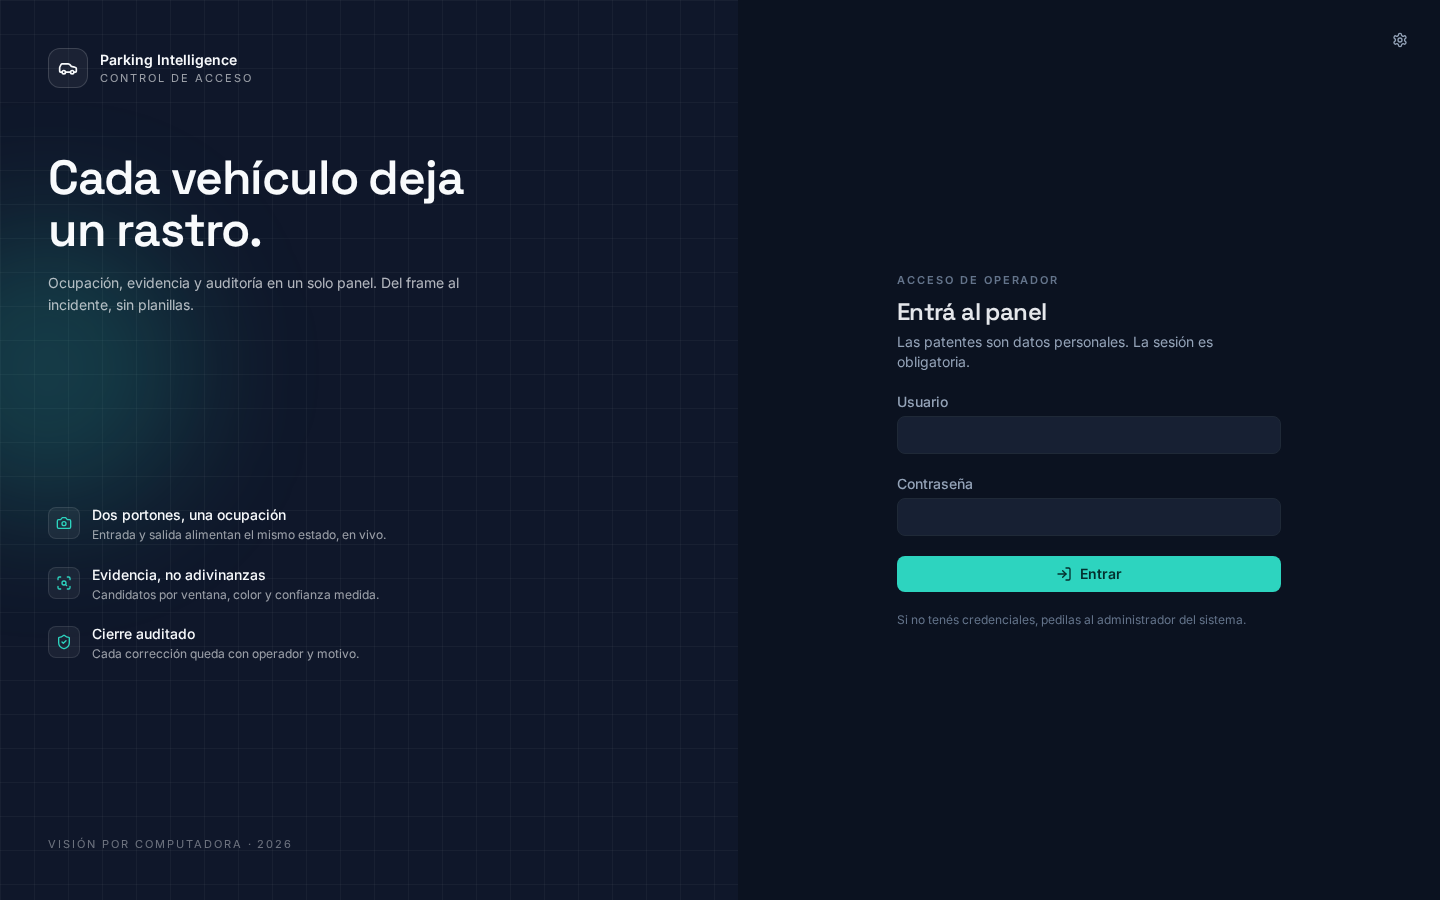
\includegraphics[width=0.92\textwidth]{fig_if_login.png}
    \caption{Pantalla de acceso a la aplicación.}
    \label{fig:if_login}
\end{figure}

\subsection{Panel de monitoreo}

El panel concentra el estado del recinto en una sola vista (Figura
\ref{fig:if_panel}). La columna izquierda presenta la ocupación como un medidor
con el número de vehículos dentro y la capacidad total; las tarjetas contiguas
resumen los ingresos del último día, la estadía promedio, la latencia del
percentil $95$ de la inferencia y la cantidad de cámaras que reportan latido.

Debajo se listan las cámaras con su puerta asignada y el instante de la última
señal, de modo que una cámara caída sea visible sin consultar registros. La lista
de vehículos activos expone, por cada sesión abierta, la matrícula, el tipo, el
color, la puerta de ingreso, el instante de entrada y el tiempo transcurrido,
junto con la acción de cierre manual. Las sesiones cuya permanencia excede el
umbral configurado se señalan con una marca de sesión huérfana: son las que
quedaron sin salida registrada y que el operador debe resolver. El panel de
eventos en vivo recibe las novedades por el canal persistente, y el gráfico
inferior presenta los ingresos de los últimos siete días.

\begin{figure}[htbp]
    \centering
    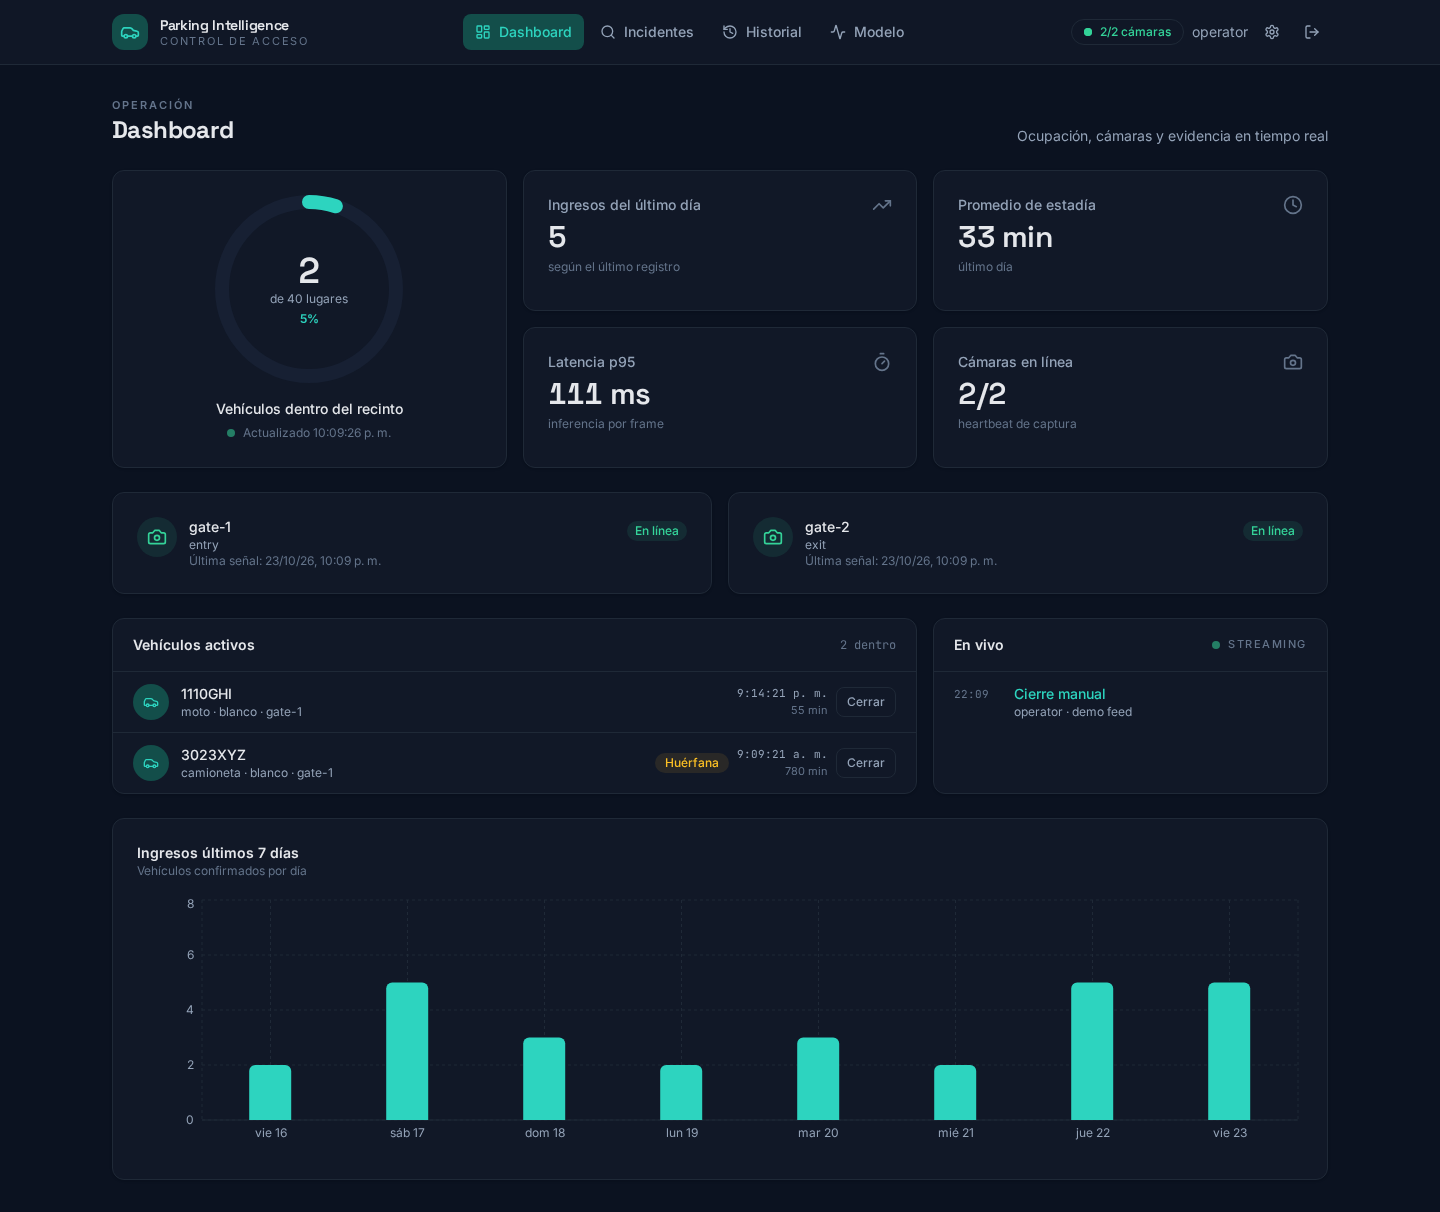
\includegraphics[width=0.95\textwidth]{fig_if_panel.png}
    \caption{Panel de monitoreo con la ocupación, el estado de las cámaras, las
    sesiones activas y el registro de eventos en vivo.}
    \label{fig:if_panel}
\end{figure}

Respecto del wireframe de la Figura~\ref{fig:wire_monitoreo}, la diferencia
principal es la ausencia del flujo de video. La decisión responde a un criterio de
costo y de arquitectura: transmitir video al navegador exige un servidor de
medios y ancho de banda continuo, mientras que el evento confirmado con su
recorte entrega la evidencia necesaria para auditar la decisión sin ese costo. La
contrapartida se asume: el operador no ve el movimiento en tiempo real, sino el
resultado de cada cruce.

\subsection{Búsqueda de incidentes y detalle del vehículo}

La vista de incidentes (Figura~\ref{fig:if_incidentes}) responde a la consulta
que motiva el sistema en la operación: qué vehículos pasaron por el acceso en una
ventana horaria determinada. El operador fija un intervalo ---por omisión, la hora
anterior y la siguiente al instante recordado--- y puede restringir por color. El
filtro de color es deliberadamente blando: incluye los vehículos cuya clasificación
está próxima al color pedido, porque el clasificador confunde tonos acromáticos y
un filtro estricto ocultaría el candidato buscado.

El resultado se presenta como una grilla de candidatos ordenada por cercanía al
instante consultado. Cada tarjeta muestra el recorte del vehículo, la matrícula
reconocida o la indicación de que no pudo leerse, el tipo y el color con su
confianza, y el instante de la observación. Los casos sin matrícula se conservan
en la lista: son precisamente los que el operador necesita revisar con la imagen.
Seleccionar una tarjeta abre el detalle del vehículo (Figura~\ref{fig:if_vehiculo}),
con el recorte de mayor tamaño disponible, los atributos con su confianza, el
identificador interno y la tabla de sesiones con ingreso, salida, duración, estado
y responsable del cierre.

\begin{figure}[htbp]
    \centering
    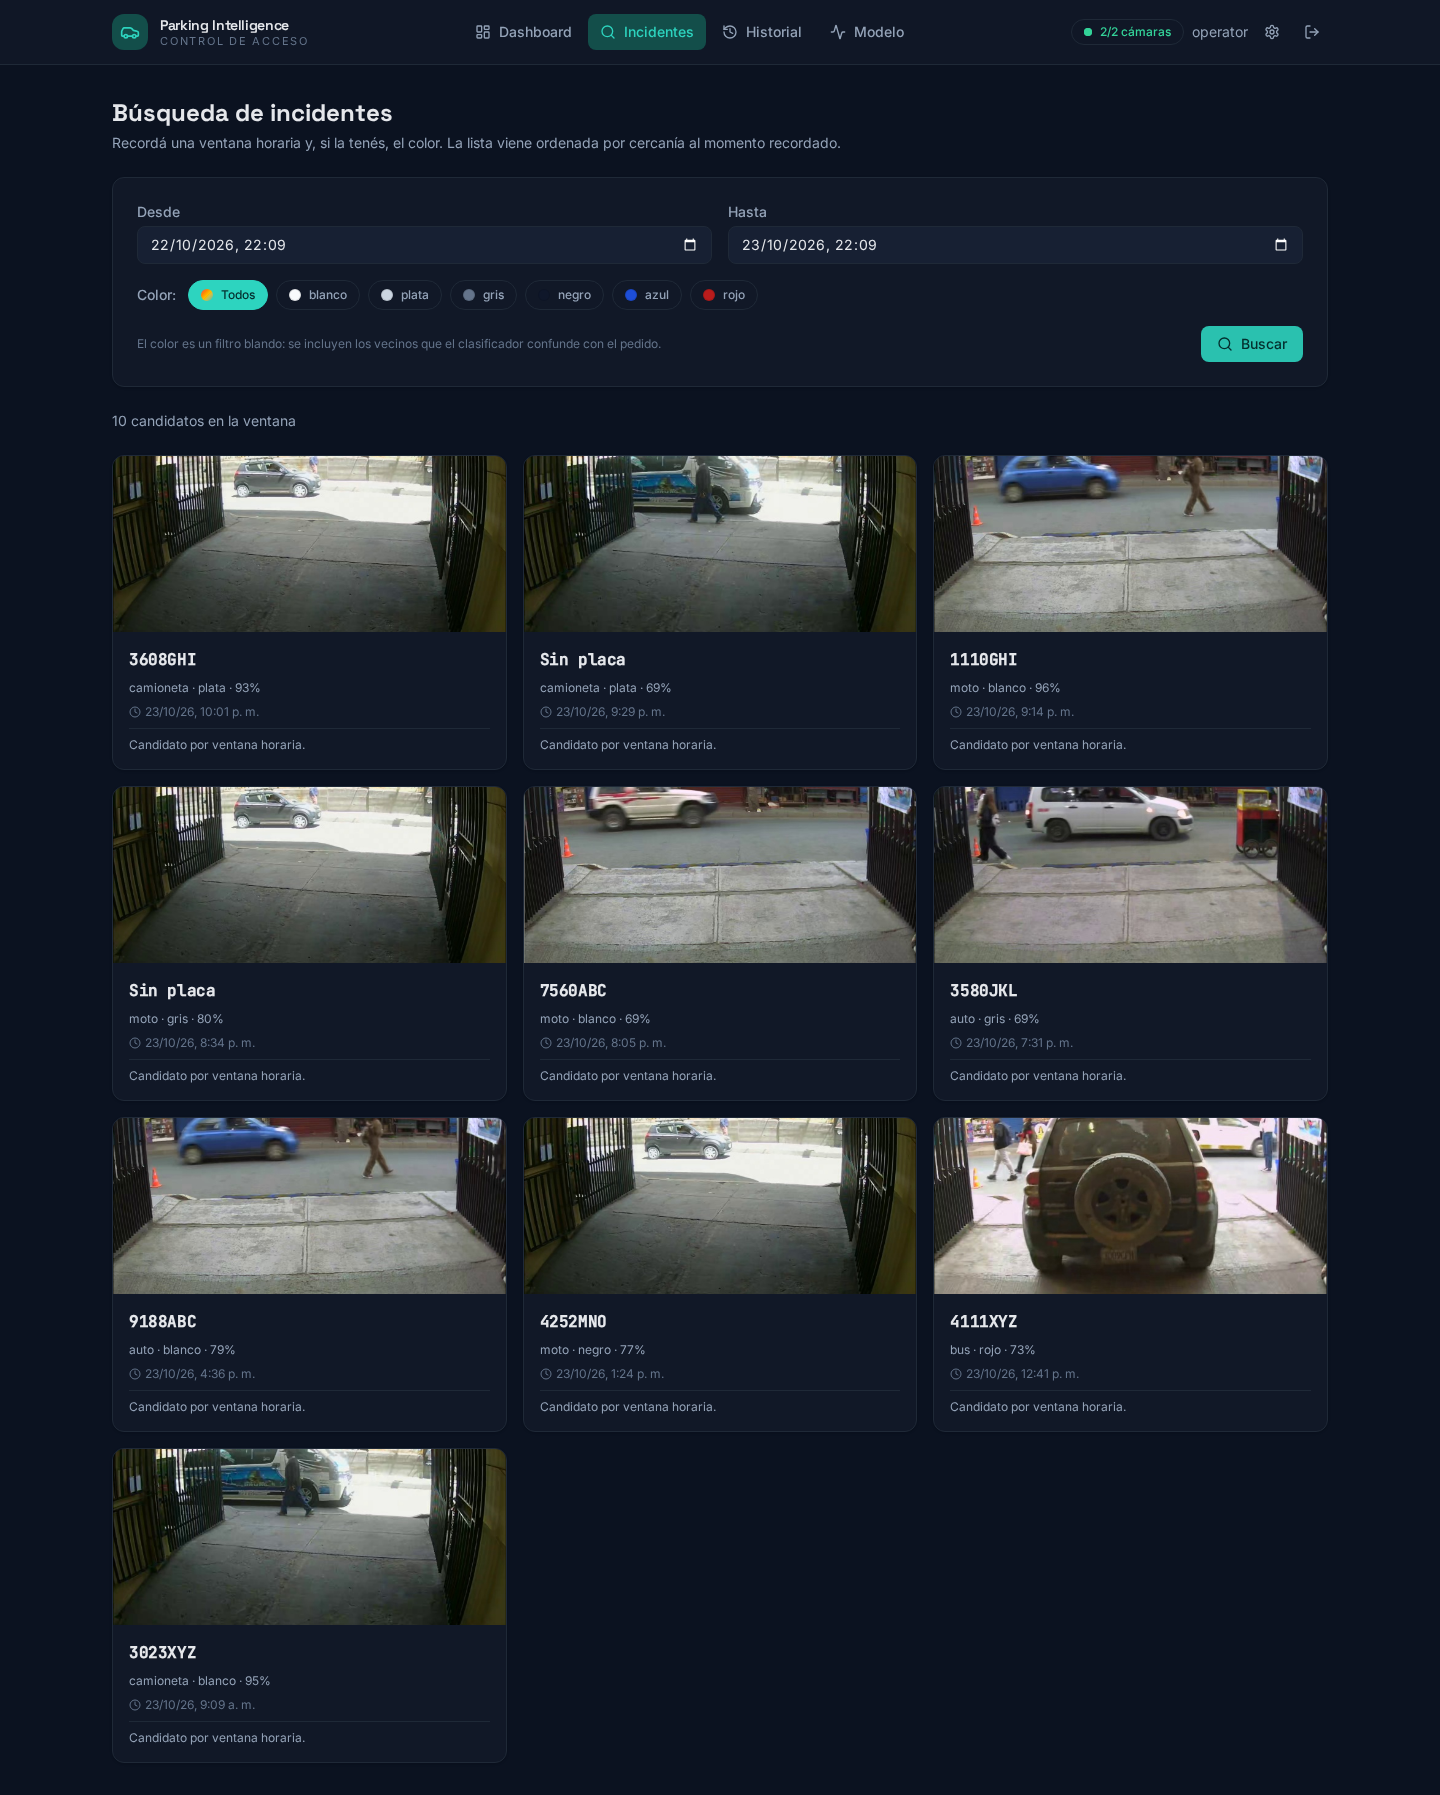
\includegraphics[width=0.95\textwidth]{fig_if_incidentes.png}
    \caption{Búsqueda de incidentes por ventana temporal y color, con los
    candidatos y su evidencia visual.}
    \label{fig:if_incidentes}
\end{figure}

\begin{figure}[htbp]
    \centering
    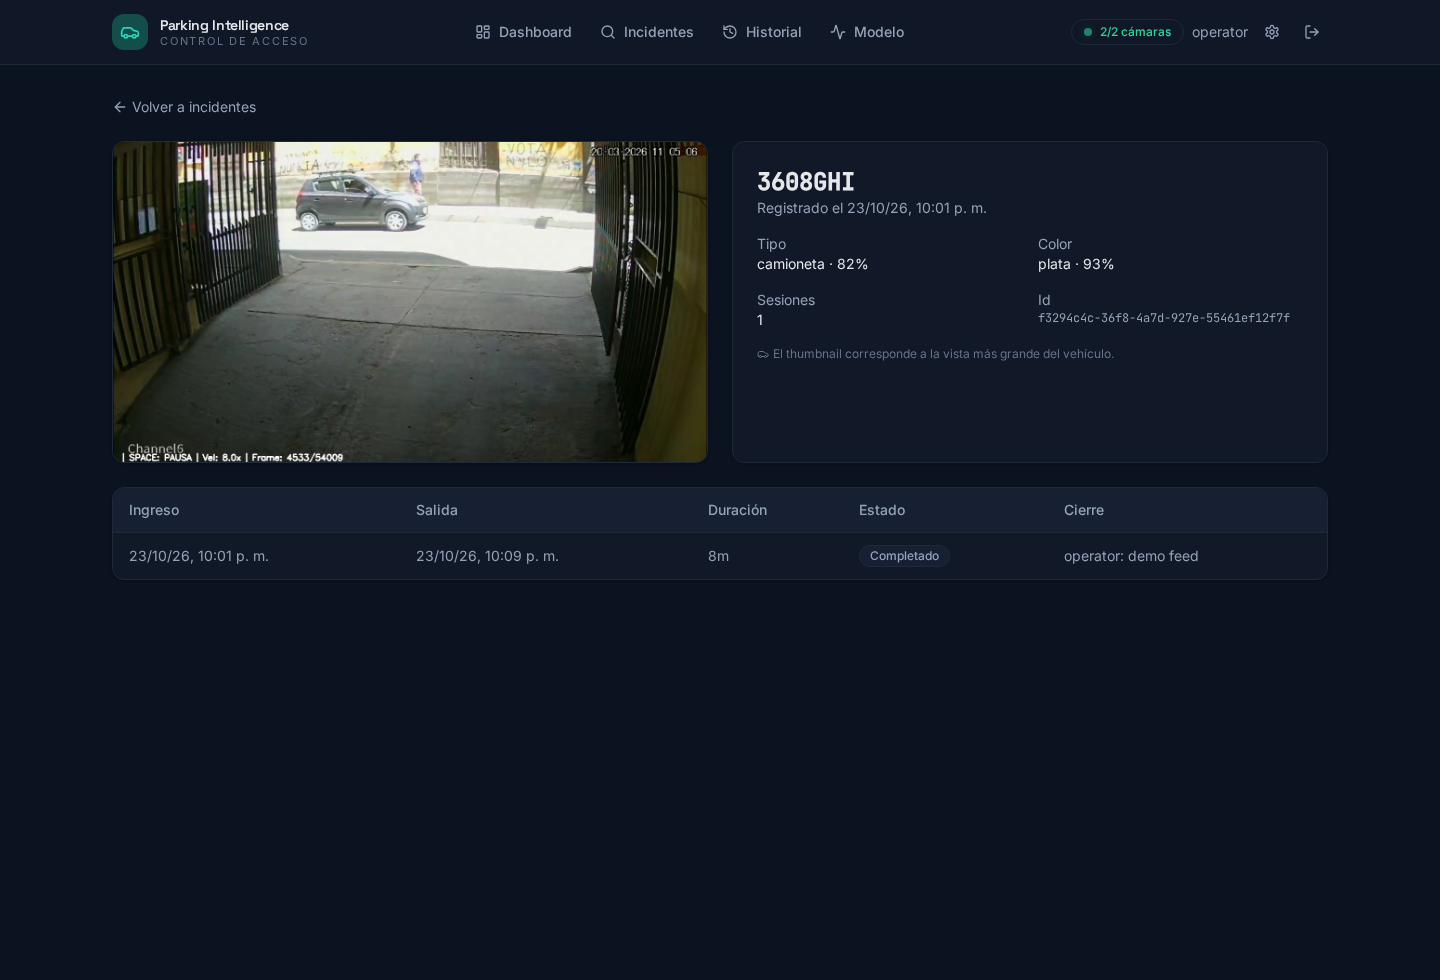
\includegraphics[width=0.95\textwidth]{fig_if_vehiculo.png}
    \caption{Detalle de un vehículo con su recorte, sus atributos y el historial
    de sesiones.}
    \label{fig:if_vehiculo}
\end{figure}

En el recorte del detalle se observa la información que el grabador superpone a la
imagen ---identificador de canal, marca temporal y contador de fotogramas---. Esa
superposición es la que el sistema anula antes de invocar al reconocimiento de
texto (Sección~\ref{subsec:ocr_crnn}): sin el enmascarado, el motor intentaría leer
caracteres que no pertenecen a la matrícula y produciría lecturas espurias.

\subsection{Historial de sesiones}

La vista de historial presenta una tabla con las sesiones registradas, ordenada de
la más reciente a la más antigua y con búsqueda por matrícula, tipo o color. Cada
fila expone la matrícula, el tipo, el color, el ingreso, la salida, la duración, el
estado de la sesión y el responsable del cierre. La consulta subyacente está
paginada por límite y desplazamiento, con un máximo de quinientos registros por
solicitud, y la vista solicita las doscientas más recientes. Su contenido es
tabular y coincide en columnas con el bloque inferior de la Figura
\ref{fig:if_vehiculo}, por lo que no se reproduce como figura independiente.

\subsection{Telemetría del modelo}

La vista de desempeño (Figura~\ref{fig:if_modelo}) no estaba prevista en el
diseño y se incorporó porque el sistema registra la latencia y la confianza de
cada evento confirmado. Presenta el total de eventos de la ventana, los modelos
que reportaron, el peor percentil $95$ de latencia y una tabla por modelo con la
confianza media y los percentiles $50$ y $95$ de la inferencia.

Su utilidad es diagnóstica: permite detectar una degradación de latencia o de
confianza sin recurrir a la base de datos. Conviene precisar su alcance para no
confundirla con una medición experimental: se alimenta de la telemetría de la
operación y está sujeta a la política de retención del sistema, de modo que
describe el comportamiento observado y no sustituye el banco comparativo por
formato de modelo que se declara pendiente en la Sección~\ref{sec:estado_gestion}.

\begin{figure}[htbp]
    \centering
    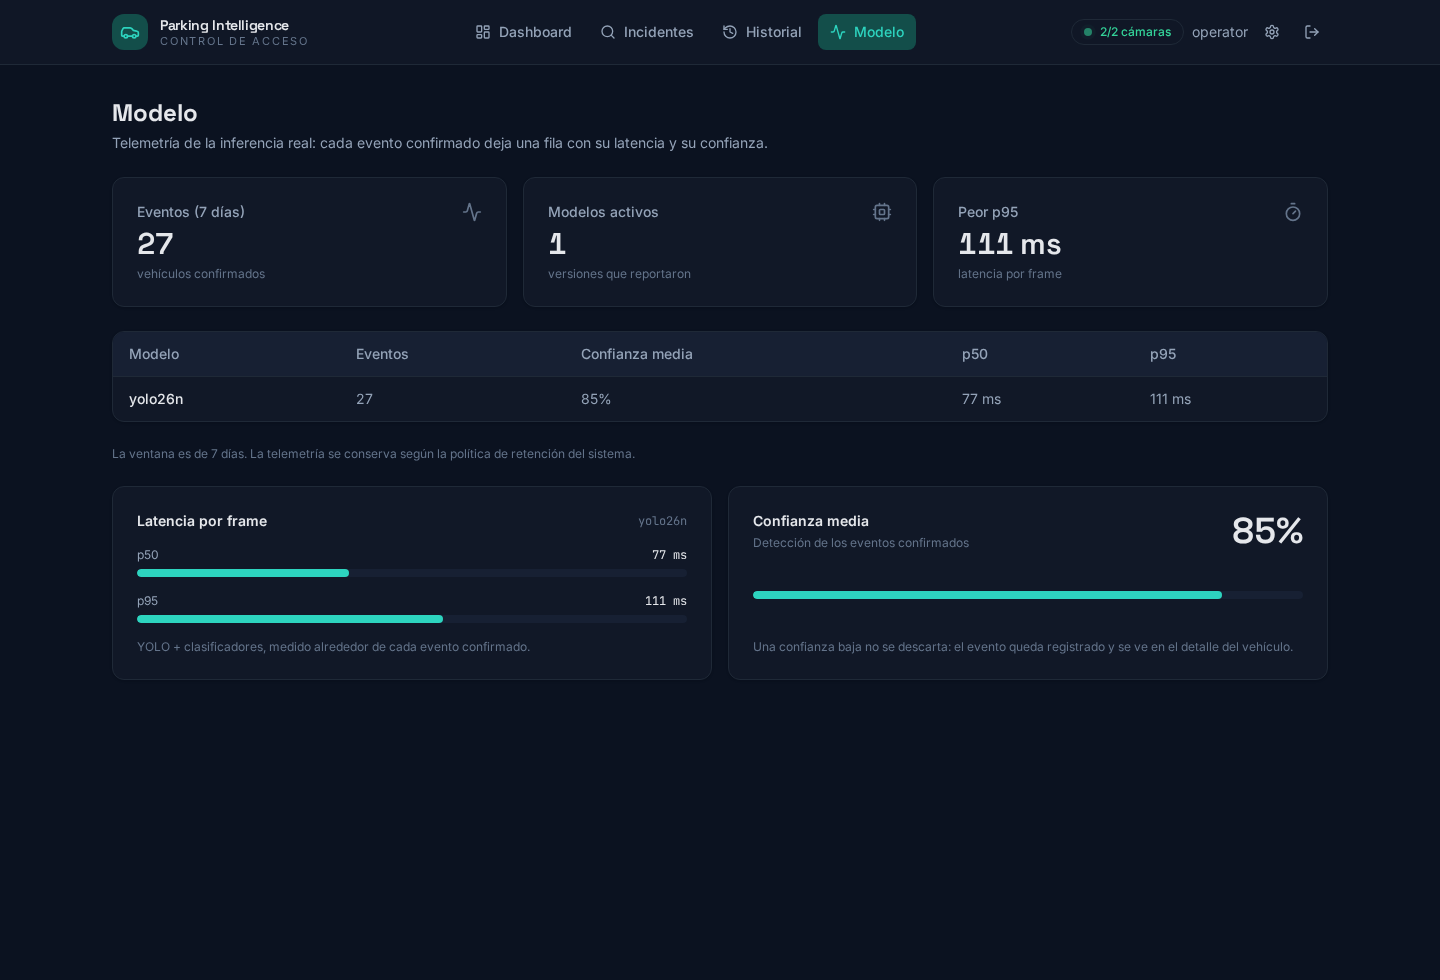
\includegraphics[width=0.95\textwidth]{fig_if_modelo.png}
    \caption{Telemetría del modelo: eventos, confianza media y latencia por
    percentil.}
    \label{fig:if_modelo}
\end{figure}

\subsection{Documentación de la interfaz de programación}

La especificación de la interfaz se genera de forma automática a partir de las
declaraciones de tipos de la aplicación y se publica en los formatos estándar de
OpenAPI. El documento resultante describe diecisiete rutas y trece esquemas de
datos, e incluye para cada operación sus parámetros, su cuerpo de solicitud, sus
respuestas y los códigos de error previstos. Al derivarse del mismo código que se
ejecuta, no puede desincronizarse de la implementación: un cambio en la firma de
un recurso se refleja en la especificación en el siguiente arranque.

La especificación no se reproduce como figura porque su valor probatorio está en
el documento generado y no en su representación visual. La Tabla
\ref{tab:api_implementada} enumera las rutas, y el documento completo se obtiene
desde el propio servicio, junto con una interfaz de exploración que permite
ejecutar cada operación contra el sistema en funcionamiento.


\chapter{Estimación de Costos}

\section{Introducción}

El presente capítulo estima el costo de desarrollo e implementación del sistema,
con el propósito de valorar económicamente el esfuerzo invertido y de determinar
la inversión requerida para su puesta en operación. La estimación se realiza
sobre artefactos verificables ---el software efectivamente construido y el
equipamiento efectivamente empleado--- y no sobre proyecciones abstractas.

El costo se descompone en dos partidas. La primera corresponde al
\textbf{desarrollo de software}, valorado a partir del tamaño funcional del
sistema según el método de puntos de función, contrastado con el tamaño del
código fuente medido directamente. La segunda corresponde al
\textbf{equipamiento} necesario para la operación, considerando que el proyecto
reutiliza la infraestructura de captura existente en el recinto y que, por
consiguiente, la inversión se concentra en la capacidad de cómputo.

Quedan explícitamente fuera del alcance de esta estimación los costos de
operación y mantenimiento posteriores a la puesta en marcha ---consumo
eléctrico, conectividad, soporte y conservación de los equipos---, así como el
costo de la infraestructura de captura preexistente, que no representa un
desembolso atribuible al proyecto.

Todas las valoraciones monetarias de este capítulo se expresan en bolivianos y
se declaran como parámetros de valoración ajustables, dado que dependen de
condiciones de mercado locales que exceden el alcance técnico del proyecto. La
metodología empleada permite recalcular la estimación ante una variación de
dichos parámetros sin alterar el análisis.

\section{Estimación del Costo de Software}

La valoración del software construido se apoya en el \textbf{análisis de puntos
de función} \cite{albrecht1979measuring,ifpug2010counting}, método estandarizado que mide el tamaño de un sistema a partir de las
funciones que ofrece al usuario y no de su implementación. Esta propiedad es la
que lo hace adecuado para el presente caso: permite valorar el sistema a partir
de los requerimientos y de la arquitectura documentados en los capítulos
precedentes, con independencia del lenguaje empleado y del estilo de codificación
del desarrollador.

Se descarta explícitamente el uso de modelos paramétricos de estimación
\cite{boehm1981software}
construidos para proyectos industriales. Esos modelos se calibran sobre equipos de
desarrollo, ciclos de vida prolongados y procesos organizacionales formalizados,
condiciones que no se verifican en un proyecto de grado de desarrollo individual.
Aplicarlos produciría una sobreestimación sin sustento; en su lugar se emplea un
método de medición funcional cuyo resultado es verificable.

\subsection{Tamaño funcional del sistema}

El recuento clasifica cada función en una de cinco categorías ---archivos lógicos
internos, archivos de interfaz externa, entradas externas, salidas externas y
consultas externas--- y le asigna una complejidad según la cantidad de tipos de
registro y de elementos de dato que manipula. La Tabla \ref{tab:puntos_funcion}
presenta el recuento resultante.

\begin{longtable}{
        P{0.10}
        P{0.55}
        P{0.16}
        P{0.09}
    }
    \caption{Recuento de puntos de función sin ajustar}
    \label{tab:puntos_funcion}\\

    \toprule
    \rowcolor{gray!20}
    \textbf{Tipo} &
    \textbf{Función} &
    \textbf{Complejidad} &
    \textbf{Puntos} \\
    \midrule
    \endfirsthead

    \multicolumn{4}{c}{\textit{Continuación de la Tabla
    \ref{tab:puntos_funcion}}} \\
    \toprule
    \rowcolor{gray!20}
    \textbf{Tipo} &
    \textbf{Función} &
    \textbf{Complejidad} &
    \textbf{Puntos} \\
    \midrule
    \endhead

    Archivo lógico & Vehículos observados: atributos identificados y matrícula & Baja & 7 \\
    \midrule
    Archivo lógico & Sesiones de estacionamiento: ingreso, salida y permanencia & Media & 10 \\
    \midrule
    Archivo lógico & Detecciones: bitácora de inferencia & Media & 10 \\
    \midrule
    Entrada externa & Registro de ingreso en el punto de acceso & Media & 4 \\
    \midrule
    Entrada externa & Registro de salida en el punto de acceso & Baja & 3 \\
    \midrule
    Entrada externa & Procesamiento del video archivado por el extractor & Media & 4 \\
    \midrule
    Salida externa & Agregados diarios de ocupación y permanencia & Media & 5 \\
    \midrule
    Salida externa & Notificación de variaciones de ocupación & Baja & 4 \\
    \midrule
    Salida externa & Generación del conjunto de datos anotado & Media & 5 \\
    \midrule
    Consulta externa & Sesiones actualmente activas & Baja & 3 \\
    \midrule
    Consulta externa & Historial de sesiones con paginación & Media & 4 \\
    \midrule
    Consulta externa & Nivel de ocupación del recinto & Baja & 3 \\
    \midrule
    \multicolumn{3}{r}{\textbf{Total sin ajustar}} & \textbf{62} \\*
    \multicolumn{4}{r}{\footnotesize\textit{Fuente: Elaboración propia}} \\*
    \bottomrule
\end{longtable}

La complejidad se asignó según el número de tipos de registro y de elementos de
dato que cada función manipula. Se clasificaron como de complejidad baja las
funciones que operan sobre una única estructura de datos con un número reducido
de campos, y como de complejidad media aquellas que involucran una relación entre
dos entidades o que devuelven información derivada de un cálculo agregado. No se
clasificó ninguna función como de complejidad alta, dado que la estructura de
datos del sistema es acotada y no contiene relaciones de tercer nivel ni
agrupaciones jerárquicas complejas.

Al recuento sin ajustar se aplica el factor de ajuste que pondera catorce
características generales del sistema. Su valor se adopta como la unidad por las
siguientes razones: las características que incrementarían el factor ---exigencia
de desempeño, procesamiento complejo derivado del tratamiento de imágenes, y
facilidad de operación e instalación--- se compensan con aquellas que lo
reducirían ---ausencia de procesamiento distribuido, de operación en múltiples
sitios y de necesidad de integración con sistemas externos---. El tamaño funcional
ajustado resulta, en consecuencia, de \textbf{62 puntos de función}.

\subsection{Contraste con el tamaño medido del código}

Una verificación independiente del recuento anterior se obtiene midiendo el
código fuente efectivamente escrito. La Tabla \ref{tab:lineas_codigo} presenta el
resultado del conteo por área.

\begin{longtable}{
        P{0.64}
        P{0.14}
        P{0.14}
    }
    \caption{Tamaño del código fuente por área}
    \label{tab:lineas_codigo}\\

    \toprule
    \rowcolor{gray!20}
    \textbf{Área} &
    \textbf{Archivos} &
    \textbf{Líneas} \\
    \midrule
    \endfirsthead

    \multicolumn{3}{c}{\textit{Continuación de la Tabla
    \ref{tab:lineas_codigo}}} \\
    \toprule
    \rowcolor{gray!20}
    \textbf{Área} &
    \textbf{Archivos} &
    \textbf{Líneas} \\
    \midrule
    \endhead

    Dominio (reglas de negocio y puertos) & 10 & 615 \\
    \midrule
    Aplicación (casos de uso) & 2 & 182 \\
    \midrule
    Adaptadores (base de datos, cola, bus y modelos) & 18 & 1,234 \\
    \midrule
    Entrada HTTP (rutas, esquemas y configuración) & 18 & 1,408 \\
    \midrule
    Trabajador de inferencia & 5 & 349 \\
    \midrule
    Migraciones del esquema & 4 & 236 \\
    \midrule
    Captura de flujos de video & 2 & 361 \\
    \midrule
    Cliente web & 29 & 2,561 \\
    \midrule
    \textbf{Subtotal del producto} & \textbf{88} & \textbf{6,946} \\
    \midrule
    Pruebas del servicio y de las herramientas & 40 & 3,537 \\
    \midrule
    Herramientas de datos y entrenamiento & 31 & 6,225 \\
    \midrule
    \textbf{Total entregado} & \textbf{159} & \textbf{16,708} \\*
    \multicolumn{3}{r}{\footnotesize\textit{Fuente: Elaboración propia}} \\*
    \bottomrule
\end{longtable}

El código se mide sobre los archivos fuente efectivamente entregados, excluyendo
las dependencias de terceros, los artefactos generados y los archivos de
inicialización de paquete, que no contienen lógica. El conteo distingue dos
naturalezas: el \textbf{producto}, que implementa las funciones del sistema, y el
material de \textbf{verificación y de construcción de datos}, que sostiene el
trabajo pero no forma parte de la interfaz ofrecida al usuario.

Ambas mediciones son independientes entre sí: el tamaño funcional se derivó de
las funciones documentadas y el tamaño del código, de los archivos fuente. La
relación obtenida sobre el producto ---$6{,}946$ líneas para $62$ puntos de
función, es decir aproximadamente $112$ líneas por punto de función--- constituye
una verificación de consistencia interna del análisis. Las pruebas y las
herramientas de datos se informan por transparencia, pero se excluyen de esa
relación: contarlas elevaría el cociente a cerca de $270$ líneas por punto de
función y describiría el esfuerzo de construcción del conjunto de datos, no el
tamaño funcional del sistema entregado.

\subsection{Esfuerzo y costo de desarrollo}

El esfuerzo de desarrollo se obtiene a partir del tamaño funcional y de una
productividad de referencia, y el costo, a partir del esfuerzo y de una tarifa:

\begin{equation}
    E = TFA \cdot P \qquad\qquad C_{\text{software}} = E \cdot T
\end{equation}

donde $TFA$ es el tamaño funcional ajustado ---$62$ puntos de función---, $P$ la
productividad expresada en horas por punto de función, $E$ el esfuerzo en horas,
$C_{\text{software}}$ el costo de desarrollo y $T$ la tarifa horaria.

Los dos parámetros de valoración ---productividad y tarifa--- dependen de
condiciones locales de mercado y de la experiencia del desarrollador, y no son
derivables del análisis técnico. Se declaran de forma explícita en la Tabla
\ref{tab:parametros_costo} para que la estimación pueda reproducirse y
recalcularse.

\begin{longtable}{
        P{0.30}
        P{0.12}
        P{0.12}
        P{0.36}
    }
    \caption{Parámetros de valoración del costo de software}
    \label{tab:parametros_costo}\\

    \toprule
    \rowcolor{gray!20}
    \textbf{Parámetro} &
    \textbf{Símbolo} &
    \textbf{Valor} &
    \textbf{Procedencia} \\
    \midrule
    \endfirsthead

    \multicolumn{4}{c}{\textit{Continuación de la Tabla
    \ref{tab:parametros_costo}}} \\
    \toprule
    \rowcolor{gray!20}
    \textbf{Parámetro} &
    \textbf{Símbolo} &
    \textbf{Valor} &
    \textbf{Procedencia} \\
    \midrule
    \endhead

    Tamaño funcional ajustado & $TFA$ & 62 puntos & Calculado en el apartado anterior. \\
    \midrule
    Productividad & $P$ & $12$ horas por punto & Parámetro declarado. \\
    \midrule
    Esfuerzo & $E$ & $744$ horas & $TFA \cdot P$. \\
    \midrule
    Tarifa horaria & $T$ & Bs $30$ & Parámetro declarado. \\
    \midrule
    Costo de desarrollo & $C_{\text{software}}$ & Bs 22,320 & $E \cdot T$. \\*
    \multicolumn{4}{r}{\footnotesize\textit{Fuente: Elaboración propia}} \\*
    \bottomrule
\end{longtable}

Los valores adoptados se declaran de la siguiente forma. La productividad se fija
en $12$ horas por punto de función, equivalentes a $744$ horas de dedicación para
el tamaño calculado; el valor se adopta por analogía con proyectos de magnitud
comparable desarrollados en lenguajes de alto nivel, y es coherente con un
desarrollo individual de varios meses. La tarifa se fija en Bs $30$ por hora, que
corresponde a un salario mensual de referencia de Bs 4,800 sobre una jornada de
$160$ horas. Con ambos parámetros, el costo de desarrollo resulta de Bs 22,320.

La estimación es sensible a la tarifa y no al tamaño: con una tarifa de Bs $20$
el costo de software desciende a Bs 14,880, y con Bs $40$ asciende a Bs 29,760,
mientras que el tamaño funcional permanece fijo porque se deriva de las
funciones documentadas y no del esfuerzo invertido. Los dos parámetros son de
mercado y deben reemplazarse por la cotización vigente al momento de la
presentación; la estructura del cálculo no cambia al hacerlo.

\section{Estimación del Equipamiento}

La estimación del equipamiento parte de una condición favorable del proyecto: la
infraestructura de captura ya existe en el recinto y se reutiliza. El sistema no
requiere la instalación de cámaras nuevas, sino que consume el flujo de video
producido por el grabador digital que opera el parqueadero. En consecuencia, la
inversión se concentra en la capacidad de cómputo necesaria para ejecutar la
inferencia y en el almacenamiento requerido para el material de video y los
conjuntos de datos derivados.

La Tabla \ref{tab:equipamiento} enumera los elementos considerados. Se distingue
entre los elementos que representan un desembolso atribuible al proyecto y
aquellos que se reutilizan de la infraestructura existente y que, por tanto, no
se computan como inversión.

\begin{longtable}{
        P{0.25}
        P{0.35}
        P{0.12}
        P{0.18}
    }
    \caption{Equipamiento requerido por el proyecto}
    \label{tab:equipamiento}\\

    \toprule
    \rowcolor{gray!20}
    \textbf{Elemento} &
    \textbf{Especificación} &
    \textbf{Cantidad} &
    \textbf{Costo} \\
    \midrule
    \endfirsthead

    \multicolumn{4}{c}{\textit{Continuación de la Tabla
    \ref{tab:equipamiento}}} \\
    \toprule
    \rowcolor{gray!20}
    \textbf{Elemento} &
    \textbf{Especificación} &
    \textbf{Cantidad} &
    \textbf{Costo} \\
    \midrule
    \endhead

    Equipo de cómputo con acelerador gráfico &
    GPU NVIDIA GeForce RTX 3050 (4 GB de memoria), procesador de 12 núcleos,
    15 GiB de memoria principal &
    1 & Bs 10.000 \\
    \midrule

    Almacenamiento externo &
    Unidad de $1{,}9$ TB destinada al material de video y a los conjuntos de datos &
    1 & Bs 850 \\
    \midrule

    Infraestructura de captura &
    Grabador digital y cámaras de los puntos de acceso, preexistentes en el
    recinto &
    --- & Sin desembolso \\
    \midrule

    Red y energía &
    Infraestructura de red local y suministro eléctrico del recinto &
    --- & Sin desembolso \\
    \midrule

    Licencias de software &
    Totalidad del componente de software bajo licencias de código abierto &
    --- & Sin desembolso \\
    \midrule

    \multicolumn{3}{r}{\textbf{Total de equipamiento}} & \textbf{Bs 10.850} \\*
    \multicolumn{4}{r}{\footnotesize\textit{Fuente: Elaboración propia}} \\*
    \bottomrule
\end{longtable}

El dimensionamiento del almacenamiento se deriva del volumen efectivo del
material procesado. La captura del recinto se realiza a una resolución de
$1280 \times 720$ píxeles, a una tasa de quince fotogramas por segundo y con
codificación de alta eficiencia, lo que produce aproximadamente 6,7 GB por cada
treinta horas de registro. La generación de los conjuntos de datos añade, a su
vez, poco más de 3 GB derivados del mismo material. Estas cifras sitúan los
requerimientos de almacenamiento muy por debajo de la capacidad disponible, pero
justifican su consideración explícita: el proceso de extracción recorre
repetidamente el archivo de video y requiere conservar simultáneamente las
muestras emitidas.

El equipo de cómputo merece una precisión. El acelerador gráfico empleado dispone
de apenas 4 GB de memoria, un orden de magnitud inferior al de los equipos
habitualmente asociados al entrenamiento de modelos de detección. Esta
restricción no es un inconveniente del proyecto sino su condición de contorno:
constituye la evidencia de que el sistema puede operar sobre hardware de gama
moderada, que es precisamente el escenario de despliegue para el que se diseñó la
estrategia de optimización descrita en el capítulo anterior. El mismo equipo
ejecuta el servicio de gestión, el trabajador de inferencia y la base de datos
como contenedores, sin requerir un servidor dedicado, lo que elimina una partida
de inversión que el diseño evita por construcción.

Respecto de las licencias, la totalidad de los componentes empleados ---lenguaje,
marco de trabajo web, motor de base de datos, cola de tareas, bibliotecas de
aprendizaje profundo, motor de reconocimiento de texto y biblioteca de interfaz---
se distribuye bajo licencias de código abierto, de modo que no generan costo de
adquisición. Se deja constancia, no obstante, de que la biblioteca de detección
empleada se distribuye bajo una licencia con obligaciones de reciprocidad que
condicionan su uso en un producto comercial cerrado; esta consideración no afecta
al presente proyecto, de carácter académico, pero resulta relevante para una
eventual explotación comercial del sistema.

Los precios unitarios se declaran a la fecha de cierre del documento: Bs 10.000
para el equipo de cómputo y Bs 850 para la unidad de almacenamiento, lo que
arroja un total de Bs 10.850. Al igual que la tarifa horaria, son parámetros de
mercado sujetos a variación y deben reemplazarse por cotización formal antes de la
presentación. La partida es pequeña frente al costo de desarrollo, de modo que una
variación de precios en el equipamiento no altera la conclusión del análisis
económico.

\section{Costo Total Estimado}

El costo total del proyecto resulta de la suma de las dos partidas estimadas:

\begin{equation}
    C_{\text{total}} = C_{\text{software}} + C_{\text{equipamiento}}
\end{equation}

La Tabla \ref{tab:costo_total} presenta la estructura de la estimación.

\begin{longtable}{
        P{0.25}
        P{0.52}
        P{0.15}
    }
    \caption{Estructura del costo total estimado}
    \label{tab:costo_total}\\

    \toprule
    \rowcolor{gray!20}
    \textbf{Partida} &
    \textbf{Composición} &
    \textbf{Valor} \\
    \midrule
    \endfirsthead

    \multicolumn{3}{c}{\textit{Continuación de la Tabla
    \ref{tab:costo_total}}} \\
    \toprule
    \rowcolor{gray!20}
    \textbf{Partida} &
    \textbf{Composición} &
    \textbf{Valor} \\
    \midrule
    \endhead

    Costo de software &
    $62$ puntos de función $\times$ $12$ horas por punto $\times$ Bs $30$ por hora &
    Bs 22,320 \\
    \midrule

    Costo de equipamiento &
    Equipo de cómputo con acelerador gráfico y almacenamiento externo &
    Bs 10,850 \\
    \midrule

    \multicolumn{2}{r}{\textbf{Costo total del proyecto}} & \textbf{Bs 33,170} \\*
    \multicolumn{3}{r}{\footnotesize\textit{Fuente: Elaboración propia}} \\*
    \bottomrule
\end{longtable}

Dos observaciones corresponden a esta estructura. La primera es que la partida de
software domina la estimación ---cerca del $67\%$ del total--- porque el proyecto
no requiere adquirir infraestructura de captura ni licencias, de manera que el
valor del desarrollo concentra la mayor parte del costo. La segunda es que la
estimación se sostiene sobre \textbf{parámetros declarados} ---productividad,
tarifa horaria y precios de equipo--- y no sobre supuestos implícitos, lo que
permite recalcularla ante una variación de las condiciones de mercado sin
modificar el análisis técnico.

La valoración monetaria queda así cerrada con los parámetros declarados: Bs
33,170 como costo total, de los cuales Bs 22,320 corresponden al desarrollo y
Bs 10,850 al equipamiento. Desde el punto de vista metodológico, la estimación
establece un tamaño funcional verificable ---$62$ puntos de función--- corroborado
por una medición independiente del código ---$6{,}946$ líneas de producto en $88$
archivos---, que constituye la base trazable de cualquier valoración posterior.


\chapter{Conclusiones y Recomendaciones}

\section{Introducción}

El presente capítulo cierra el trabajo contrastando lo construido con lo
comprometido. No se limita a resumir los capítulos precedentes: recorre uno por
uno los objetivos específicos y las hipótesis declarados en el perfil, y para
cada uno establece si la evidencia lo respalda, lo refuta o no alcanza a
pronunciarse. Esa distinción es el aporte central de este capítulo, porque un
sistema complejo rara vez se comporta de forma uniforme: algunos componentes
superan el umbral exigido, otros quedan por debajo y otros no llegaron a
medirse.

El capítulo se organiza en tres partes. La primera sintetiza el sistema
efectivamente construido y delimita qué puede afirmarse de él. La segunda
contrasta la hipótesis general y cada hipótesis específica, y dedica un apartado
propio a la brecha del reconocimiento de matrículas, por ser el componente donde
la distancia entre el criterio comprometido y el resultado medido es mayor. La
tercera formula las recomendaciones que se desprenden de esas mediciones,
distinguiendo las que corresponden a la continuidad inmediata del sistema de
aquellas que constituyen líneas de trabajo posteriores.

Se mantiene a lo largo del capítulo una regla de escritura: ningún resultado se
presenta sin la condición que lo produjo, y ninguna limitación se enuncia sin
indicar qué la causa y qué la removería. Un trabajo que declara sus brechas con
precisión es más útil que uno que las disimula, porque permite que el siguiente
investigador sepa exactamente dónde estaba el límite y por qué.

\section{Conclusiones}

\subsection{Síntesis del sistema construido}

El trabajo entrega un sistema de gestión de acceso vehicular ensamblado a partir
de dos subsistemas con responsabilidades separadas. El subsistema de visión
encadena detección de vehículos sobre pesos preentrenados, seguimiento
multiobjeto, un detector de placas entrenado para este dominio, un reconocedor de
matrículas con arquitectura ResNet18--BiLSTM--CTC y dos clasificadores de
atributos. El subsistema de gestión expone diecisiete rutas HTTP ---operativas, de consulta,
de autenticación y de diagnóstico--- y un canal persistente de notificación sobre
FastAPI, PostgreSQL y una cola de tareas, y ofrece un cliente web con seis vistas. El despliegue se resuelve con contenedores,
exportación a formatos intermedios y compilación de motores especializados para el
acelerador de destino.

La magnitud del artefacto es verificable y no estimada: el sistema comprende $62$
puntos de función y $6.946$ líneas de producto distribuidas en $88$ archivos, a
las que se suman $3.537$ líneas de pruebas y $6.225$ de herramientas de datos. El
conjunto de datos que lo sustenta también es verificable: $496$ matrículas reales
confirmadas por un operador, $359.992$ matrículas sintéticas con formato
boliviano, $4.006$ recortes de vehículo y $868$ recortes de placa con caja
revisada manualmente.

Esa verificabilidad alcanza al software. El subsistema de gestión se encuentra
integrado con el motor de visión: la tarea de inferencia decodifica el fotograma,
invoca al motor, agrega las detecciones por trayectoria y persiste el vehículo, la
sesión y la observación de forma atómica, con la latencia de inferencia registrada
por fotograma. El esquema se materializa en tres revisiones de migración que se
aplican en orden, el cierre de sesión opera por emparejamiento exacto de matrícula
con umbral de confianza y admite el cierre manual auditado, y la aplicación web
ofrece seis vistas. La verificación automática comprende $140$ pruebas unitarias y
$4$ de integración que se ejecutan contra una base PostgreSQL real con las
migraciones aplicadas, con una cobertura del $88\%$ sobre el código de la
aplicación.

El límite que corresponde declarar es de otra naturaleza. El contraste de la
matrícula contra un padrón de vehículos habilitados, previsto como requerimiento
RF-10, no forma parte de la entrega: la entidad de vehículos registra los
vehículos observados en los accesos, no un padrón previo. Lo que tampoco se
realizó es la \textbf{validación de campo de extremo a extremo}: la cadena
completa con las cámaras del recinto y la simulación con las dos fuentes
sincronizadas. Esa validación es la que sostendría la medición de la determinación
de eventos ($H_{1.5}$) y la que permitiría afirmar que el sistema opera como un
todo continuo, y no solo que cada componente funciona y está probado. En
consecuencia, los resultados que se reportan corresponden a los componentes
efectivamente ejecutados y se atribuyen a ellos, no a una operación en condiciones
reales de recinto.

\subsection{Contrastación de la hipótesis general}

La hipótesis general exige que el sistema alcance simultáneamente los criterios
de desempeño establecidos para la detección e identificación de vehículos, el
reconocimiento de placas y la determinación de eventos. Por su forma conjuntiva,
basta que un solo término no se cumpla para que la hipótesis no se respalde, y
basta que un término no se haya medido para que no pueda declararse verificada.

El estado de cada término se resume en la Tabla~\ref{tab:contraste_hipotesis}:
dos criterios se cumplen (identificación de tipo y detección de placas), tres no
se alcanzan (color predominante, exactitud por carácter y coincidencia exacta) y
dos no fueron medidos (detección de vehículos y determinación de eventos).

\textbf{La hipótesis general no se respalda.} Dos de sus componentes medidos
quedan por debajo del umbral comprometido, de modo que el sistema, en su estado
actual, no satisface el conjunto de criterios que la hipótesis exige. Se acepta
la hipótesis nula para esos componentes.

La conclusión debe formularse con una precisión adicional: la hipótesis nula
tampoco queda demostrada en su totalidad, porque dos de sus términos no fueron
sometidos a medición. Respecto de la detección de vehículos y de la determinación
de eventos, el trabajo no afirma que el sistema falle ni que acierte: afirma que
no lo sabe, y explicita por qué. Un pronunciamiento en cualquiera de las dos
direcciones carecería de respaldo experimental.

\subsection{Cumplimiento de los objetivos específicos}

La Tabla~\ref{tab:cumplimiento_objetivos} contrasta cada objetivo específico con
la evidencia producida y con el grado de cumplimiento que esa evidencia sostiene.
Se emplean tres estados: \emph{cumplido} cuando el objetivo se alcanzó y su
resultado es verificable; \emph{parcial} cuando el artefacto existe y fue
evaluado, pero algún criterio asociado no se alcanzó o alguna medición quedó
pendiente; y \emph{no cumplido} cuando no existe evidencia que lo respalde. En
este trabajo no se registra ningún objetivo en el tercer estado.

\begin{longtable}{
        P{0.30}
        P{0.12}
        P{0.50}
    }
    \caption{Cumplimiento de los objetivos específicos}
    \label{tab:cumplimiento_objetivos}\\

    \toprule
    \rowcolor{gray!20}
    \textbf{Objetivo específico} &
    \textbf{Estado} &
    \textbf{Evidencia y observación} \\
    \midrule
    \endfirsthead

    \multicolumn{3}{c}{\textit{Continuación de la Tabla
    \ref{tab:cumplimiento_objetivos}}} \\
    \toprule
    \rowcolor{gray!20}
    \textbf{Objetivo específico} &
    \textbf{Estado} &
    \textbf{Evidencia y observación} \\
    \midrule
    \endhead

    Analizar las condiciones de operación, los puntos de acceso y los
    requerimientos técnicos y funcionales. &
    Cumplido &
    Requerimientos funcionales, no funcionales y de infraestructura
    especificados con identificadores trazables; condiciones de captura,
    iluminación y ángulo caracterizadas a partir del material recolectado. \\
    \midrule

    Construir y preparar un conjunto de datos representativo de las condiciones
    reales. &
    Cumplido &
    $496$ matrículas reales verificadas por operador, $359.992$ sintéticas,
    $4.006$ recortes de vehículo y $868$ recortes de placa con caja revisada.
    Partición por sesión y por bloque horario, sin sesiones compartidas entre
    entrenamiento y prueba. El volumen real es la restricción dominante del
    módulo de reconocimiento y así se declara. \\
    \midrule

    Adaptar y entrenar modelos de detección e identificación de tipo y color, y
    de localización de placas. &
    Parcial &
    Tipo de vehículo: F1 macro $0{,}8887$ sobre el umbral de $0{,}85$. Color:
    F1 macro $0{,}8124$ bajo el umbral. Localización de placas: exhaustividad
    $0{,}9714$ y mAP@50 $0{,}9898$. Detección de vehículos: el modelo opera con
    pesos preentrenados sin ajuste fino y su mAP no fue medido por ausencia de
    cajas de referencia humana. \\
    \midrule

    Desarrollar y entrenar un modelo de reconocimiento óptico de caracteres para
    placas vehiculares y evaluarlo bajo distintas condiciones de visibilidad. &
    Parcial &
    Modelo construido y entrenado en dos etapas, evaluado sobre $101$ placas
    aisladas y sobre $88$ recortes de vehículo con texto verificado. Exactitud
    por carácter $0{,}789$ y $0{,}737$; coincidencia exacta $0{,}356$ y
    $0{,}261$. El criterio de $0{,}90$ de exactitud por carácter no se alcanza;
    la causa se analiza en la Subsección~\ref{subsec:brecha_ocr}. \\
    \midrule

    Integrar los modelos en un sistema de gestión con registro y consulta de
    eventos. &
    Cumplido &
    Modelo de datos con restricciones e índices, tres revisiones de migración,
    diecisiete rutas HTTP, canal persistente de notificación, cliente web con seis
    vistas y emparejamiento de salida con abstención.
    Verificado por $140$ pruebas unitarias y $4$ de integración contra una base
    real. La validación de extremo a extremo con las cámaras del recinto
    corresponde al objetivo de evaluación, no a este. \\
    \midrule

    Evaluar el desempeño del sistema y el efecto de las técnicas de
    optimización. &
    Parcial &
    Cinco de los siete términos de hipótesis fueron medidos sobre conjuntos de
    prueba independientes. La optimización fue aplicada y su efecto sobre la
    huella en disco está cuantificado (reducción del $75\%$ al pasar de precisión
    simple a media precisión), pero la latencia, la tasa de fotogramas y la
    degradación de exactitud atribuible a la cuantización no llegaron a medirse. \\
    \bottomrule
    \multicolumn{3}{r}{\footnotesize\textit{Fuente: Elaboración propia}} \\*
\end{longtable}

Los tres objetivos parciales comparten un mismo patrón: el artefacto se
construyó, se ejecutó y se midió, pero la medición no alcanzó el umbral
comprometido o no cubrió todos los términos previstos. Ninguno de los tres
constituye un objetivo abandonado. Se trata de objetivos cuyo cumplimiento está
acotado por condiciones que este apartado identifica y que las recomendaciones
traducen en trabajo concreto.

\subsection{La brecha del reconocimiento de matrículas}
\label{subsec:brecha_ocr}

Es el componente de mayor distancia entre lo comprometido y lo obtenido, y por
eso recibe un tratamiento propio. El criterio exigía, de forma simultánea,
exhaustividad de detección igual o superior al $90\%$ y exactitud por carácter
igual o superior al $90\%$, con una coincidencia exacta adicional del $80\%$. El
componente de detección se cumplió con holgura ($0{,}9714$ de exhaustividad y
$0{,}9898$ de mAP@50). El déficit es íntegramente de reconocimiento: $0{,}789$ de
exactitud por carácter sobre recortes aislados y $0{,}737$ sobre el sistema
ensamblado, con coincidencia exacta de $0{,}356$ y $0{,}261$ respectivamente.

La conclusión que sostiene la evidencia es que \textbf{la restricción dominante
no es la arquitectura del modelo, sino la calidad y el volumen del material
disponible}. Cuatro mediciones independientes convergen en esa dirección.

\paragraph{Primera causa: la resolución física del recorte.}
Un recorte de $40 \times 13$ píxeles que contiene siete caracteres dispone de
aproximadamente cinco píxeles de ancho por glifo. A esa escala la información no
está presente en la imagen: ningún modelo puede reconstruir un trazo que no fue
capturado. La degradación es monótona con la altura del recorte ---$0{,}605$ por
debajo de $20$ píxeles, $0{,}824$ entre $20$ y $30$, $0{,}803$ entre $30$ y $40$
y $0{,}847$ por encima de $40$---, lo que descarta una explicación por
variabilidad muestral y confirma una relación causal con la resolución.

Este dato tiene una consecuencia decisiva para interpretar la brecha: aun
eliminando por completo los recortes de baja resolución y evaluando solo el mejor
tramo, el sistema alcanza $0{,}847$, todavía por debajo del $0{,}90$ exigido. La
infraestructura de captura disponible no produce, en la generalidad de los casos,
la calidad de imagen que el criterio supone.

\paragraph{Segunda causa: el volumen de datos reales.}
El ajuste fino dispone de $395$ placas reales para un alfabeto de $37$ símbolos.
La curva de exactitud seguía aumentando al finalizar las $500$ épocas, lo que
indica que el modelo no había agotado la información disponible: el límite
aparece antes por cantidad de datos que por convergencia del entrenamiento. El
preentrenamiento sobre $359.992$ matrículas sintéticas elevó el piso del
desempeño, pero no su techo, porque persiste una diferencia de dominio medible:
la luminancia mediana de los recortes reales es de $76{,}6$ frente a $106{,}4$ en
los sintéticos, con desviación estándar de $20{,}7$ frente a $34{,}4$.

\paragraph{Tercera causa: el costo de la localización.}
La comparación entre evaluar con la caja provista por un operador y con la caja
producida por el detector propio aísla el error atribuible al encuadre:
$0{,}799$ frente a $0{,}737$, es decir $6{,}2$ puntos de exactitud por carácter
que no corresponden al reconocedor. El dato se confirma desde el otro extremo:
de las $700$ propuestas del etiquetador automático que sí correspondían a una
placa, solo $183$ ($26{,}1\%$) resultaron utilizables sin corrección. La
geometría del recorte, y no solo su contenido, condiciona la lectura.

\paragraph{Cuarta causa: el formato impide corregir por gramática.}
Se implementó y se midió un post-procesamiento determinista basado en la
gramática oficial de las matrículas bolivianas. Su efecto fue contrario al
esperado: redujo la exactitud por carácter de $0{,}789$ a $0{,}786$, porque el
formato admite letras dentro del bloque numérico y la regla convierte lecturas
correctas en incorrectas. El mecanismo se conserva en el código como referencia
sintáctica y queda desactivado por omisión. La lección es que el formato
boliviano ofrece menos restricciones explotables que otros formatos, y que la
corrección sintáctica no sustituye la calidad de captura.

\paragraph{Por qué no se trata de un problema de ajuste.}
Tres observaciones descartan que la brecha se cierre con calibración de
hiperparámetros. Primero, dos arquitecturas de concepción distinta ---el CRNN
entrenado para este dominio y un motor genérico de terceros--- convergen en la
misma franja de desempeño ($0{,}789$ y $0{,}601$), lo que apunta a un límite del
material y no del método. Segundo, la diferencia entre la mejor época observada
($0{,}793$) y la reportada ($0{,}789$) es inferior al error de muestreo del
conjunto de prueba, estimado en $\pm 5$ puntos con $n = 101$; elegir el máximo
habría introducido un sesgo de selección sin mejora real. Tercero, las
intervenciones que sí produjeron cambios de magnitud fueron todas de
preprocesamiento y de datos, no de arquitectura: la normalización de contraste
llevó la exactitud de $0{,}14$ a $0{,}676$, el aumento geométrico de recorte de
$0{,}594$ a $0{,}737$, y la corrección del criterio de selección de época de
$0{,}7937$ a $0{,}8124$ en el clasificador de color, sin modificar el modelo ni
una sola imagen.

\paragraph{Consecuencia operativa.}
El reconocedor emite siempre una cadena plausible y acumula aciertos parciales:
por eso supera al motor genérico en exactitud por carácter y queda por debajo en
coincidencia exacta, dado que el motor genérico devuelve vacío cuando no alcanza
su umbral de confianza. Para el control de acceso, esa diferencia no es neutra:
una matrícula incorrecta registrada es peor que una matrícula no leída, porque
traslada el error a la base de datos y a la trazabilidad del vehículo. De aquí se
desprende una conclusión de diseño, y el sistema la implementa: el emparejamiento
entre ingreso y salida exige coincidencia exacta de matrícula y un umbral de
confianza de $0{,}6$, y cuando no lo alcanza deja la sesión abierta en lugar de
cerrarla con la mejor aproximación. La alternativa ---usar el extractor del
clasificador de tipo como señal de identidad--- se midió y se descartó: sobre
$400$ recortes, el $19{,}9\%$ de los pares de vehículos distintos superó el umbral
de similitud de $0{,}95$, de modo que ningún punto de corte los separa. La
consecuencia operativa es que el sistema no opera de forma autónoma frente a una
lectura dudosa: la deja visible y la resuelve un operador con registro de motivo y
responsable. Esa es la respuesta correcta a un techo de reconocimiento medido, y
no un rodeo. 

\paragraph{Qué haría falta para cerrar la brecha.}
Las mediciones permiten formular la condición necesaria con una cifra: una altura
de placa igual o superior a $40$ píxeles en el punto de lectura, combinada con un
volumen de datos reales un orden de magnitud superior al actual. En esas
condiciones el sistema ya alcanza $0{,}847$ de exactitud por carácter sobre el
tramo de mayor resolución, y la brecha restante es abordable con las técnicas que
se recomiendan en el apartado siguiente ---votación sobre múltiples fotogramas de
la trayectoria, hoy limitada al mejor fotograma, y decodificación restringida
solo en los bloques donde la gramática no es ambigua---. Ninguna de esas técnicas
fue ejecutada en este trabajo: se enuncian como trabajo futuro y no como
resultado. El aporte de esta sección es haber establecido, con evidencia, cuál es
la condición de captura por debajo de la cual el criterio del $90\%$ es
inalcanzable con cualquier modelo.

\subsection{Aportes verificables}

\paragraph{Aporte teórico.}
La sistematización de fundamentos se complementa con un resultado empírico que no
estaba en el perfil: la demostración de que, en reconocimiento de matrículas, el
techo de desempeño está gobernado por la resolución de captura y el volumen de
datos antes que por la capacidad del modelo, y la estimación de la condición de
captura mínima compatible con un umbral del $90\%$.

\paragraph{Aporte práctico.}
El pipeline integrado, el conjunto de datos construido y verificado, el sistema
de gestión con su interfaz de programación y su cliente web, y los protocolos de
evaluación quedan disponibles como artefactos reutilizables. El conjunto de datos
es el activo de mayor valor: $496$ matrículas reales con texto confirmado por
operador y $868$ recortes de placa con caja revisada no se obtienen sin el
trabajo de inspección que aquí se documenta.

\paragraph{Aporte académico.}
El trabajo deja registro de resultados negativos que rara vez se publican: el
post-procesamiento sintáctico medido y desactivado, las configuraciones de
entrenamiento descartadas con su efecto cuantificado, y las dos hipótesis que no
pudieron medirse con su causa. Ese registro evita que un trabajo posterior repita
el mismo camino y permite discutir el desempeño con datos en lugar de
impresiones.

\section{Recomendaciones}

Las recomendaciones se ordenan por aquello que las origina: primero las que
habilitan el funcionamiento del sistema como un todo, luego las que atacan la
causa de la brecha de reconocimiento, después las que completan la medición
pendiente y, finalmente, las que desbordan el alcance de este trabajo y
constituyen líneas de continuidad.

\subsection{Validación de extremo a extremo y puesta en operación}

\begin{enumerate}
    \item \textbf{Ejecutar la simulación de extremo a extremo con las dos
        cámaras.} La cadena técnica está integrada y probada por componente, pero
        el sistema no fue ejercitado sobre una secuencia completa de ingresos y
        salidas con las dos fuentes sincronizadas. Esa corrida es la que sostiene
        la medición de $H_{1{.}5}$ y la que permite afirmar que el conjunto opera
        como un todo continuo. La infraestructura de simulación ya existe y opera
        sobre el material grabado; lo pendiente es su ejecución con registro de
        resultados.

    \item \textbf{Validar en campo contra la infraestructura del recinto.} La
        simulación no reproduce la negociación con el grabador real ni el
        comportamiento de la red local. Un despliegue piloto en un punto de
        acceso, con supervisión y sin sustituir el control manual, es la
        instancia que expone las diferencias entre el laboratorio y la operación.

    \item \textbf{Completar el banco comparativo de latencia y tasa de
        fotogramas.} El sistema ya registra la latencia de inferencia por
        fotograma, de modo que el dato se acumula desde la primera corrida. Lo
        que resta es la comparación controlada entre formatos de modelo y
        variantes de escala sobre el hardware de destino, con la degradación de
        exactitud atribuible a la media precisión.

    \item \textbf{Calibrar el umbral de confianza del emparejamiento.} El valor
        de $0{.}6$ se adoptó como política de rechazo y no como resultado de una
        curva. Calibrarlo sobre el conjunto de prueba congelado permite fijarlo
        con una tasa de error conocida, y revisar el criterio de abstención con
        datos en lugar de con criterio.

    \item \textbf{Cubrir la ruta de captura con pruebas automatizadas.} La
        verificación alcanza el dominio, los recursos y el ciclo de persistencia.
        El lector RTSP y el muestreo de fotogramas operan como proceso separado y
        no disponen de pruebas propias: es la única pieza del camino de escritura
        que se apoya en verificación manual.

    \item \textbf{Revalidar la valoración económica.} La estimación quedó cerrada
        con parámetros declarados ---$62$ puntos de función, $12$ horas por punto
        y una tarifa de Bs $30$ por hora--- que arrojan Bs 33,170. Los tres
        valores son de mercado: conviene reemplazarlos por la cotización vigente
        al momento de la presentación, sin rehacer el análisis.
\end{enumerate}

\subsection{Condiciones de captura}

Es la recomendación de mayor impacto y la de menor costo relativo, porque no
requiere modificar el software. La evidencia de la
Subsección~\ref{subsec:brecha_ocr} fija una condición concreta: para que el
reconocimiento alcance el umbral comprometido, la placa debe ocupar al menos $40$
píxeles de altura en el punto de lectura. Por debajo de ese valor el sistema
opera en un régimen donde la información se pierde antes de llegar al modelo.

En términos de instalación, esa condición se traduce en cuatro decisiones:

\begin{itemize}
    \item \textbf{Cámara dedicada al punto de acceso}, en lugar de reutilizar la
        toma general del grabador. La distancia y el ángulo deben elegirse para
        que la placa ocupe la altura mínima indicada en el instante de lectura,
        no en el mejor fotograma de la trayectoria.
    \item \textbf{Iluminación controlada en el punto de lectura.} Las capturas
        disponibles son nocturnas, con luminancia mediana de $76{.}6$ y
        desviación estándar de $20{.}7$; esa dispersión es la que obliga a
        normalizar contraste y la que degrada la lectura. Una fuente de
        iluminación fija, con filtro infrarrojo si la cámara lo admite, reduce la
        variabilidad de entrada.
    \item \textbf{Exposición y balance de blancos fijos.} El mismo vehículo gris
        claro aparece casi blanco bajo iluminación directa y casi negro a la
        sombra. Sin una referencia de exposición absoluta, la separación entre
        blanco, plata, gris y negro ---que concentra todo el error del
        clasificador de color--- no es resoluble por el modelo.
    \item \textbf{Evitar el ángulo oblicuo pronunciado.} La deformación
        perspectiva del recorte reduce la altura efectiva de los glifos y
        traslada el problema a la etapa de reconocimiento, donde ya no puede
        corregirse.
\end{itemize}

\subsection{Reconocimiento de matrículas}

Las acciones se ordenan por relación entre esfuerzo y efecto esperado, según lo
medido:

\begin{enumerate}
    \item \textbf{Escalar el conjunto de datos reales.} Es la intervención con
        mayor efecto potencial y la única que ataca la causa de fondo. La
        infraestructura de extracción y los protocolos de evaluación ya están
        construidos para escalar sin modificar el código; la tarea pendiente es
        de recolección y verificación, no de desarrollo. El objetivo debería
        fijarse en un orden de magnitud superior al volumen actual, con
        verificación humana mantenida en cada lote.

    \item \textbf{Votar sobre múltiples fotogramas de la trayectoria.} Hoy solo
        el fotograma mejor puntuado de cada vehículo alcanza la etapa de
        reconocimiento. El seguimiento ya produce decenas de observaciones por
        trayectoria; consolidarlas por votación por posición o por consenso de
        secuencia aprovecha información que el sistema ya captura y descarta.
        Esta es la técnica con mejor relación entre costo de implementación y
        ganancia esperada en coincidencia exacta.

    \item \textbf{Restringir la decodificación solo donde la gramática no es
        ambigua.} El post-procesamiento global falló porque el formato boliviano
        admite letras en el bloque numérico. Una restricción aplicada únicamente
        a las posiciones que el formato fija como numéricas, y desactivada en las
        demás, evita el efecto contrario que se midió.

    \item \textbf{Calibrar la confianza y publicar la incertidumbre.} La
        coincidencia exacta de $0{.}566$ en el sistema ensamblado indica que
        todavía una fracción apreciable de las lecturas contiene al menos un
        carácter erróneo. Reportar la confianza por carácter permite que el
        operador distinga entre una lectura utilizable y una que requiere
        confirmación.

    \item \textbf{Mantener la revisión humana como parte del ciclo.} El
        pseudo-etiquetado automático fue útil como propuesta, pero solo el
        $26{.}1\%$ de sus cajas resultó utilizable sin corrección. La revisión
        humana no es una etapa transitoria: es el mecanismo que garantiza la
        calidad del conjunto y debe presupuestarse como tal.
\end{enumerate}

\subsection{Medición pendiente por muestra insuficiente}

\begin{itemize}
    \item \textbf{Determinación de eventos ($H_{1{.}5}$).} La cadena de extremo a
        extremo ya está implementada y medida sobre una hora pareada, con una
        exactitud de $0{.}889$ cuyo intervalo contiene el umbral
        (Subsección~\ref{sec:resultados_eventos}). Lo que falta no es
        infraestructura sino muestra: con una exactitud real de $0{.}95$ se
        requieren $139$ cruces, y el recinto produce entre nueve y trece por hora
        pareada. La campaña consiste en etiquetar las horas restantes con el mismo
        procedimiento, sin volver a ajustar el sistema contra ellas.

    \item \textbf{Estabilidad de la detección medida.} La detección de vehículos
        quedó medida sobre dos cámaras y un recinto (Subsección~\ref{subsec:resultados_deteccion}).
        Repetir el conjunto sobre un tercer punto de acceso, o sobre el mismo con
        otra altura de montaje, diría si el resultado se sostiene fuera de estas
        condiciones de instalación.

    \item \textbf{Rendimiento y optimización.} Las transformaciones aplicadas
        ---exportación a formatos intermedios, media precisión y compilación de
        motores--- reducen la huella del artefacto exportado en un $75\%$, pero su
        efecto sobre latencia, tasa de fotogramas y exactitud no fue medido.
        Corresponde completar el banco de pruebas por formato y por variante de
        escala sobre el hardware de despliegue, e incluir la degradación de
        exactitud atribuible a la reducción de precisión, que es el dato que
        permite decidir si el intercambio es aceptable.
\end{itemize}

\subsection{Líneas de continuidad}

\begin{enumerate}
    \item \textbf{Integración del padrón con barreras físicas y mecanismos RFID.}
        Una vez implementado el padrón lógico de vehículos autorizados (RF-10) en
        software, la línea de evolución natural consiste en la integración con
        actuadores físicos (barreras vehiculares, semáforos de acceso o control
        de apertura automática) o sistemas complementarios de radiofrecuencia (RFID).

    \item \textbf{Clasificación de color con referencia de exposición.} El error
        se concentra en el bloque acromático y no es de tono sino de nivel de
        brillo. Un modelo que reciba una referencia de exposición ---una región
        de calibración en la escena o una tarjeta de grises--- podría separar
        blanco, plata, gris y negro con un criterio distinto al actual.

    \item \textbf{Reidentificación y seguimiento entre cámaras.} La arquitectura
        prevé dos puntos de acceso. La asociación de una misma visita entre
        cámaras permitiría determinar eventos sin depender exclusivamente de la
        lectura de matrícula, lo que reduce la exposición a la brecha de
        reconocimiento.

    \item \textbf{Despliegue en hardware de borde.} Los motores compilados son
        específicos del dispositivo y del controlador con que se generaron. Un
        procedimiento reproducible de compilación por equipo de destino es
        condición para distribuir el sistema más allá del equipo de desarrollo.

    \item \textbf{Tratamiento de datos personales.} Las matrículas y los registros
        asociados constituyen datos personales. El sistema aplica una retención de
        $90$ días para la telemetría y los recortes, y conserva el vehículo y la
        sesión para la trazabilidad. Antes de una operación real debe definirse la
        base de licitud, el plazo definitivo de conservación, quién accede a la
        información y cómo se atiende una solicitud de supresión; la política de
        retención es, en último término, una decisión institucional que el software
        no resuelve por sí solo.

    \item \textbf{Extensión del conjunto de datos a otros recintos.} Todas las
        sesiones provienen de las mismas cámaras. La partición por bloque horario
        controla la fuga por identidad, pero no la variabilidad entre modelos de
        cámara o condiciones de instalación distintas. Un conjunto con material de
        un segundo recinto permitiría medir la generalización, que es la pregunta
        que un despliegue real plantea de inmediato.
\end{enumerate}

\subsection{Consideración final}

El trabajo deja un sistema construido, un conjunto de datos verificado y un
conjunto de mediciones que delimitan con precisión qué sabe hacer el sistema y
qué no. De los siete indicadores de contraste, dos se respaldan, tres quedan por
debajo del umbral o de la referencia y dos no se contrastan; de los seis objetivos
específicos, tres se cumplen y tres se cumplen parcialmente. Esa proporción no es un resultado adverso: es el
mapa exacto del estado del arte alcanzado, y es la información que permite que
cualquier trabajo posterior se apoye en lo construido sin repetir lo ya medido.



% *** REFERENCES (FORMAT IEEE) ***
\clearpage
\addcontentsline{toc}{chapter}{Bibliografía}
%\bibliographystyle{ieeetr} % MAGIC LINE: Le dice a LaTeX que use el estándar IEEE
%\addbibresource{references.bib} % Call to file references.bib
\printbibliography

% *** ANEXOS ***
\clearpage
\appendix
\renewcommand{\appendixname}{Anexo}
\renewcommand{\thechapter}{\Alph{chapter}}
\renewcommand{\thesection}{\thechapter.\arabic{section}}
\renewcommand{\thefigure}{\thechapter.\arabic{figure}}
\renewcommand{\thetable}{\thechapter.\arabic{table}}
\renewcommand{\theequation}{\thechapter.\arabic{equation}}

\chapter{Manual de usuario}

Este anexo describe el uso operativo del sistema para el personal del
parqueadero. Está dirigido a quien supervisa el acceso, no a quien administra la
infraestructura: se supone que el sistema ya está desplegado y funcionando.

\section{Requisitos y acceso}

El único requisito del lado del usuario es un navegador actualizado con acceso a
la red local donde se ejecuta la aplicación. En el entorno de desarrollo la
interfaz se sirve en el puerto $5173$ y la interfaz de programación en el $8000$;
el despliegue con contenedores publica la aplicación en el puerto $8080$.

El acceso exige credenciales. El sistema rechaza las solicitudes de consulta que
no presenten una sesión válida, de modo que la pantalla de acceso
(Figura~\ref{fig:if_login}) es el punto de entrada obligatorio.

\begin{enumerate}
    \item Abrir la dirección de la aplicación en el navegador.
    \item Introducir usuario y contraseña provistos por el administrador.
    \item Confirmar. La aplicación abre en el panel de monitoreo.
\end{enumerate}

La sesión se conserva en una cookie que el código del navegador no puede leer, y
se cierra desde el botón de salida del encabezado. Tras varios intentos fallidos,
el servicio aplica una espera antes de admitir un nuevo intento.

\section{Panel de monitoreo}

El panel (Figura~\ref{fig:if_panel}) es la vista que el operador mantiene abierta
durante el turno. La Tabla~\ref{tab:manual_panel} describe cada elemento y qué
acción corresponde cuando el valor no es el esperado.

\begin{longtable}{
        P{0.24}
        P{0.34}
        P{0.32}
    }
    \caption{Elementos del panel de monitoreo}
    \label{tab:manual_panel}\\

    \toprule
    \rowcolor{gray!20}
    \textbf{Elemento} &
    \textbf{Qué indica} &
    \textbf{Qué hacer} \\
    \midrule
    \endfirsthead

    \multicolumn{3}{c}{\textit{Continuación de la Tabla
    \ref{tab:manual_panel}}} \\
    \toprule
    \rowcolor{gray!20}
    \textbf{Elemento} &
    \textbf{Qué indica} &
    \textbf{Qué hacer} \\
    \midrule
    \endhead

    Medidor de ocupación &
    Vehículos dentro del recinto sobre la capacidad total, y el porcentaje
    correspondiente. &
    Contrastar con lo que se observa. Si no coincide, revisar las sesiones
    activas y las sesiones huérfanas. \\
    \midrule

    Ingresos del último día y estadía promedio &
    Cantidad de vehículos confirmados en las últimas $24$ horas y duración media
    de las sesiones cerradas. &
    Sirve de control de tendencia; no requiere acción. \\
    \midrule

    Latencia p95 &
    Tiempo de inferencia por fotograma en el percentil $95$. &
    Un aumento sostenido indica carga en el equipo o un modelo más pesado.
    Consultar la vista de desempeño del modelo. \\
    \midrule

    Cámaras en línea &
    Cámaras que reportan latido, sobre el total configurado. &
    Si el número baja, verificar el proceso de captura del punto de acceso y la
    conectividad de la cámara. \\
    \midrule

    Tarjetas de cámara &
    Puerta asignada, estado y hora del último latido. &
    Es el diagnóstico por cámara: identifica cuál dejó de reportar. \\
    \midrule

    Vehículos activos &
    Matrícula, tipo, color, puerta de ingreso, hora de entrada y tiempo
    transcurrido de cada sesión abierta. &
    Es la lista sobre la que se opera: permite cerrar una sesión manualmente. \\
    \midrule

    Marca de sesión huérfana &
    Sesión cuya permanencia excede el umbral configurado, probablemente sin
    egreso registrado. &
    Buscar el vehículo en el historial y cerrar la sesión con el motivo
    correspondiente. \\
    \midrule

    Panel en vivo &
    Eventos de ingreso, salida y variaciones de ocupación recibidos por el canal
    persistente. &
    No requiere acción; confirma que el sistema está recibiendo eventos. \\
    \midrule

    Ingresos de los últimos siete días &
    Vehículos confirmados por día. &
    Control de tendencia y de estacionalidad semanal. \\
    \bottomrule
    \multicolumn{3}{r}{\footnotesize\textit{Fuente: Elaboración propia}} \\*
\end{longtable}

\section{Búsqueda de incidentes}

Es el procedimiento que se sigue cuando hay que averiguar qué vehículo pasó por el
acceso en un momento determinado, por ejemplo ante un reclamo o un incidente.

\begin{enumerate}
    \item Abrir la vista de incidentes (Figura~\ref{fig:if_incidentes}).
    \item Ajustar el intervalo \emph{Desde} y \emph{Hasta}. Por omisión comprende
        la hora anterior y la siguiente al instante actual; conviene centrarlo en
        el momento recordado.
    \item Elegir un color si se conoce, o dejar \emph{todos}. El filtro es blando
        a propósito: incluye los vehículos cuyo color estimado está próximo al
        pedido, porque el clasificador confunde tonos claros y oscuros y un
        filtro estricto ocultaría al candidato buscado.
    \item Pulsar \emph{Buscar}. Los candidatos aparecen ordenados por cercanía al
        instante consultado, con su recorte, matrícula, tipo, color y confianza.
    \item Identificar el vehículo por la imagen. Los casos sin matrícula
        reconocida permanecen en la lista: son los que requieren revisión visual.
    \item Seleccionar la tarjeta para abrir el detalle.
\end{enumerate}

\section{Detalle del vehículo y cierre manual}

El detalle (Figura~\ref{fig:if_vehiculo}) presenta el recorte de mayor tamaño
disponible, los atributos con su confianza, el identificador interno y la tabla de
sesiones con ingreso, salida, duración, estado y responsable del cierre.

El cierre manual se usa cuando el sistema no pudo cerrar la sesión por sí mismo,
situación habitual cuando el vehículo egresa sin que la matrícula se lea. El
procedimiento es el siguiente:

\begin{enumerate}
    \item Desde el panel, localizar la sesión en la lista de vehículos activos.
    \item Pulsar \emph{Cerrar}.
    \item Escribir el motivo del cierre, o aceptar el texto sugerido. El motivo y
        el usuario quedan registrados junto con el instante de salida.
    \item Confirmar. La ocupación se actualiza y el evento se difunde a los demás
        clientes conectados.
\end{enumerate}

El motivo no es un trámite: es el dato que permite auditar después por qué una
sesión se cerró sin egreso automático. Un cierre sin motivo convierte la
ocupación en un número sin trazabilidad.

\section{Historial de sesiones}

La vista de historial presenta las sesiones registradas, de la más reciente a la
más antigua, con matrícula, tipo, color, ingreso, salida, duración, estado y
responsable del cierre. El campo de búsqueda filtra por matrícula, tipo o color.
La vista solicita las doscientas sesiones más recientes; para intervalos mayores
se consulta el historial paginado del servicio.

\section{Resolución de problemas frecuentes}

\begin{longtable}{
        P{0.22}
        P{0.33}
        P{0.35}
    }
    \caption{Situaciones frecuentes y acción recomendada}
    \label{tab:manual_problemas}\\

    \toprule
    \rowcolor{gray!20}
    \textbf{Situación} &
    \textbf{Causa probable} &
    \textbf{Acción} \\
    \midrule
    \endfirsthead

    \multicolumn{3}{c}{\textit{Continuación de la Tabla
    \ref{tab:manual_problemas}}} \\
    \toprule
    \rowcolor{gray!20}
    \textbf{Situación} &
    \textbf{Causa probable} &
    \textbf{Acción} \\
    \midrule
    \endhead

    Una cámara figura fuera de línea &
    El proceso de captura se detuvo o la cámara no responde. &
    Verificar el proceso de captura del punto de acceso y la conectividad de la
    cámara; el panel toma el último latido recibido. \\
    \midrule

    Vehículo registrado sin matrícula &
    Resolución insuficiente, placa obstruida o lectura por debajo del umbral. &
    Buscar por ventana horaria y color; la imagen del recorte es la evidencia
    disponible. \\
    \midrule

    Sesión abierta sin egreso &
    El vehículo salió sin que se registrara la salida. &
    Verificar en el historial y cerrar manualmente con el motivo. \\
    \midrule

    Color informado que no coincide &
    Confusión entre tonos claros y oscuros, frecuente de noche. &
    Priorizar la imagen sobre el atributo; el color es un auxiliar de búsqueda,
    no una prueba. \\
    \midrule

    Latencia p95 elevada &
    Carga del equipo o ejecución sin motor compilado. &
    Consultar la vista de desempeño del modelo y verificar que el motor
    especializado esté disponible en el equipo. \\
    \midrule

    La consulta responde con error de autorización &
    Sesión vencida o inexistente. &
    Volver a iniciar sesión. \\
    \bottomrule
    \multicolumn{3}{r}{\footnotesize\textit{Fuente: Elaboración propia}} \\*
\end{longtable}

\section{Límites del manual}

Este anexo describe la operación, no la administración del sistema. La creación de
usuarios y la configuración de las cámaras se documentan en la
Sección~\ref{subsec:vistas_admin}; la calibración de zonas, el despliegue de los
modelos y la política de retención de datos corresponden a tareas de
administración que exceden el alcance de este documento.

\chapter{Protocolo de anotación y verificación humana}

Este anexo documenta el procedimiento con el que se construyeron las etiquetas
del conjunto de datos. Se incluye porque los resultados del capítulo de
implementación dependen de él: cuando el texto afirma que una muestra fue
``verificada por un operador'', el procedimiento que define qué significa eso es
este.

\section{Principios}

El objetivo del protocolo no es que el anotador acierte, sino que dos anotadores
---o la misma persona en días distintos--- elijan la misma clase ante la misma
imagen. La consistencia tiene prioridad sobre el criterio individual: un conjunto
consistente vale más que uno perfecto pero ruidoso, porque el ruido de etiqueta
impone un techo de desempeño que ningún modelo supera.

De ese principio se derivan tres reglas de aplicación obligatoria:

\begin{enumerate}
    \item La etiqueta se asigna por la \textbf{silueta completa} del vehículo, no
        por una parte, por el color ni por la marca. Reconocer un modelo
        comercial no decide la clase.
    \item Una muestra contiene un vehículo principal. Si hay varios, se etiqueta
        el que domina la imagen.
    \item Ante la duda no se adivina: la muestra se \textbf{descarta}. Una imagen
        descartada no cuesta nada; una mal etiquetada enseña al modelo un error.
\end{enumerate}

\section{Participación de los conjuntos}

Ninguna partición se realizó por imagen. Un mismo vehículo aparece en decenas de
fotogramas consecutivos, y distribuirlos al azar entre entrenamiento y prueba
haría que el modelo memorice el vehículo en lugar de generalizar. La partición se
establece por \textbf{sesión de grabación} y por \textbf{bloque horario}, y se
verificó que no exista ninguna sesión compartida entre entrenamiento y prueba: el
número de sesiones compartidas reportado es cero.

Para el conjunto de placas se aplicó el mismo criterio sobre bloques de grabación,
de modo que el conjunto de prueba contenga horas de captura no vistas durante el
entrenamiento.

\section{Etiquetado del tipo de vehículo}

La taxonomía comprende cinco clases. La Tabla~\ref{tab:taxonomia_tipo} resume el
criterio y la pista decisiva de cada una.

\begin{longtable}{
        P{0.15}
        P{0.38}
        P{0.37}
    }
    \caption{Clases de tipo de vehículo y criterio de asignación}
    \label{tab:taxonomia_tipo}\\

    \toprule
    \rowcolor{gray!20}
    \textbf{Clase} &
    \textbf{Qué incluye} &
    \textbf{Pista decisiva} \\
    \midrule
    \endfirsthead

    \multicolumn{3}{c}{\textit{Continuación de la Tabla
    \ref{tab:taxonomia_tipo}}} \\
    \toprule
    \rowcolor{gray!20}
    \textbf{Clase} &
    \textbf{Qué incluye} &
    \textbf{Pista decisiva} \\
    \midrule
    \endhead

    moto & Motocicleta. & Dos ruedas. \\
    \midrule

    automóvil & Sedán de tres volúmenes. &
    Capó, cabina y \textbf{baúl saliente}; techo bajo. \\
    \midrule

    vagoneta & Todoterreno, \textit{hatchback}, rural y van de carga o familiar. &
    Techo alto que llega hasta el portón trasero, \textbf{sin baúl saliente}. \\
    \midrule

    camioneta & Camioneta de caja abierta. &
    \textbf{Caja de carga abierta} atrás, incluso en cabina doble. \\
    \midrule

    minibús & Van o minibús de pasajeros. &
    Van \textbf{con ventanas} laterales traseras y muchas plazas. \\
    \bottomrule
    \multicolumn{3}{r}{\footnotesize\textit{Fuente: Elaboración propia}} \\*
\end{longtable}

\subsection{Árbol de decisión}

El orden de las preguntas es parte del protocolo: si se responden en otro orden,
dos anotadores pueden llegar a clases distintas. Se aplica de arriba hacia abajo y
gana la primera condición que se cumpla.

\begin{enumerate}
    \item ¿Tiene dos ruedas? Es \textbf{moto}.
    \item ¿Tiene caja de carga abierta atrás? Es \textbf{camioneta}.
    \item ¿Es un camión o un bus grande, de chasis pesado y muchas ruedas? Se
        \textbf{descarta}: no pertenece a ninguna clase de la taxonomía.
    \item ¿Es una van? Con ventanas y muchas plazas es \textbf{minibús}; cerrada o
        de uso particular es \textbf{vagoneta}.
    \item ¿Es un auto pequeño? Con baúl saliente y techo bajo es
        \textbf{automóvil}; con el techo continuo hasta el portón, sin baúl, es
        \textbf{vagoneta}.
\end{enumerate}

\subsection{Las dos confusiones reales}

El error del clasificador se concentra en dos pares, y ambos tienen una regla de
corte explícita:

\begin{itemize}
    \item \textbf{automóvil $\leftrightarrow$ vagoneta.} ¿Hay un baúl que
        sobresale? Es automóvil. ¿No lo hay? Es vagoneta. Un \textit{hatchback}
        pequeño no es automóvil: es vagoneta.
    \item \textbf{vagoneta $\leftrightarrow$ minibús.} La vagoneta es un
        todoterreno o una van pequeña de uso particular; el minibús es una van de
        transporte de pasajeros, con fila de ventanas y muchas plazas.
\end{itemize}

\subsection{La clase fusionada}

Hasta el 23 de octubre de 2026 existió una sexta clase, \textit{furgón}, destinada
a la van de carga sin ventanas laterales traseras. Se fusionó con
\textit{vagoneta} porque su única pista distintiva ---la ventana trasera--- no es
visible de noche, con el vehículo de cola o con el portón tapado; el F1 de prueba
de esa clase era $0{.}16$ frente a $0{.}66$ de macro. Los $98$ recortes
etiquetados como furgón se reauditaron individualmente: $23$ se reasignaron a
camioneta, $20$ a vagoneta, $6$ a minibús y $49$ se descartaron por no ser
identificables. La taxonomía publicada tiene cinco clases.

\section{Etiquetado del color}

El color se etiqueta como tono predominante de la carrocería sobre once clases. El
criterio es el tono percibido, no el nivel de brillo: por eso un vehículo gris
claro bajo sol directo y el mismo vehículo a la sombra comparten etiqueta. Esa
ambigüedad es la que explica la confusión medida entre las clases acromáticas y se
declara en el análisis de resultados.

A diferencia del tipo, el aumento de datos del clasificador de color aplica
únicamente variación de exposición y nunca de saturación ni de tono: el tono es la
etiqueta que el modelo debe predecir, de modo que perturbarlo sería perturbar la
respuesta correcta.

Se conservan las once clases, pero el informe distingue las que alcanzan soporte
suficiente en prueba (al menos $40$ ejemplares) de las que no. Promediar clases con
una o dos imágenes produce un macro que no describe el desempeño del modelo.

\section{Localización de placas}

El etiquetado de placas se realizó en tres etapas encadenadas, con intervención
humana en la segunda.

\subsection{Propuesta automática}

Un motor de reconocimiento de texto de terceros actuó como
\textbf{pseudo-etiquetador} en el sentido estricto del término: propuso una caja
delimitadora por recorte de vehículo, sin que ninguna de esas cajas ingresara al
conjunto de entrenamiento sin revisión. De $4{,}006$ recortes, $727$ ($18{.}1\%$)
contenían una región compatible con una placa; el resto corresponde en su mayoría
a vistas laterales donde la placa no es visible, es decir, negativos reales y no
fallos del etiquetador.

\subsection{Revisión humana}

Un operador revisó $1{,}127$ recortes ---todas las propuestas más una muestra
aleatoria de $400$ negativos--- y aceptó, corrigió, redibujó o descartó cada caja.
El resultado fueron $868$ recortes con placa ($77\%$) y $259$ sin placa
($23\%$). De las $700$ propuestas que sí correspondían a una placa, solo $183$
($26{.}1\%$) resultaron geométricamente utilizables sin corrección: el
etiquetador encontraba la placa, pero su caja recortaba los glifos.

Una caja rechazada no se descarta del todo: se conserva como \textbf{negativo},
que es lo que impide que el detector aprenda a alucinar una placa sobre cualquier
vehículo. La participación resultante fue de $768$ recortes de entrenamiento, $181$
de validación y $178$ de prueba.

\section{Verificación del texto de matrícula}

La revisión de cajas responde \emph{dónde} está la placa; el reconocedor responde
\emph{qué} dice. Ninguna de las dos mide el sistema ensamblado sobre un recorte de
vehículo real, porque para eso hace falta el texto de una placa que el sistema no
haya visto y la revisión de cajas nunca lo pidió.

Por eso se agregó una tercera etapa: un operador escribe el texto de las placas ya
verificadas, sobre una muestra acotada. Esa muestra no es un conjunto de
entrenamiento, es la regla con la que se mide el sistema completo. De las $100$
placas propuestas para verificación, $88$ resultaron legibles y conformaron el
conjunto de medición de extremo a extremo.

\section{Registro y trazabilidad}

Cada muestra se inscribe en un archivo de manifiesto que conserva su ruta, su
etiqueta y, cuando corresponde, una marca que la identifica como sintética. Esa
marca es la que permite separar en cualquier momento el material real del generado
y auditar qué proporción del entrenamiento provino de cada origen.

Los conteos publicados de cada conjunto son verificables contra el manifiesto y
contra los archivos de imagen, y se resumen en la Tabla~\ref{tab:anexo_conteos}.

\begin{table}[H]
    \centering
    \caption{Composición de los conjuntos construidos}
    \label{tab:anexo_conteos}
    \begin{tabular}{P{0.43}P{0.25}P{0.23}}
        \toprule
        \textbf{Conjunto} & \textbf{Muestras} & \textbf{Origen} \\
        \midrule
        Pool de atributos & 4,006 & 5 clases \\
        Tipo: entrenamiento & 2,783 & Pool congelado \\
        Tipo: validación & 590 & Pool congelado \\
        Tipo: prueba & 633 & Pool congelado \\
        Color: entrenamiento & 2,482 & Pool congelado \\
        Color: validación & 539 & Pool congelado \\
        Color: prueba & 551 & Pool congelado \\
        Recortes de placa verificados & 1,237 & Revisión humana \\
        Placas: entrenamiento & 1,085 & Texto confirmado \\
        Placas: prueba & 152 & Texto confirmado \\
        Placas sintéticas & 360,000 & Formato boliviano \\
        Medición de extremo a extremo & 99 & Texto verificado \\
        \bottomrule
    \end{tabular}
\end{table}

El pool de atributos ($4{,}006$ recortes) y la partición de color ($3{,}572$:
$2{,}482 + 539 + 551$) difieren en $434$ recortes. La diferencia se explica por dos
filtros declarados en el protocolo de construcción del conjunto: $426$ recortes
corresponden a minibuses, excluidos porque su librea hace que el color dominante
dependa del ángulo de captura, y $8$ recortes estaban etiquetados con la clase
residual \textit{otro}, que no se adopta como clase de entrenamiento por falta de
soporte y se descarta con el umbral de $10$ muestras. Ambos conjuntos no son
intercambiables y cualquier comparación entre sus métricas debe hacerse sobre el
mismo subconjunto.

\section{Reproductibilidad del etiquetado}

El protocolo se apoya en dos decisiones que lo hacen repetible. La primera es que
las herramientas de revisión son deterministas sobre la misma entrada: la propuesta
automática, la lista de candidatos y la partición por sesión se regeneran igual
mientras el material de origen no cambie. La segunda es que la partición de
ablación queda fijada por una semilla declarada y un archivo de protocolo que
registra semilla y tamaños, de modo que cualquier medición posterior pueda
repetirse sobre exactamente los mismos subconjuntos.

\chapter{Reproducibilidad}

Este anexo reúne lo necesario para repetir la construcción de los conjuntos, el
entrenamiento de los modelos y la verificación del sistema. No es un manual de
instalación: es la lista de condiciones y comandos que determinan los resultados
reportados.

\section{Entorno de ejecución}

El entorno se declara con archivo de bloqueo de dependencias, de modo que las
versiones efectivamente usadas quedan registradas y no dependen de la fecha de
instalación. La Tabla~\ref{tab:anexo_entorno} resume el entorno de entrenamiento y
el de operación.

\begin{longtable}{
        P{0.23}
        P{0.43}
        P{0.25}
    }
    \caption{Entorno de entrenamiento y de operación}
    \label{tab:anexo_entorno}\\

    \toprule
    \rowcolor{gray!20}
    \textbf{Componente} &
    \textbf{Versión y condición} &
    \textbf{Uso} \\
    \midrule
    \endfirsthead

    \multicolumn{3}{c}{\textit{Continuación de la Tabla
    \ref{tab:anexo_entorno}}} \\
    \toprule
    \rowcolor{gray!20}
    \textbf{Componente} &
    \textbf{Versión y condición} &
    \textbf{Uso} \\
    \midrule
    \endhead

    Python & $3{,}12$, con gestor de dependencias y archivo de bloqueo &
    Servicios, trabajador y herramientas \\
    \midrule

    PyTorch y torchvision & $\geq 2{,}4$ y $\geq 0{,}19$ &
    Entrenamiento e inferencia \\
    \midrule

    Ultralytics & $\geq 8{,}4$ & Detección de vehículos y de placas \\
    \midrule

    OpenCV & $\geq 4{,}10$, sin interfaz gráfica &
    Captura, preprocesamiento y calibración \\
    \midrule

    Acelerador & GPU de $4$ GB de memoria de video &
    Entrenamiento y compilación de motores \\
    \midrule

    Almacenamiento & NVMe para conjuntos, recortes y pesos &
    Fuente de verdad del material \\
    \midrule

    Servicios de operación & PostgreSQL $16$ y Redis $7$ en contenedores &
    Persistencia y cola de tareas \\
    \midrule

    Compilación de modelos & ONNX, ONNX Runtime y TensorRT &
    Motor especializado por dispositivo \\
    \bottomrule
    \multicolumn{3}{r}{\footnotesize\textit{Fuente: Elaboración propia}} \\*
\end{longtable}

\section{Semillas y determinismo}

La partición de ablación del reconocimiento de matrículas se fija con semilla
$7$ y proporción de prueba del $20\%$, y el archivo de protocolo generado registra
la semilla y los tamaños resultantes. La generación de placas sintéticas usa la
misma semilla, de modo que el conjunto sintético es reproducible byte a byte
mientras no cambie el generador.

Los conjuntos de tipo y color no se remuestrean: se derivan del pool congelado de
recortes, y la partición se establece por sesión de grabación. Cambiar la semilla
en esos conjuntos no cambia los resultados, porque la partición no es aleatoria por
imagen.

\section{Comandos por etapa}

Los comandos se ejecutan desde el directorio del software. Cada bloque produce un
artefacto verificable.

\subsection{Construcción y verificación de los conjuntos}

\begin{verbatim}
# Reconstruye los conjuntos de tipo y color desde el pool.
FORCE=1 ./train_all.sh datasets

# Verifica clases y tamaños antes de entrenar.
for d in "type dataset v3" "color dataset v5"; do
  grep '^nc:' "$DATASETS/$d/data.yaml"
  for s in train valid test; do
    ls "$DATASETS/$d/$s/images" | wc -l
  done
done
\end{verbatim}

El valor esperado es $5$ clases con $2.783$, $590$ y $633$ muestras para tipo, y
$11$ clases con $2.482$, $539$ y $551$ para color. La verificación es obligatoria
porque el script de construcción omite un directorio existente sin comprobar su
integridad: un conjunto truncado por una copia fallida se saltearía en silencio.

\subsection{Ablación y entrenamiento del reconocimiento}

\begin{verbatim}
uv run python tools/prepare_ocr_ablation.py --dataset "$DATASETS"
uv run python tools/generate_synth_plates.py \
    --dataset "$DATASETS" --count 360000 --seed 7

uv run python -u tools/train_ocr_crnn.py \
    --dataset "$DATASETS" \
    --stage stage1_synth --epochs-synth 8 \
    --lr-schedule fixed --save-dir "$RUNS/ocr_v2"

uv run python -u tools/train_ocr_crnn.py \
    --dataset "$DATASETS" \
    --stage stage2_real --epochs-real 500 \
    --lr-real 1e-3 --lr-schedule fixed --synth-mix-ratio 0 \
    --save-dir "$RUNS/ocr_v2"
\end{verbatim}

Las banderas no son arbitrarias: cada una reemplaza una configuración que se midió
y se descartó. La tasa de aprendizaje fija evita el colapso del decodificador hacia
la secuencia vacía que produjo el planificador por meseta, y la ausencia de mezcla
sintética en la segunda etapa mantiene el ajuste fino sobre material real.

\subsection{Clasificadores, detector de placas y evaluación}

\begin{verbatim}
./train_all.sh type       # clasificador de tipo
./train_all.sh color      # clasificador de color
./train_all.sh platedet   # detector de placas
./train_all.sh all        # todas las etapas en orden

uv run python tools/eval_type_classifier.py \
    --dataset "$DATASETS/color dataset v5" \
    --checkpoint "$DATASETS/runs/resnet18_final_color_v5_best.pt" \
    --split test

uv run python tools/report_metrics.py \
    --metrics "$DATASETS"/runs/*_metrics.json \
    --title "Clasificadores" --out ../reports/clasificadores.md
\end{verbatim}

Cada checkpoint se acompaña de su archivo de métricas. El archivo no es un adorno:
el motor de inferencia lee de allí el orden de las clases, de modo que un peso sin
su archivo de métricas no puede servirse y el trabajador se niega a arrancar.

\section{Artefactos}

La Tabla~\ref{tab:anexo_artefactos} enumera los artefactos que un tercero necesita
para auditar los resultados, con su ubicación relativa al directorio del material.

\begin{table}[H]
    \centering
    \caption{Artefactos y contenido}
    \label{tab:anexo_artefactos}
    \begin{tabular}{ll}
        \toprule
        \textbf{Artefacto} & \textbf{Contenido} \\
        \midrule
        \texttt{pool\_20261021} & Recortes de vehículo congelados, $5$ clases \\
        \texttt{type dataset v3} & Partición de tipo con archivo de clases \\
        \texttt{color dataset v5} & Partición de color con archivo de clases \\
        \texttt{plates/} & Placas reales y sintéticas, manifiesto \\
        \texttt{plates\_det/} & Cajas propuestas, verificadas y texto \\
        \texttt{runs/} & Pesos de los clasificadores y métricas \\
        \texttt{runs/ocr\_v2/} & Etapas del reconocedor y métricas finales \\
        \texttt{ablation/protocol.json} & Semilla y tamaños de la ablación \\
        \bottomrule
    \end{tabular}
\end{table}

\section{Verificación del sistema}

El software del sistema de gestión se verifica con su propio banco de pruebas. La
ejecución completa comprende las pruebas unitarias y las de integración; estas
últimas requieren un servidor PostgreSQL accesible y se omiten cuando no lo hay,
de modo que la suite puede correr en un equipo sin servicios levantados.

\begin{verbatim}
uv run pytest            # unitarias; omite integración sin base
uv run pytest -m integration       # requiere PostgreSQL accesible
uv run alembic -c backend/alembic.ini upgrade head
\end{verbatim}

El resultado reportado en este trabajo es de $140$ pruebas unitarias y $4$ de
integración aprobadas, con una cobertura del $88\%$ sobre el código de la
aplicación. Las pruebas de integración aplican las migraciones sobre una base
vacía, ejercitan el registro y el cierre de una sesión y verifican el efecto en la
base de datos.

\section{Condiciones que limitan la reproducción}

\begin{itemize}
    \item \textbf{Los motores compilados son específicos del dispositivo.} Un
        motor generado para un acelerador y un controlador determinados no es
        portable a otro equipo, por lo que cada destino requiere su propia
        compilación. Los resultados de latencia no son trasladables entre equipos.
    \item \textbf{El material de origen no se distribuye con el documento.} Las
        imágenes provienen de las cámaras del recinto y su publicación está sujeta
        a las condiciones de tratamiento de datos descritas en el capítulo de
        diseño. Lo reproducible sin ellas son los procedimientos, las particiones
        y las métricas.
    \item \textbf{Una corrida no es un resultado.} La varianza medida entre
        corridas idénticas es de $1$ a $3{,}4$ puntos de F1 macro, de modo que una
        diferencia menor a ese rango no debe interpretarse como mejora. Reproducir
        un valor puntual exige repetir la corrida, no solo el comando.
    \item \textbf{El episodio de integridad del almacenamiento.} El disco externo
        de trabajo devolvió errores de entrada y salida en una fracción de los
        recortes y truncó archivos durante la transferencia. El material se migró
        a almacenamiento NVMe, que pasó a ser la única fuente de verdad; cualquier
        reproducción debe partir de esa copia y no del disco original.
\end{itemize}


\end{document}
